\documentclass[aspectratio=169,notes]{beamer}

\usepackage{pre_document}

\title[Μέθοδοι εκτίμησης στάσης αισθητήρα lidar δισδιάστατων μετρήσεων \dots]{Μεθοδοι εκτίμησης στάσης \\ αισθητήρα lidar δισδιάστατων μετρήσεων \\ μέσω \\ ευθυγράμμισης πραγματικών με εικονικές σαρώσεις}
%\subtitle{}
\author[Αλέξανδρος Φιλοθέου]{\textcolor{my_gray}{\small Αλέξανδρος Φιλοθέου}}
\institute[ΤΗΜΜΥ, ΑΠΘ]{ΤΗΜΜΥ, ΑΠΘ}
\date{}

\titlegraphic{
  %\includegraphics[width=1cm]{./figures/auth_logo}\hspace*{-11.75cm}\vspace{-2cm}~%
  \includegraphics[width=3cm]{./figures/auth_logo2}\hspace{12cm}\vspace{-1cm}~%
}

%\newlength\imageheight
%\newlength\imagewidth

% Get rid of footer entirely
\setbeamertemplate{footline}[frame number]{}
\setbeamertemplate{navigation symbols}{}
\setbeamertemplate{footline}{}

\begin{document}

%%%%%%%%%%%%%%%%%%%%%%%%%%%%%%%%%%%%%%%%%%%%%%%%%%%%%%%%%%%%%%%%%%%%%%%%%%%%%%%%
\begin{frame}{Αυτόνομη πλοήγηση: Προαπαιτούμενα}

\definecolor{r}{RGB}{255 0 0}
\definecolor{g}{RGB}{0 255 0}
\definecolor{gr}{RGB}{128 128 128}
\definecolor{b}{RGB}{22 38 252}

\noindent\makebox[\linewidth][c]{%
\begin{minipage}{\linewidth}
  \begin{minipage}{0.4\linewidth}
    \begin{enumerate}
      \item \textcolor{gr}{Εξωδεκτικός αισθητήρας \\ (lidar, rgb(d), sonar)}
      \item \textcolor{gr}{Χάρτης $\bm{M}$ του περιβάλλοντος}
      \item \textcolor{gr}{Εκτίμηση στάσης $\hat{\bm{p}}_t$ \\ (μέσω EKF/PF)}
      \item \textcolor{gr}{Αρχική συνθήκη στάσης $\bm{p}_0^{\bm{M}}$}
      \item \textcolor{gr}{Τελική συνθήκη στάσης $\bm{p}_G^{\bm{M}}$}
    \end{enumerate}
  \end{minipage}
  \hfill
  \begin{minipage}{0.5\linewidth}
    \begin{figure}
      \includegraphics[height=101pt,width=180pt]{./figures/slides/ch3/relief_video_0_imgs/relief_video_0_021}
      \caption{Πηγή: \url{https://relief.web.auth.gr/}}
    \end{figure}
  \end{minipage}
\end{minipage}
}

  \note{\footnotesize Η αυτόνομη πλοήγηση υποθέτει 5 προαπαιτούμενα.}

\end{frame}

\begin{frame}{Τρωτά σημεία μεθόδων ευθυγράμμισης}

  \begin{figure}
    \begin{frame}{Τρωτά σημεία μεθόδων ευθυγράμμισης}

  \begin{figure}
    \input{./figures/slides/ch4/correspondence_is_the_culprit/1.tikz}
  \end{figure}

\note{\footnotesize
Οπότε εδώ γεννάται το φυσικό ερώτημα: ποιά είναι τα τρωτά σημεία των μεθόδων
ευθυγράμμισης σαρώσεων? Με δύο λόγια τα τρωτά σημεία είναι η ευαισθησία της
λύσης στη ρύθμιση των παραμέτρων και στον θόρυβο.}
\end{frame}

  \end{figure}

\note{\footnotesize
Οπότε εδώ γεννάται το φυσικό ερώτημα: ποιά είναι τα τρωτά σημεία των μεθόδων
ευθυγράμμισης σαρώσεων? Με δύο λόγια τα τρωτά σημεία είναι η ευαισθησία της
λύσης στη ρύθμιση των παραμέτρων και στον θόρυβο.}
\end{frame}

\begin{frame}{\small Global localisation: επιλύσιμο μέσω \texttt{sm2}}

  \begin{figure}
    \input{./figures/slides/ch5/sm2_system/sm2_gl_system.tikz}
  \end{figure}

\note{\scriptsize
Το πρόβλημα του global localisation μπορεί να λυθεί μέσω οποιασδήποτε τεχνικής
sm2 ως εξής: δεδομένου του χάρτη του περιβάλλοντος στο οποίο βρίσκεται το
φυσικό ρομπότ, διασπείρονται με τυχαίο τρόπο σε αυτόν ένας αριθμός από
υποθέσεις στάσης, οι οποίες τοποθετούνται σε μία ουρά. Από κάθε υπόθεση
υπολογίζεται η εικονική σάρωση, και στη συνέχεια μέσω sm2 επιχειρείται η
ευθυγράμμιση της με τη σάρωση που συλλαμβάνεται από το φυσικό αισθητήρα. Στο
τέλος κάθε ευθυγράμμισης αποθηκεύονται η τελική εκτίμηση στάσης και η τιμή μίας
μετρικής που αποτυπώνει το βαθμό ομοιότητας ή τελικής ευθυγράμμισης ανάμεσα
στην πραγματική σάρωση και την εικονική σάρωση.  Για τις τεχνικές sm2 που
λειτουργούν με αντιστοιχίσεις αυτό το μέτρο υπολογίζεται εσωτερικά σε κάθε
μέθοδο ως το άθροισμα των αποστάσεων των σημειών της μίας σάρωσης ως προς τα
σημεία, τις γραμμές ή τις κατανομές της δεύτερης, και στο δικό μας σύστημα αυτό
το μέτρο προέρχεται απευθείας από τον FMI-SPOMF. Στο τέλος το σύστημα εξάγει ως
τελική εκτίμηση στάσης εκείνη που σημειώνει τη μεγαλύτερη τιμή ομοιότητας.}

\end{frame}

\begin{frame}{Στόχος Σ2: Χρόνοι εκτέλεσης}

  \vspace{-3.5cm}
  \begin{figure}\centering
    \definecolor{c7}{RGB}{251,180,185}
\definecolor{c8}{RGB}{247,104,161}
\definecolor{c9}{RGB}{255,0,255}

% GNUPLOT: LaTeX picture with Postscript
\begingroup
  \makeatletter
  \providecommand\color[2][]{%
    \GenericError{(gnuplot) \space\space\space\@spaces}{%
      Package color not loaded in conjunction with
      terminal option `colourtext'%
    }{See the gnuplot documentation for explanation.%
    }{Either use 'blacktext' in gnuplot or load the package
      color.sty in LaTeX.}%
    \renewcommand\color[2][]{}%
  }%
  \providecommand\includegraphics[2][]{%
    \GenericError{(gnuplot) \space\space\space\@spaces}{%
      Package graphicx or graphics not loaded%
    }{See the gnuplot documentation for explanation.%
    }{The gnuplot epslatex terminal needs graphicx.sty or graphics.sty.}%
    \renewcommand\includegraphics[2][]{}%
  }%
  \providecommand\rotatebox[2]{#2}%
  \@ifundefined{ifGPcolor}{%
    \newif\ifGPcolor
    \GPcolorfalse
  }{}%
  \@ifundefined{ifGPblacktext}{%
    \newif\ifGPblacktext
    \GPblacktexttrue
  }{}%
  % define a \g@addto@macro without @ in the name:
  \let\gplgaddtomacro\g@addto@macro
  % define empty templates for all commands taking text:
  \gdef\gplfronttext{}%
  \gdef\gplfronttext{}%
  \makeatother
  \ifGPblacktext
    % no textcolor at all
    \def\colorrgb#1{}%
    \def\colorgray#1{}%
  \else
    % gray or color?
    \ifGPcolor
      \def\colorrgb#1{\color[rgb]{#1}}%
      \def\colorgray#1{\color[gray]{#1}}%
      \expandafter\def\csname LTw\endcsname{\color{white}}%
      \expandafter\def\csname LTb\endcsname{\color{black}}%
      \expandafter\def\csname LTa\endcsname{\color{black}}%
      \expandafter\def\csname LT0\endcsname{\color[rgb]{1,0,0}}%
      \expandafter\def\csname LT1\endcsname{\color[rgb]{0,1,0}}%
      \expandafter\def\csname LT2\endcsname{\color[rgb]{0,0,1}}%
      \expandafter\def\csname LT3\endcsname{\color[rgb]{1,0,1}}%
      \expandafter\def\csname LT4\endcsname{\color[rgb]{0,1,1}}%
      \expandafter\def\csname LT5\endcsname{\color[rgb]{1,1,0}}%
      \expandafter\def\csname LT6\endcsname{\color[rgb]{0,0,0}}%
      \expandafter\def\csname LT7\endcsname{\color[rgb]{1,0.3,0}}%
      \expandafter\def\csname LT8\endcsname{\color[rgb]{0.5,0.5,0.5}}%
    \else
      % gray
      \def\colorrgb#1{\color{black}}%
      \def\colorgray#1{\color[gray]{#1}}%
      \expandafter\def\csname LTw\endcsname{\color{white}}%
      \expandafter\def\csname LTb\endcsname{\color{black}}%
      \expandafter\def\csname LTa\endcsname{\color{black}}%
      \expandafter\def\csname LT0\endcsname{\color{black}}%
      \expandafter\def\csname LT1\endcsname{\color{black}}%
      \expandafter\def\csname LT2\endcsname{\color{black}}%
      \expandafter\def\csname LT3\endcsname{\color{black}}%
      \expandafter\def\csname LT4\endcsname{\color{black}}%
      \expandafter\def\csname LT5\endcsname{\color{black}}%
      \expandafter\def\csname LT6\endcsname{\color{black}}%
      \expandafter\def\csname LT7\endcsname{\color{black}}%
      \expandafter\def\csname LT8\endcsname{\color{black}}%
    \fi
  \fi
    \setlength{\unitlength}{0.0500bp}%
    \ifx\gptboxheight\undefined%
      \newlength{\gptboxheight}%
      \newlength{\gptboxwidth}%
      \newsavebox{\gptboxtext}%
    \fi%
    \setlength{\fboxrule}{0.5pt}%
    \setlength{\fboxsep}{1pt}%
\begin{picture}(8000.00,6000.00)%
    \gplgaddtomacro\gplfronttext{%
      \colorrgb{0.15,0.15,0.15}%
      \put(-52,4522){\makebox(0,0)[r]{\strut{}\small $100$}}%
      \colorrgb{0.15,0.15,0.15}%
      \put(-52,4940){\makebox(0,0)[r]{\strut{}\small $200$}}%
      \colorrgb{0.15,0.15,0.15}%
      \put(-52,5184){\makebox(0,0)[r]{\strut{}\small $300$}}%
      \colorrgb{0.15,0.15,0.15}%
      \put(-52,5358){\makebox(0,0)[r]{\strut{}\small $400$}}%
      \colorrgb{0.15,0.15,0.15}%
      \put(-52,5775){\makebox(0,0)[r]{\strut{}\small $800$}}%
      \colorrgb{0.15,0.15,0.15}%
      \put(-52,5910){\makebox(0,0)[r]{\strut{}\small $1000$}}%
      \colorrgb{0.15,0.15,0.15}%
      \put(468,4239){\makebox(0,0){\strut{}}}%
      \colorrgb{0.15,0.15,0.15}%
      \put(1244,4239){\makebox(0,0){\strut{}}}%
      \colorrgb{0.15,0.15,0.15}%
      \put(2020,4239){\makebox(0,0){\strut{}}}%
      \colorrgb{0.15,0.15,0.15}%
      \put(2795,4239){\makebox(0,0){\strut{}}}%
      \colorrgb{0.15,0.15,0.15}%
      \put(3571,4239){\makebox(0,0){\strut{}}}%
    }%
    \gplgaddtomacro\gplfronttext{%
      \colorrgb{0.00,0.00,0.00}%
      \put(3999,6159){\makebox(0,0){\strut{}Κατανομή αριθμού σαρώσεων χάρτη}}%
      \put(2019,6559){\makebox(0,0){\strut{}$\sigma_{\bm{M}} = 0.0$ m}}%
      \put(6019,6559){\makebox(0,0){\strut{}$\sigma_{\bm{M}} = 0.05$ m}}%
      \put(2999,6959){\makebox(0,0){\strut{}{\color{c7}{\rule[0.6mm]{0.5cm}{0.5mm}}}\small x1}}
      \put(3999,6959){\makebox(0,0){\strut{}{\color{c8}{\rule[0.6mm]{0.5cm}{0.5mm}}}\small uf}}
      \put(4999,6959){\makebox(0,0){\strut{}{\color{c9}{\rule[0.6mm]{0.5cm}{0.5mm}}}\small fm}}
    }%
    \gplgaddtomacro\gplfronttext{%
      \colorrgb{0.15,0.15,0.15}%
      \put(3908,4522){\makebox(0,0)[r]{\strut{}}}%
      \colorrgb{0.15,0.15,0.15}%
      \put(3908,4940){\makebox(0,0)[r]{\strut{}}}%
      \colorrgb{0.15,0.15,0.15}%
      \put(3908,5184){\makebox(0,0)[r]{\strut{}}}%
      \colorrgb{0.15,0.15,0.15}%
      \put(3908,5358){\makebox(0,0)[r]{\strut{}}}%
      \colorrgb{0.15,0.15,0.15}%
      \put(3908,5775){\makebox(0,0)[r]{\strut{}}}%
      \colorrgb{0.15,0.15,0.15}%
      \put(3908,5910){\makebox(0,0)[r]{\strut{}}}%
      \colorrgb{0.15,0.15,0.15}%
      \put(4428,4239){\makebox(0,0){\strut{}}}%
      \colorrgb{0.15,0.15,0.15}%
      \put(5204,4239){\makebox(0,0){\strut{}}}%
      \colorrgb{0.15,0.15,0.15}%
      \put(5980,4239){\makebox(0,0){\strut{}}}%
      \colorrgb{0.15,0.15,0.15}%
      \put(6755,4239){\makebox(0,0){\strut{}}}%
      \colorrgb{0.15,0.15,0.15}%
      \put(7531,4239){\makebox(0,0){\strut{}}}%
    }%
    \gplgaddtomacro\gplfronttext{%
    }%
    \gplgaddtomacro\gplfronttext{%
      \colorrgb{0.15,0.15,0.15}%
      \put(-52,2260){\makebox(0,0)[r]{\strut{}\small $0.0$}}%
      \colorrgb{0.15,0.15,0.15}%
      \put(-52,2683){\makebox(0,0)[r]{\strut{}\small $0.100$}}%
      \colorrgb{0.15,0.15,0.15}%
      \put(-52,3105){\makebox(0,0)[r]{\strut{}\small $0.200$}}%
      \colorrgb{0.15,0.15,0.15}%
      \put(-52,3528){\makebox(0,0)[r]{\strut{}\small $0.300$}}%
      \colorrgb{0.15,0.15,0.15}%
      \put(468,2040){\makebox(0,0){\strut{}}}%
      \colorrgb{0.15,0.15,0.15}%
      \put(1244,2040){\makebox(0,0){\strut{}}}%
      \colorrgb{0.15,0.15,0.15}%
      \put(2020,2040){\makebox(0,0){\strut{}}}%
      \colorrgb{0.15,0.15,0.15}%
      \put(2795,2040){\makebox(0,0){\strut{}}}%
      \colorrgb{0.15,0.15,0.15}%
      \put(3571,2040){\makebox(0,0){\strut{}}}%
    }%
    \gplgaddtomacro\gplfronttext{%
      \colorrgb{0.00,0.00,0.00}%
      \put(3999,3959){\makebox(0,0){\strut{}Κατανομή ολικού χρόνου εκτέλεσης [sec]}}%
    }%
    \gplgaddtomacro\gplfronttext{%
      \colorrgb{0.15,0.15,0.15}%
      \put(3908,2260){\makebox(0,0)[r]{\strut{}}}%
      \colorrgb{0.15,0.15,0.15}%
      \put(3908,2683){\makebox(0,0)[r]{\strut{}}}%
      \colorrgb{0.15,0.15,0.15}%
      \put(3908,3105){\makebox(0,0)[r]{\strut{}}}%
      \colorrgb{0.15,0.15,0.15}%
      \put(3908,3528){\makebox(0,0)[r]{\strut{}}}%
      \colorrgb{0.15,0.15,0.15}%
      \put(4428,2040){\makebox(0,0){\strut{}}}%
      \colorrgb{0.15,0.15,0.15}%
      \put(5204,2040){\makebox(0,0){\strut{}}}%
      \colorrgb{0.15,0.15,0.15}%
      \put(5980,2040){\makebox(0,0){\strut{}}}%
      \colorrgb{0.15,0.15,0.15}%
      \put(6755,2040){\makebox(0,0){\strut{}}}%
      \colorrgb{0.15,0.15,0.15}%
      \put(7531,2040){\makebox(0,0){\strut{}}}%
    }%
    \gplgaddtomacro\gplfronttext{%
    }%
    \gplgaddtomacro\gplfronttext{%
      \colorrgb{0.15,0.15,0.15}%
      \put(-52,60){\makebox(0,0)[r]{\strut{}\small $0.0$}}%
      \colorrgb{0.15,0.15,0.15}%
      \put(-52,483){\makebox(0,0)[r]{\strut{}\small $0.050$}}%
      \colorrgb{0.15,0.15,0.15}%
      \put(-52,905){\makebox(0,0)[r]{\strut{}\small $0.100$}}%
      \colorrgb{0.15,0.15,0.15}%
      \put(-52,1328){\makebox(0,0)[r]{\strut{}\small $0.150$}}%
      \colorrgb{0.15,0.15,0.15}%
      \put(468,-160){\makebox(0,0){\strut{}$0.01$}}%
      \colorrgb{0.15,0.15,0.15}%
      \put(1244,-160){\makebox(0,0){\strut{}$0.03$}}%
      \colorrgb{0.15,0.15,0.15}%
      \put(2020,-160){\makebox(0,0){\strut{}$0.05$}}%
      \colorrgb{0.15,0.15,0.15}%
      \put(2795,-160){\makebox(0,0){\strut{}$0.10$}}%
      \colorrgb{0.15,0.15,0.15}%
      \put(3571,-160){\makebox(0,0){\strut{}$0.20$}}%
    }%
    \gplgaddtomacro\gplfronttext{%
      \colorrgb{0.15,0.15,0.15}%
      \put(3999,-490){\makebox(0,0){\strut{}Τυπική απόκλιση διαταραχών $\sigma_R$ [m]}}%
      \colorrgb{0.00,0.00,0.00}%
      \put(3999,1759){\makebox(0,0){\strut{}Κατανομή ολικού χρόνου εκτέλεσης [sec] (Αναγωγή σε αναπαράσταση χάρτη μέσω πλέγματος)}}%
    }%
    \gplgaddtomacro\gplfronttext{%
      \colorrgb{0.15,0.15,0.15}%
      \put(3908,60){\makebox(0,0)[r]{\strut{}}}%
      \colorrgb{0.15,0.15,0.15}%
      \put(3908,483){\makebox(0,0)[r]{\strut{}}}%
      \colorrgb{0.15,0.15,0.15}%
      \put(3908,905){\makebox(0,0)[r]{\strut{}}}%
      \colorrgb{0.15,0.15,0.15}%
      \put(3908,1328){\makebox(0,0)[r]{\strut{}}}%
      \colorrgb{0.15,0.15,0.15}%
      \put(4428,-160){\makebox(0,0){\strut{}$0.01$}}%
      \colorrgb{0.15,0.15,0.15}%
      \put(5204,-160){\makebox(0,0){\strut{}$0.03$}}%
      \colorrgb{0.15,0.15,0.15}%
      \put(5980,-160){\makebox(0,0){\strut{}$0.05$}}%
      \colorrgb{0.15,0.15,0.15}%
      \put(6755,-160){\makebox(0,0){\strut{}$0.10$}}%
      \colorrgb{0.15,0.15,0.15}%
      \put(7531,-160){\makebox(0,0){\strut{}$0.20$}}%
    }%
    \gplgaddtomacro\gplfronttext{%
    }%
    \put(0,0){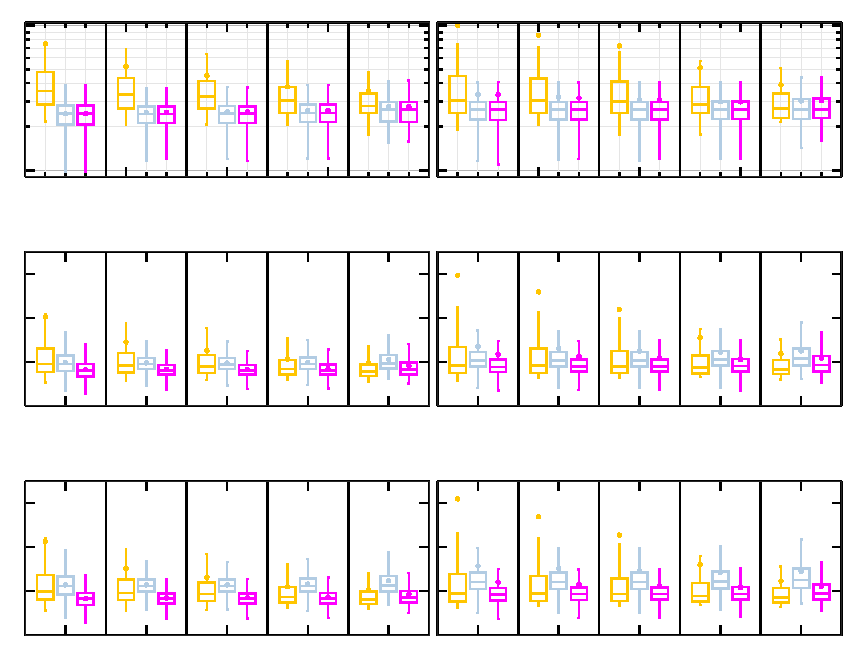
\includegraphics{./figures/parts/02/chapters/04/sections/05/boxplots_iterations}}%
    \gplfronttext
  \end{picture}%
\endgroup

  \end{figure}


  \placebottom
  \tiny [1] C. H. Walsh and S. Karaman, ``CDDT: Fast Approximate 2D Ray Casting for Accelerated Localization,", \textit{IEEE International Conference on Robotics and Automation}, 2018

\note{\footnotesize
Πάμε τώρα στο δεύτερο στόχο. Σε αυτή τη διαφάνεια βλέπουμε τους χρόνους
εκτέλεσης των τριών εκδόσεων του fsm2 για κάθε τιμή θορύβου μέτρησης και
διαφθοράς του χάρτη. Στην άνω σειρά βλέπουμε τα ευθεία αποτελέσματα από την
πειραματική διαδικασία και στην κάτω σειρά τους χρόνους εκτέλεσης που θα είχαν
οι μέθοδοι εάν ο χάρτης αναπαρίστατο ως εικόνα. Η διαφορά ανάμεσα στις δύο
αναπαραστάσεις είναι μεγάλη λόγω του χρόνου υπολογισμού εικονικών σαρώσεων που
είναι η πιό δαπανηρή πράξη, και που στην περίπτωση της αναπαράστασης μέσω
εικόνας μπορεί να γίνει στο ένα τρίτο του χρόνου σε σχέση με τον τρόπου που την
έχω υλοποιήσει εδώ. Τώρα: ο στόχος μας εδώ είναι κάθε μέθοδος να εκτελείται σε
μεγαλύτερη συχνότητα από τη συχνότητα παραγωγής εκτιμήσεων από το σύστημα που
εκτελεί το pose tracking, η οποία δεν έχει ακριβή ορισμό.  Στην πράξη αυτό που
θα θέλαμε είναι η συχνότητα εκτέλεσης να είναι τουλάχιστον 5 Hz.
Ο χαμηλότερος ρυθμός εκτέλεσης είναι της μεθόδου x1 όταν ο χάρτης είναι
διεφθαρμένος, κατά μέσο όρο στα 6.5 Hz, ενώ οι υπόλοιπες δύο μέθοδοι λειτουργούν
με τιμή περίπου στα 13 με 20 Hz.}

\end{frame}

\begin{frame}{\texttt{sm}\{$\cdot$,\texttt{2}\}: \texttt{I/O}}

  \noindent\makebox[\linewidth][c]{%
  \begin{minipage}{\linewidth}
    \begin{minipage}{0.3\linewidth}
      \begin{figure}
        
\definecolor{r}{RGB}{255 69 0}
\definecolor{b}{RGB}{51 102 153}


\tikzset{every picture/.style={line width=0.75pt}} %set default line width to 0.75pt

\begin{tikzpicture}[x=0.75pt,y=0.75pt,yscale=-1,xscale=1]
%uncomment if require: \path (0,300); %set diagram left start at 0, and has height of 300

%Straight Lines [id:da4529423263739871]
\draw   [color={rgb, 255:red, 255; green, 69; blue, 0 }  ] (61.5,52) -- (100.94,83.75) ;
\draw [shift={(102.5,85)}, rotate = 218.83] [color={rgb, 255:red, 255; green, 69; blue, 0 }  ][line width=0.75]    (10.93,-3.29) .. controls (6.95,-1.4) and (3.31,-0.3) .. (0,0) .. controls (3.31,0.3) and (6.95,1.4) .. (10.93,3.29)   ;
%Straight Lines [id:da6488911304441738]
\draw   [color={rgb, 255:red, 51; green, 102; blue, 153 }  ] (58.5,126) -- (100.71,104.89) ;
\draw [shift={(102.5,104)}, rotate = 153.43] [color={rgb, 255:red, 51; green, 102; blue, 153 }  ][line width=0.75]    (10.93,-3.29) .. controls (6.95,-1.4) and (3.31,-0.3) .. (0,0) .. controls (3.31,0.3) and (6.95,1.4) .. (10.93,3.29)   ;
%Straight Lines [id:da5938727374819561]
\draw  [color={rgb, 255:red, 255; green, 69; blue, 0 }  ]  (121.5,37) -- (122.45,75) ;
\draw [shift={(122.5,77)}, rotate = 270] [color={rgb, 255:red, 255; green, 69; blue, 0 }  ][line width=0.75]    (10.93,-3.29) .. controls (6.95,-1.4) and (3.31,-0.3) .. (0,0) .. controls (3.31,0.3) and (6.95,1.4) .. (10.93,3.29)   ;
%Straight Lines [id:da5792126615284177]
\draw    (135.5,94) -- (173.5,94) ;
\draw [shift={(175.5,94)}, rotate = 180] [color={rgb, 255:red, 0; green, 0; blue, 0 }  ][line width=0.75]    (10.93,-3.29) .. controls (6.95,-1.4) and (3.31,-0.3) .. (0,0) .. controls (3.31,0.3) and (6.95,1.4) .. (10.93,3.29)   ;

% Text Node
\draw    (107,82) -- (135,82) -- (135,107) -- (107,107) -- cycle  ;
\draw (121,94.5) node   [align=left] {\texttt{sm}};
% Text Node
\draw (35,32) node [anchor=north west][inner sep=0.75pt]   [align=left] {$\textcolor{r}{\mathcal{S}(\bm{p}_{k})}$};
% Text Node
\draw (34,127) node [anchor=north west][inner sep=0.75pt]   [align=left] {$\textcolor{b}{\mathcal{S}(\bm{p}_{k+1})}$};
% Text Node
\draw (113,17) node [anchor=north west][inner sep=0.75pt]   [align=left] {$\textcolor{r}{\bm{p}_{k}}$};
% Text Node
\draw (179,88) node [anchor=north west][inner sep=0.75pt]   [align=left] {$\textcolor{b}{\bm{p}_{k+1}}$};
\draw  [color={rgb, 255:red, 0; green, 255; blue, 0 }  ]  (195,94) circle [x radius= 16.26, y radius= 16.26]   ;


\end{tikzpicture}
        \caption{\scriptsize \texttt{sm}: ευθυγράμμιση πραγματικών σαρώσεων}
      \end{figure}
    \end{minipage}
    \hspace{1.2cm}
    \begin{minipage}{0.6\linewidth}
      \begin{figure}
        
\definecolor{r}{RGB}{255 69 0}
\definecolor{b}{RGB}{51 102 153}


\tikzset{every picture/.style={line width=0.75pt}} %set default line width to 0.75pt

\begin{tikzpicture}[x=0.75pt,y=0.75pt,yscale=-1,xscale=1]
%uncomment if require: \path (0,300); %set diagram left start at 0, and has height of 300

%Shape: Rectangle [id:dp6131376592433888]
\draw  [dash pattern={on 0.84pt off 2.51pt}] (322,78) -- (519.5,78) -- (519.5,157) -- (322,157) -- cycle ;
%Straight Lines [id:da45736430417167373]
\draw    (294.5,111) -- (325.5,111) ;
\draw [shift={(327.5,111)}, rotate = 180] [color={rgb, 255:red, 0; green, 0; blue, 0 }  ][line width=0.75]    (10.93,-3.29) .. controls (6.95,-1.4) and (3.31,-0.3) .. (0,0) .. controls (3.31,0.3) and (6.95,1.4) .. (10.93,3.29)   ;
%Straight Lines [id:da7019178260598848]
\draw   [color={rgb, 255:red, 51; green, 102; blue, 153 }  ] (293.5,172) -- (470.53,141.34) ;
\draw [shift={(472.5,141)}, rotate = 170.17] [color={rgb, 255:red, 51; green, 102; blue, 153 }  ][line width=0.75]    (10.93,-3.29) .. controls (6.95,-1.4) and (3.31,-0.3) .. (0,0) .. controls (3.31,0.3) and (6.95,1.4) .. (10.93,3.29)   ;
%Straight Lines [id:da9869567554869965]
\draw   [color={rgb, 255:red, 255; green, 69; blue, 0 }  ] (409.5,109) -- (470.56,123.51) ;
\draw [shift={(472.5,124)}, rotate = 194.04] [color={rgb, 255:red, 255; green, 69; blue, 0 }  ][line width=0.75]    (10.93,-3.29) .. controls (6.95,-1.4) and (3.31,-0.3) .. (0,0) .. controls (3.31,0.3) and (6.95,1.4) .. (10.93,3.29)   ;
%Straight Lines [id:da23755426444121874]
\draw    (397.5,37) -- (397.5,89) ;
\draw [shift={(397.5,91)}, rotate = 270] [color={rgb, 255:red, 0; green, 0; blue, 0 }  ][line width=0.75]    (10.93,-3.29) .. controls (6.95,-1.4) and (3.31,-0.3) .. (0,0) .. controls (3.31,0.3) and (6.95,1.4) .. (10.93,3.29)   ;
%Straight Lines [id:da07285087411586999]
\draw   [color={rgb, 255:red, 255; green, 69; blue, 0 }  ] (397.5,37) -- (487.97,112.72) ;
\draw [shift={(489.5,114)}, rotate = 219.93] [color={rgb, 255:red, 255; green, 69; blue, 0 }  ][line width=0.75]    (10.93,-3.29) .. controls (6.95,-1.4) and (3.31,-0.3) .. (0,0) .. controls (3.31,0.3) and (6.95,1.4) .. (10.93,3.29)   ;
%Straight Lines [id:da25729544560038]
\draw    (504.5,132) -- (543.5,132) ;
\draw [shift={(545.5,132)}, rotate = 180] [color={rgb, 255:red, 0; green, 0; blue, 0 }  ][line width=0.75]    (10.93,-3.29) .. controls (6.95,-1.4) and (3.31,-0.3) .. (0,0) .. controls (3.31,0.3) and (6.95,1.4) .. (10.93,3.29)   ;

% Text Node
\draw    (477,119) -- (505,119) -- (505,144) -- (477,144) -- cycle  ;
\draw (491,131.5) node   [align=left] {\texttt{sm}};
% Text Node
\draw (489,58) node [anchor=north west][inner sep=0.75pt]   [align=left] {\texttt{sm2}};
% Text Node
\draw (259,165) node [anchor=north west][inner sep=0.75pt]   [align=left] {$\textcolor{b}{\mathcal{S}(\bm{p})}$};
% Text Node
\draw (224,103) node [anchor=north west][inner sep=0.75pt]   [align=left] {Χάρτης $\bm{M}$};
% Text Node
\draw    (332.1,96) -- (409.1,96) -- (409.1,121) -- (332.1,121) -- cycle  ;
\draw (370.6,111) node   [align=left] {\texttt{scan\_map}};
% Text Node
\draw (393,16) node [anchor=north west][inner sep=0.75pt]   [align=left] {$\textcolor{r}{\hat{\bm{p}}}$};
% Text Node
\draw (422,95) node [anchor=north west][inner sep=0.75pt]   [align=left] {\footnotesize$\textcolor{r}{\mathcal{S}(\hat{\bm{p}})}$};
% Text Node
\draw (549,127) node [anchor=north west][inner sep=0.75pt]   [align=left] {$\textcolor{b}{\bm{p}}$};
\draw  [color={rgb, 255:red, 0; green, 255; blue, 0 }  ]  (556, 133) circle [x radius= 12.26, y radius= 12.26]   ;

\end{tikzpicture}
        \caption{\scriptsize \texttt{sm2}: ευθυγράμμιση πραγματικής σάρωσης με εικονική σάρωση χάρτη}
      \end{figure}
    \end{minipage}

  \end{minipage}
  }


\note{\footnotesize
Σε αυτό το γεγονός κρύβεται μία δεύτερη χρησιμότητα της ευθυγράμμισης σαρώσεων.
Εαν αντικαταστήσουμε τη μία από τις δύο μετρήσεις με μία εικονική σάρωση,
δηλαδή με μία σάρωση που προσομοιώνει την αρχή λειτουργίας του lidar στο χάρτη
αντί για το περιβάλλον, η οποία υπολογίζεται από την εκτίμηση της στάσης του
ρομπότ, τοτε μπορούμε να υπολογίσουμε το μετασχηματισμό ανάμεσα στην εκτίμηση
και την άγνωστη πραγματική στάση του ρομπότ, και αφού γνωρίζουμε την εκτίμηση,
μπορούμε να υπολογίσουμε την πραγματική του στάση.}


\end{frame}



%%%%%%%%%%%%%%%%%%%%%%%%%%%%%%%%%%%%%%%%%%%%%%%%%%%%%%%%%%%%%%%%%%%%%%%%%%%%%%%%
\begin{frame}{Αυτόνομη πλοήγηση: Προαπαιτούμενα}

\definecolor{r}{RGB}{255 0 0}
\definecolor{g}{RGB}{0 255 0}
\definecolor{gr}{RGB}{128 128 128}
\definecolor{b}{RGB}{22 38 252}

\noindent\makebox[\linewidth][c]{%
\begin{minipage}{\linewidth}
  \begin{minipage}{0.4\linewidth}
    \begin{enumerate}
      \item \textcolor{gr}{Εξωδεκτικός αισθητήρας \\ (lidar, rgb(d), sonar)}
      \item \textcolor{gr}{Χάρτης $\bm{M}$ του περιβάλλοντος}
      \item \textcolor{gr}{Εκτίμηση στάσης $\hat{\bm{p}}_t$ \\ (μέσω EKF/PF)}
      \item \textcolor{gr}{Αρχική συνθήκη στάσης $\bm{p}_0^{\bm{M}}$}
      \item \textcolor{gr}{Τελική συνθήκη στάσης $\bm{p}_G^{\bm{M}}$}
    \end{enumerate}
  \end{minipage}
  \hfill
  \begin{minipage}{0.5\linewidth}
    \begin{figure}
      \includegraphics[height=101pt,width=180pt]{./figures/slides/ch3/relief_video_0_imgs/relief_video_0_021}
      \caption{Πηγή: \url{https://relief.web.auth.gr/}}
    \end{figure}
  \end{minipage}
\end{minipage}
}

  \note{\footnotesize Η αυτόνομη πλοήγηση υποθέτει 5 προαπαιτούμενα.}

\end{frame}

\begin{frame}{Τρωτά σημεία μεθόδων ευθυγράμμισης}

  \begin{figure}
    \begin{frame}{Τρωτά σημεία μεθόδων ευθυγράμμισης}

  \begin{figure}
    \input{./figures/slides/ch4/correspondence_is_the_culprit/1.tikz}
  \end{figure}

\note{\footnotesize
Οπότε εδώ γεννάται το φυσικό ερώτημα: ποιά είναι τα τρωτά σημεία των μεθόδων
ευθυγράμμισης σαρώσεων? Με δύο λόγια τα τρωτά σημεία είναι η ευαισθησία της
λύσης στη ρύθμιση των παραμέτρων και στον θόρυβο.}
\end{frame}

  \end{figure}

\note{\footnotesize
Οπότε εδώ γεννάται το φυσικό ερώτημα: ποιά είναι τα τρωτά σημεία των μεθόδων
ευθυγράμμισης σαρώσεων? Με δύο λόγια τα τρωτά σημεία είναι η ευαισθησία της
λύσης στη ρύθμιση των παραμέτρων και στον θόρυβο.}
\end{frame}

\begin{frame}{\small Global localisation: επιλύσιμο μέσω \texttt{sm2}}

  \begin{figure}
    \input{./figures/slides/ch5/sm2_system/sm2_gl_system.tikz}
  \end{figure}

\note{\scriptsize
Το πρόβλημα του global localisation μπορεί να λυθεί μέσω οποιασδήποτε τεχνικής
sm2 ως εξής: δεδομένου του χάρτη του περιβάλλοντος στο οποίο βρίσκεται το
φυσικό ρομπότ, διασπείρονται με τυχαίο τρόπο σε αυτόν ένας αριθμός από
υποθέσεις στάσης, οι οποίες τοποθετούνται σε μία ουρά. Από κάθε υπόθεση
υπολογίζεται η εικονική σάρωση, και στη συνέχεια μέσω sm2 επιχειρείται η
ευθυγράμμιση της με τη σάρωση που συλλαμβάνεται από το φυσικό αισθητήρα. Στο
τέλος κάθε ευθυγράμμισης αποθηκεύονται η τελική εκτίμηση στάσης και η τιμή μίας
μετρικής που αποτυπώνει το βαθμό ομοιότητας ή τελικής ευθυγράμμισης ανάμεσα
στην πραγματική σάρωση και την εικονική σάρωση.  Για τις τεχνικές sm2 που
λειτουργούν με αντιστοιχίσεις αυτό το μέτρο υπολογίζεται εσωτερικά σε κάθε
μέθοδο ως το άθροισμα των αποστάσεων των σημειών της μίας σάρωσης ως προς τα
σημεία, τις γραμμές ή τις κατανομές της δεύτερης, και στο δικό μας σύστημα αυτό
το μέτρο προέρχεται απευθείας από τον FMI-SPOMF. Στο τέλος το σύστημα εξάγει ως
τελική εκτίμηση στάσης εκείνη που σημειώνει τη μεγαλύτερη τιμή ομοιότητας.}

\end{frame}

\begin{frame}{Στόχος Σ2: Χρόνοι εκτέλεσης}

  \vspace{-3.5cm}
  \begin{figure}\centering
    \definecolor{c7}{RGB}{251,180,185}
\definecolor{c8}{RGB}{247,104,161}
\definecolor{c9}{RGB}{255,0,255}

% GNUPLOT: LaTeX picture with Postscript
\begingroup
  \makeatletter
  \providecommand\color[2][]{%
    \GenericError{(gnuplot) \space\space\space\@spaces}{%
      Package color not loaded in conjunction with
      terminal option `colourtext'%
    }{See the gnuplot documentation for explanation.%
    }{Either use 'blacktext' in gnuplot or load the package
      color.sty in LaTeX.}%
    \renewcommand\color[2][]{}%
  }%
  \providecommand\includegraphics[2][]{%
    \GenericError{(gnuplot) \space\space\space\@spaces}{%
      Package graphicx or graphics not loaded%
    }{See the gnuplot documentation for explanation.%
    }{The gnuplot epslatex terminal needs graphicx.sty or graphics.sty.}%
    \renewcommand\includegraphics[2][]{}%
  }%
  \providecommand\rotatebox[2]{#2}%
  \@ifundefined{ifGPcolor}{%
    \newif\ifGPcolor
    \GPcolorfalse
  }{}%
  \@ifundefined{ifGPblacktext}{%
    \newif\ifGPblacktext
    \GPblacktexttrue
  }{}%
  % define a \g@addto@macro without @ in the name:
  \let\gplgaddtomacro\g@addto@macro
  % define empty templates for all commands taking text:
  \gdef\gplfronttext{}%
  \gdef\gplfronttext{}%
  \makeatother
  \ifGPblacktext
    % no textcolor at all
    \def\colorrgb#1{}%
    \def\colorgray#1{}%
  \else
    % gray or color?
    \ifGPcolor
      \def\colorrgb#1{\color[rgb]{#1}}%
      \def\colorgray#1{\color[gray]{#1}}%
      \expandafter\def\csname LTw\endcsname{\color{white}}%
      \expandafter\def\csname LTb\endcsname{\color{black}}%
      \expandafter\def\csname LTa\endcsname{\color{black}}%
      \expandafter\def\csname LT0\endcsname{\color[rgb]{1,0,0}}%
      \expandafter\def\csname LT1\endcsname{\color[rgb]{0,1,0}}%
      \expandafter\def\csname LT2\endcsname{\color[rgb]{0,0,1}}%
      \expandafter\def\csname LT3\endcsname{\color[rgb]{1,0,1}}%
      \expandafter\def\csname LT4\endcsname{\color[rgb]{0,1,1}}%
      \expandafter\def\csname LT5\endcsname{\color[rgb]{1,1,0}}%
      \expandafter\def\csname LT6\endcsname{\color[rgb]{0,0,0}}%
      \expandafter\def\csname LT7\endcsname{\color[rgb]{1,0.3,0}}%
      \expandafter\def\csname LT8\endcsname{\color[rgb]{0.5,0.5,0.5}}%
    \else
      % gray
      \def\colorrgb#1{\color{black}}%
      \def\colorgray#1{\color[gray]{#1}}%
      \expandafter\def\csname LTw\endcsname{\color{white}}%
      \expandafter\def\csname LTb\endcsname{\color{black}}%
      \expandafter\def\csname LTa\endcsname{\color{black}}%
      \expandafter\def\csname LT0\endcsname{\color{black}}%
      \expandafter\def\csname LT1\endcsname{\color{black}}%
      \expandafter\def\csname LT2\endcsname{\color{black}}%
      \expandafter\def\csname LT3\endcsname{\color{black}}%
      \expandafter\def\csname LT4\endcsname{\color{black}}%
      \expandafter\def\csname LT5\endcsname{\color{black}}%
      \expandafter\def\csname LT6\endcsname{\color{black}}%
      \expandafter\def\csname LT7\endcsname{\color{black}}%
      \expandafter\def\csname LT8\endcsname{\color{black}}%
    \fi
  \fi
    \setlength{\unitlength}{0.0500bp}%
    \ifx\gptboxheight\undefined%
      \newlength{\gptboxheight}%
      \newlength{\gptboxwidth}%
      \newsavebox{\gptboxtext}%
    \fi%
    \setlength{\fboxrule}{0.5pt}%
    \setlength{\fboxsep}{1pt}%
\begin{picture}(8000.00,6000.00)%
    \gplgaddtomacro\gplfronttext{%
      \colorrgb{0.15,0.15,0.15}%
      \put(-52,4522){\makebox(0,0)[r]{\strut{}\small $100$}}%
      \colorrgb{0.15,0.15,0.15}%
      \put(-52,4940){\makebox(0,0)[r]{\strut{}\small $200$}}%
      \colorrgb{0.15,0.15,0.15}%
      \put(-52,5184){\makebox(0,0)[r]{\strut{}\small $300$}}%
      \colorrgb{0.15,0.15,0.15}%
      \put(-52,5358){\makebox(0,0)[r]{\strut{}\small $400$}}%
      \colorrgb{0.15,0.15,0.15}%
      \put(-52,5775){\makebox(0,0)[r]{\strut{}\small $800$}}%
      \colorrgb{0.15,0.15,0.15}%
      \put(-52,5910){\makebox(0,0)[r]{\strut{}\small $1000$}}%
      \colorrgb{0.15,0.15,0.15}%
      \put(468,4239){\makebox(0,0){\strut{}}}%
      \colorrgb{0.15,0.15,0.15}%
      \put(1244,4239){\makebox(0,0){\strut{}}}%
      \colorrgb{0.15,0.15,0.15}%
      \put(2020,4239){\makebox(0,0){\strut{}}}%
      \colorrgb{0.15,0.15,0.15}%
      \put(2795,4239){\makebox(0,0){\strut{}}}%
      \colorrgb{0.15,0.15,0.15}%
      \put(3571,4239){\makebox(0,0){\strut{}}}%
    }%
    \gplgaddtomacro\gplfronttext{%
      \colorrgb{0.00,0.00,0.00}%
      \put(3999,6159){\makebox(0,0){\strut{}Κατανομή αριθμού σαρώσεων χάρτη}}%
      \put(2019,6559){\makebox(0,0){\strut{}$\sigma_{\bm{M}} = 0.0$ m}}%
      \put(6019,6559){\makebox(0,0){\strut{}$\sigma_{\bm{M}} = 0.05$ m}}%
      \put(2999,6959){\makebox(0,0){\strut{}{\color{c7}{\rule[0.6mm]{0.5cm}{0.5mm}}}\small x1}}
      \put(3999,6959){\makebox(0,0){\strut{}{\color{c8}{\rule[0.6mm]{0.5cm}{0.5mm}}}\small uf}}
      \put(4999,6959){\makebox(0,0){\strut{}{\color{c9}{\rule[0.6mm]{0.5cm}{0.5mm}}}\small fm}}
    }%
    \gplgaddtomacro\gplfronttext{%
      \colorrgb{0.15,0.15,0.15}%
      \put(3908,4522){\makebox(0,0)[r]{\strut{}}}%
      \colorrgb{0.15,0.15,0.15}%
      \put(3908,4940){\makebox(0,0)[r]{\strut{}}}%
      \colorrgb{0.15,0.15,0.15}%
      \put(3908,5184){\makebox(0,0)[r]{\strut{}}}%
      \colorrgb{0.15,0.15,0.15}%
      \put(3908,5358){\makebox(0,0)[r]{\strut{}}}%
      \colorrgb{0.15,0.15,0.15}%
      \put(3908,5775){\makebox(0,0)[r]{\strut{}}}%
      \colorrgb{0.15,0.15,0.15}%
      \put(3908,5910){\makebox(0,0)[r]{\strut{}}}%
      \colorrgb{0.15,0.15,0.15}%
      \put(4428,4239){\makebox(0,0){\strut{}}}%
      \colorrgb{0.15,0.15,0.15}%
      \put(5204,4239){\makebox(0,0){\strut{}}}%
      \colorrgb{0.15,0.15,0.15}%
      \put(5980,4239){\makebox(0,0){\strut{}}}%
      \colorrgb{0.15,0.15,0.15}%
      \put(6755,4239){\makebox(0,0){\strut{}}}%
      \colorrgb{0.15,0.15,0.15}%
      \put(7531,4239){\makebox(0,0){\strut{}}}%
    }%
    \gplgaddtomacro\gplfronttext{%
    }%
    \gplgaddtomacro\gplfronttext{%
      \colorrgb{0.15,0.15,0.15}%
      \put(-52,2260){\makebox(0,0)[r]{\strut{}\small $0.0$}}%
      \colorrgb{0.15,0.15,0.15}%
      \put(-52,2683){\makebox(0,0)[r]{\strut{}\small $0.100$}}%
      \colorrgb{0.15,0.15,0.15}%
      \put(-52,3105){\makebox(0,0)[r]{\strut{}\small $0.200$}}%
      \colorrgb{0.15,0.15,0.15}%
      \put(-52,3528){\makebox(0,0)[r]{\strut{}\small $0.300$}}%
      \colorrgb{0.15,0.15,0.15}%
      \put(468,2040){\makebox(0,0){\strut{}}}%
      \colorrgb{0.15,0.15,0.15}%
      \put(1244,2040){\makebox(0,0){\strut{}}}%
      \colorrgb{0.15,0.15,0.15}%
      \put(2020,2040){\makebox(0,0){\strut{}}}%
      \colorrgb{0.15,0.15,0.15}%
      \put(2795,2040){\makebox(0,0){\strut{}}}%
      \colorrgb{0.15,0.15,0.15}%
      \put(3571,2040){\makebox(0,0){\strut{}}}%
    }%
    \gplgaddtomacro\gplfronttext{%
      \colorrgb{0.00,0.00,0.00}%
      \put(3999,3959){\makebox(0,0){\strut{}Κατανομή ολικού χρόνου εκτέλεσης [sec]}}%
    }%
    \gplgaddtomacro\gplfronttext{%
      \colorrgb{0.15,0.15,0.15}%
      \put(3908,2260){\makebox(0,0)[r]{\strut{}}}%
      \colorrgb{0.15,0.15,0.15}%
      \put(3908,2683){\makebox(0,0)[r]{\strut{}}}%
      \colorrgb{0.15,0.15,0.15}%
      \put(3908,3105){\makebox(0,0)[r]{\strut{}}}%
      \colorrgb{0.15,0.15,0.15}%
      \put(3908,3528){\makebox(0,0)[r]{\strut{}}}%
      \colorrgb{0.15,0.15,0.15}%
      \put(4428,2040){\makebox(0,0){\strut{}}}%
      \colorrgb{0.15,0.15,0.15}%
      \put(5204,2040){\makebox(0,0){\strut{}}}%
      \colorrgb{0.15,0.15,0.15}%
      \put(5980,2040){\makebox(0,0){\strut{}}}%
      \colorrgb{0.15,0.15,0.15}%
      \put(6755,2040){\makebox(0,0){\strut{}}}%
      \colorrgb{0.15,0.15,0.15}%
      \put(7531,2040){\makebox(0,0){\strut{}}}%
    }%
    \gplgaddtomacro\gplfronttext{%
    }%
    \gplgaddtomacro\gplfronttext{%
      \colorrgb{0.15,0.15,0.15}%
      \put(-52,60){\makebox(0,0)[r]{\strut{}\small $0.0$}}%
      \colorrgb{0.15,0.15,0.15}%
      \put(-52,483){\makebox(0,0)[r]{\strut{}\small $0.050$}}%
      \colorrgb{0.15,0.15,0.15}%
      \put(-52,905){\makebox(0,0)[r]{\strut{}\small $0.100$}}%
      \colorrgb{0.15,0.15,0.15}%
      \put(-52,1328){\makebox(0,0)[r]{\strut{}\small $0.150$}}%
      \colorrgb{0.15,0.15,0.15}%
      \put(468,-160){\makebox(0,0){\strut{}$0.01$}}%
      \colorrgb{0.15,0.15,0.15}%
      \put(1244,-160){\makebox(0,0){\strut{}$0.03$}}%
      \colorrgb{0.15,0.15,0.15}%
      \put(2020,-160){\makebox(0,0){\strut{}$0.05$}}%
      \colorrgb{0.15,0.15,0.15}%
      \put(2795,-160){\makebox(0,0){\strut{}$0.10$}}%
      \colorrgb{0.15,0.15,0.15}%
      \put(3571,-160){\makebox(0,0){\strut{}$0.20$}}%
    }%
    \gplgaddtomacro\gplfronttext{%
      \colorrgb{0.15,0.15,0.15}%
      \put(3999,-490){\makebox(0,0){\strut{}Τυπική απόκλιση διαταραχών $\sigma_R$ [m]}}%
      \colorrgb{0.00,0.00,0.00}%
      \put(3999,1759){\makebox(0,0){\strut{}Κατανομή ολικού χρόνου εκτέλεσης [sec] (Αναγωγή σε αναπαράσταση χάρτη μέσω πλέγματος)}}%
    }%
    \gplgaddtomacro\gplfronttext{%
      \colorrgb{0.15,0.15,0.15}%
      \put(3908,60){\makebox(0,0)[r]{\strut{}}}%
      \colorrgb{0.15,0.15,0.15}%
      \put(3908,483){\makebox(0,0)[r]{\strut{}}}%
      \colorrgb{0.15,0.15,0.15}%
      \put(3908,905){\makebox(0,0)[r]{\strut{}}}%
      \colorrgb{0.15,0.15,0.15}%
      \put(3908,1328){\makebox(0,0)[r]{\strut{}}}%
      \colorrgb{0.15,0.15,0.15}%
      \put(4428,-160){\makebox(0,0){\strut{}$0.01$}}%
      \colorrgb{0.15,0.15,0.15}%
      \put(5204,-160){\makebox(0,0){\strut{}$0.03$}}%
      \colorrgb{0.15,0.15,0.15}%
      \put(5980,-160){\makebox(0,0){\strut{}$0.05$}}%
      \colorrgb{0.15,0.15,0.15}%
      \put(6755,-160){\makebox(0,0){\strut{}$0.10$}}%
      \colorrgb{0.15,0.15,0.15}%
      \put(7531,-160){\makebox(0,0){\strut{}$0.20$}}%
    }%
    \gplgaddtomacro\gplfronttext{%
    }%
    \put(0,0){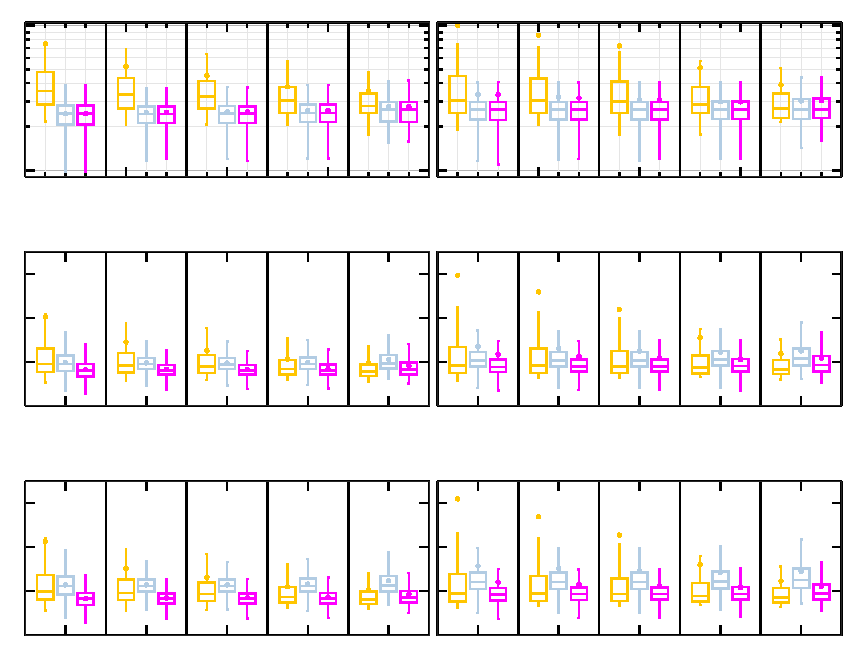
\includegraphics{./figures/parts/02/chapters/04/sections/05/boxplots_iterations}}%
    \gplfronttext
  \end{picture}%
\endgroup

  \end{figure}


  \placebottom
  \tiny [1] C. H. Walsh and S. Karaman, ``CDDT: Fast Approximate 2D Ray Casting for Accelerated Localization,", \textit{IEEE International Conference on Robotics and Automation}, 2018

\note{\footnotesize
Πάμε τώρα στο δεύτερο στόχο. Σε αυτή τη διαφάνεια βλέπουμε τους χρόνους
εκτέλεσης των τριών εκδόσεων του fsm2 για κάθε τιμή θορύβου μέτρησης και
διαφθοράς του χάρτη. Στην άνω σειρά βλέπουμε τα ευθεία αποτελέσματα από την
πειραματική διαδικασία και στην κάτω σειρά τους χρόνους εκτέλεσης που θα είχαν
οι μέθοδοι εάν ο χάρτης αναπαρίστατο ως εικόνα. Η διαφορά ανάμεσα στις δύο
αναπαραστάσεις είναι μεγάλη λόγω του χρόνου υπολογισμού εικονικών σαρώσεων που
είναι η πιό δαπανηρή πράξη, και που στην περίπτωση της αναπαράστασης μέσω
εικόνας μπορεί να γίνει στο ένα τρίτο του χρόνου σε σχέση με τον τρόπου που την
έχω υλοποιήσει εδώ. Τώρα: ο στόχος μας εδώ είναι κάθε μέθοδος να εκτελείται σε
μεγαλύτερη συχνότητα από τη συχνότητα παραγωγής εκτιμήσεων από το σύστημα που
εκτελεί το pose tracking, η οποία δεν έχει ακριβή ορισμό.  Στην πράξη αυτό που
θα θέλαμε είναι η συχνότητα εκτέλεσης να είναι τουλάχιστον 5 Hz.
Ο χαμηλότερος ρυθμός εκτέλεσης είναι της μεθόδου x1 όταν ο χάρτης είναι
διεφθαρμένος, κατά μέσο όρο στα 6.5 Hz, ενώ οι υπόλοιπες δύο μέθοδοι λειτουργούν
με τιμή περίπου στα 13 με 20 Hz.}

\end{frame}

\begin{frame}{\texttt{sm}\{$\cdot$,\texttt{2}\}: \texttt{I/O}}

  \noindent\makebox[\linewidth][c]{%
  \begin{minipage}{\linewidth}
    \begin{minipage}{0.3\linewidth}
      \begin{figure}
        
\definecolor{r}{RGB}{255 69 0}
\definecolor{b}{RGB}{51 102 153}


\tikzset{every picture/.style={line width=0.75pt}} %set default line width to 0.75pt

\begin{tikzpicture}[x=0.75pt,y=0.75pt,yscale=-1,xscale=1]
%uncomment if require: \path (0,300); %set diagram left start at 0, and has height of 300

%Straight Lines [id:da4529423263739871]
\draw   [color={rgb, 255:red, 255; green, 69; blue, 0 }  ] (61.5,52) -- (100.94,83.75) ;
\draw [shift={(102.5,85)}, rotate = 218.83] [color={rgb, 255:red, 255; green, 69; blue, 0 }  ][line width=0.75]    (10.93,-3.29) .. controls (6.95,-1.4) and (3.31,-0.3) .. (0,0) .. controls (3.31,0.3) and (6.95,1.4) .. (10.93,3.29)   ;
%Straight Lines [id:da6488911304441738]
\draw   [color={rgb, 255:red, 51; green, 102; blue, 153 }  ] (58.5,126) -- (100.71,104.89) ;
\draw [shift={(102.5,104)}, rotate = 153.43] [color={rgb, 255:red, 51; green, 102; blue, 153 }  ][line width=0.75]    (10.93,-3.29) .. controls (6.95,-1.4) and (3.31,-0.3) .. (0,0) .. controls (3.31,0.3) and (6.95,1.4) .. (10.93,3.29)   ;
%Straight Lines [id:da5938727374819561]
\draw  [color={rgb, 255:red, 255; green, 69; blue, 0 }  ]  (121.5,37) -- (122.45,75) ;
\draw [shift={(122.5,77)}, rotate = 270] [color={rgb, 255:red, 255; green, 69; blue, 0 }  ][line width=0.75]    (10.93,-3.29) .. controls (6.95,-1.4) and (3.31,-0.3) .. (0,0) .. controls (3.31,0.3) and (6.95,1.4) .. (10.93,3.29)   ;
%Straight Lines [id:da5792126615284177]
\draw    (135.5,94) -- (173.5,94) ;
\draw [shift={(175.5,94)}, rotate = 180] [color={rgb, 255:red, 0; green, 0; blue, 0 }  ][line width=0.75]    (10.93,-3.29) .. controls (6.95,-1.4) and (3.31,-0.3) .. (0,0) .. controls (3.31,0.3) and (6.95,1.4) .. (10.93,3.29)   ;

% Text Node
\draw    (107,82) -- (135,82) -- (135,107) -- (107,107) -- cycle  ;
\draw (121,94.5) node   [align=left] {\texttt{sm}};
% Text Node
\draw (35,32) node [anchor=north west][inner sep=0.75pt]   [align=left] {$\textcolor{r}{\mathcal{S}(\bm{p}_{k})}$};
% Text Node
\draw (34,127) node [anchor=north west][inner sep=0.75pt]   [align=left] {$\textcolor{b}{\mathcal{S}(\bm{p}_{k+1})}$};
% Text Node
\draw (113,17) node [anchor=north west][inner sep=0.75pt]   [align=left] {$\textcolor{r}{\bm{p}_{k}}$};
% Text Node
\draw (179,88) node [anchor=north west][inner sep=0.75pt]   [align=left] {$\textcolor{b}{\bm{p}_{k+1}}$};
\draw  [color={rgb, 255:red, 0; green, 255; blue, 0 }  ]  (195,94) circle [x radius= 16.26, y radius= 16.26]   ;


\end{tikzpicture}
        \caption{\scriptsize \texttt{sm}: ευθυγράμμιση πραγματικών σαρώσεων}
      \end{figure}
    \end{minipage}
    \hspace{1.2cm}
    \begin{minipage}{0.6\linewidth}
      \begin{figure}
        
\definecolor{r}{RGB}{255 69 0}
\definecolor{b}{RGB}{51 102 153}


\tikzset{every picture/.style={line width=0.75pt}} %set default line width to 0.75pt

\begin{tikzpicture}[x=0.75pt,y=0.75pt,yscale=-1,xscale=1]
%uncomment if require: \path (0,300); %set diagram left start at 0, and has height of 300

%Shape: Rectangle [id:dp6131376592433888]
\draw  [dash pattern={on 0.84pt off 2.51pt}] (322,78) -- (519.5,78) -- (519.5,157) -- (322,157) -- cycle ;
%Straight Lines [id:da45736430417167373]
\draw    (294.5,111) -- (325.5,111) ;
\draw [shift={(327.5,111)}, rotate = 180] [color={rgb, 255:red, 0; green, 0; blue, 0 }  ][line width=0.75]    (10.93,-3.29) .. controls (6.95,-1.4) and (3.31,-0.3) .. (0,0) .. controls (3.31,0.3) and (6.95,1.4) .. (10.93,3.29)   ;
%Straight Lines [id:da7019178260598848]
\draw   [color={rgb, 255:red, 51; green, 102; blue, 153 }  ] (293.5,172) -- (470.53,141.34) ;
\draw [shift={(472.5,141)}, rotate = 170.17] [color={rgb, 255:red, 51; green, 102; blue, 153 }  ][line width=0.75]    (10.93,-3.29) .. controls (6.95,-1.4) and (3.31,-0.3) .. (0,0) .. controls (3.31,0.3) and (6.95,1.4) .. (10.93,3.29)   ;
%Straight Lines [id:da9869567554869965]
\draw   [color={rgb, 255:red, 255; green, 69; blue, 0 }  ] (409.5,109) -- (470.56,123.51) ;
\draw [shift={(472.5,124)}, rotate = 194.04] [color={rgb, 255:red, 255; green, 69; blue, 0 }  ][line width=0.75]    (10.93,-3.29) .. controls (6.95,-1.4) and (3.31,-0.3) .. (0,0) .. controls (3.31,0.3) and (6.95,1.4) .. (10.93,3.29)   ;
%Straight Lines [id:da23755426444121874]
\draw    (397.5,37) -- (397.5,89) ;
\draw [shift={(397.5,91)}, rotate = 270] [color={rgb, 255:red, 0; green, 0; blue, 0 }  ][line width=0.75]    (10.93,-3.29) .. controls (6.95,-1.4) and (3.31,-0.3) .. (0,0) .. controls (3.31,0.3) and (6.95,1.4) .. (10.93,3.29)   ;
%Straight Lines [id:da07285087411586999]
\draw   [color={rgb, 255:red, 255; green, 69; blue, 0 }  ] (397.5,37) -- (487.97,112.72) ;
\draw [shift={(489.5,114)}, rotate = 219.93] [color={rgb, 255:red, 255; green, 69; blue, 0 }  ][line width=0.75]    (10.93,-3.29) .. controls (6.95,-1.4) and (3.31,-0.3) .. (0,0) .. controls (3.31,0.3) and (6.95,1.4) .. (10.93,3.29)   ;
%Straight Lines [id:da25729544560038]
\draw    (504.5,132) -- (543.5,132) ;
\draw [shift={(545.5,132)}, rotate = 180] [color={rgb, 255:red, 0; green, 0; blue, 0 }  ][line width=0.75]    (10.93,-3.29) .. controls (6.95,-1.4) and (3.31,-0.3) .. (0,0) .. controls (3.31,0.3) and (6.95,1.4) .. (10.93,3.29)   ;

% Text Node
\draw    (477,119) -- (505,119) -- (505,144) -- (477,144) -- cycle  ;
\draw (491,131.5) node   [align=left] {\texttt{sm}};
% Text Node
\draw (489,58) node [anchor=north west][inner sep=0.75pt]   [align=left] {\texttt{sm2}};
% Text Node
\draw (259,165) node [anchor=north west][inner sep=0.75pt]   [align=left] {$\textcolor{b}{\mathcal{S}(\bm{p})}$};
% Text Node
\draw (224,103) node [anchor=north west][inner sep=0.75pt]   [align=left] {Χάρτης $\bm{M}$};
% Text Node
\draw    (332.1,96) -- (409.1,96) -- (409.1,121) -- (332.1,121) -- cycle  ;
\draw (370.6,111) node   [align=left] {\texttt{scan\_map}};
% Text Node
\draw (393,16) node [anchor=north west][inner sep=0.75pt]   [align=left] {$\textcolor{r}{\hat{\bm{p}}}$};
% Text Node
\draw (422,95) node [anchor=north west][inner sep=0.75pt]   [align=left] {\footnotesize$\textcolor{r}{\mathcal{S}(\hat{\bm{p}})}$};
% Text Node
\draw (549,127) node [anchor=north west][inner sep=0.75pt]   [align=left] {$\textcolor{b}{\bm{p}}$};
\draw  [color={rgb, 255:red, 0; green, 255; blue, 0 }  ]  (556, 133) circle [x radius= 12.26, y radius= 12.26]   ;

\end{tikzpicture}
        \caption{\scriptsize \texttt{sm2}: ευθυγράμμιση πραγματικής σάρωσης με εικονική σάρωση χάρτη}
      \end{figure}
    \end{minipage}

  \end{minipage}
  }


\note{\footnotesize
Σε αυτό το γεγονός κρύβεται μία δεύτερη χρησιμότητα της ευθυγράμμισης σαρώσεων.
Εαν αντικαταστήσουμε τη μία από τις δύο μετρήσεις με μία εικονική σάρωση,
δηλαδή με μία σάρωση που προσομοιώνει την αρχή λειτουργίας του lidar στο χάρτη
αντί για το περιβάλλον, η οποία υπολογίζεται από την εκτίμηση της στάσης του
ρομπότ, τοτε μπορούμε να υπολογίσουμε το μετασχηματισμό ανάμεσα στην εκτίμηση
και την άγνωστη πραγματική στάση του ρομπότ, και αφού γνωρίζουμε την εκτίμηση,
μπορούμε να υπολογίσουμε την πραγματική του στάση.}


\end{frame}



%%%%%%%%%%%%%%%%%%%%%%%%%%%%%%%%%%%%%%%%%%%%%%%%%%%%%%%%%%%%%%%%%%%%%%%%%%%%%%%%
%\begin{frame}{Αυτόνομη πλοήγηση: Προαπαιτούμενα}

\definecolor{r}{RGB}{255 0 0}
\definecolor{g}{RGB}{0 255 0}
\definecolor{gr}{RGB}{128 128 128}
\definecolor{b}{RGB}{22 38 252}

\noindent\makebox[\linewidth][c]{%
\begin{minipage}{\linewidth}
  \begin{minipage}{0.4\linewidth}
    \begin{enumerate}
      \item \textcolor{gr}{Εξωδεκτικός αισθητήρας \\ (lidar, rgb(d), sonar)}
      \item \textcolor{gr}{Χάρτης $\bm{M}$ του περιβάλλοντος}
      \item \textcolor{gr}{Εκτίμηση στάσης $\hat{\bm{p}}_t$ \\ (μέσω EKF/PF)}
      \item \textcolor{gr}{Αρχική συνθήκη στάσης $\bm{p}_0^{\bm{M}}$}
      \item \textcolor{gr}{Τελική συνθήκη στάσης $\bm{p}_G^{\bm{M}}$}
    \end{enumerate}
  \end{minipage}
  \hfill
  \begin{minipage}{0.5\linewidth}
    \begin{figure}
      \includegraphics[height=101pt,width=180pt]{./figures/slides/ch3/relief_video_0_imgs/relief_video_0_021}
      \caption{Πηγή: \url{https://relief.web.auth.gr/}}
    \end{figure}
  \end{minipage}
\end{minipage}
}

  \note{\footnotesize Η αυτόνομη πλοήγηση υποθέτει 5 προαπαιτούμενα.}

\end{frame}

\begin{frame}{Τρωτά σημεία μεθόδων ευθυγράμμισης}

  \begin{figure}
    \input{./figures/slides/ch4/correspondence_is_the_culprit/1.tikz}
  \end{figure}

\note{\footnotesize
Οπότε εδώ γεννάται το φυσικό ερώτημα: ποιά είναι τα τρωτά σημεία των μεθόδων
ευθυγράμμισης σαρώσεων? Με δύο λόγια τα τρωτά σημεία είναι η ευαισθησία της
λύσης στη ρύθμιση των παραμέτρων και στον θόρυβο.}
\end{frame}

\begin{frame}{\small Global localisation: επιλύσιμο μέσω \texttt{sm2}}

  \begin{figure}
    \input{./figures/slides/ch5/sm2_system/sm2_gl_system.tikz}
  \end{figure}

\note{\scriptsize
Το πρόβλημα του global localisation μπορεί να λυθεί μέσω οποιασδήποτε τεχνικής
sm2 ως εξής: δεδομένου του χάρτη του περιβάλλοντος στο οποίο βρίσκεται το
φυσικό ρομπότ, διασπείρονται με τυχαίο τρόπο σε αυτόν ένας αριθμός από
υποθέσεις στάσης, οι οποίες τοποθετούνται σε μία ουρά. Από κάθε υπόθεση
υπολογίζεται η εικονική σάρωση, και στη συνέχεια μέσω sm2 επιχειρείται η
ευθυγράμμιση της με τη σάρωση που συλλαμβάνεται από το φυσικό αισθητήρα. Στο
τέλος κάθε ευθυγράμμισης αποθηκεύονται η τελική εκτίμηση στάσης και η τιμή μίας
μετρικής που αποτυπώνει το βαθμό ομοιότητας ή τελικής ευθυγράμμισης ανάμεσα
στην πραγματική σάρωση και την εικονική σάρωση.  Για τις τεχνικές sm2 που
λειτουργούν με αντιστοιχίσεις αυτό το μέτρο υπολογίζεται εσωτερικά σε κάθε
μέθοδο ως το άθροισμα των αποστάσεων των σημειών της μίας σάρωσης ως προς τα
σημεία, τις γραμμές ή τις κατανομές της δεύτερης, και στο δικό μας σύστημα αυτό
το μέτρο προέρχεται απευθείας από τον FMI-SPOMF. Στο τέλος το σύστημα εξάγει ως
τελική εκτίμηση στάσης εκείνη που σημειώνει τη μεγαλύτερη τιμή ομοιότητας.}

\end{frame}

\begin{frame}{Στόχος Σ2: Χρόνοι εκτέλεσης}

  \vspace{-3.5cm}
  \begin{figure}\centering
    \input{./figures/slides/ch6/experiments/boxplots_iterations.tex}
  \end{figure}


  \placebottom
  \tiny [1] C. H. Walsh and S. Karaman, ``CDDT: Fast Approximate 2D Ray Casting for Accelerated Localization,", \textit{IEEE International Conference on Robotics and Automation}, 2018

\note{\footnotesize
Πάμε τώρα στο δεύτερο στόχο. Σε αυτή τη διαφάνεια βλέπουμε τους χρόνους
εκτέλεσης των τριών εκδόσεων του fsm2 για κάθε τιμή θορύβου μέτρησης και
διαφθοράς του χάρτη. Στην άνω σειρά βλέπουμε τα ευθεία αποτελέσματα από την
πειραματική διαδικασία και στην κάτω σειρά τους χρόνους εκτέλεσης που θα είχαν
οι μέθοδοι εάν ο χάρτης αναπαρίστατο ως εικόνα. Η διαφορά ανάμεσα στις δύο
αναπαραστάσεις είναι μεγάλη λόγω του χρόνου υπολογισμού εικονικών σαρώσεων που
είναι η πιό δαπανηρή πράξη, και που στην περίπτωση της αναπαράστασης μέσω
εικόνας μπορεί να γίνει στο ένα τρίτο του χρόνου σε σχέση με τον τρόπου που την
έχω υλοποιήσει εδώ. Τώρα: ο στόχος μας εδώ είναι κάθε μέθοδος να εκτελείται σε
μεγαλύτερη συχνότητα από τη συχνότητα παραγωγής εκτιμήσεων από το σύστημα που
εκτελεί το pose tracking, η οποία δεν έχει ακριβή ορισμό.  Στην πράξη αυτό που
θα θέλαμε είναι η συχνότητα εκτέλεσης να είναι τουλάχιστον 5 Hz.
Ο χαμηλότερος ρυθμός εκτέλεσης είναι της μεθόδου x1 όταν ο χάρτης είναι
διεφθαρμένος, κατά μέσο όρο στα 6.5 Hz, ενώ οι υπόλοιπες δύο μέθοδοι λειτουργούν
με τιμή περίπου στα 13 με 20 Hz.}

\end{frame}

\begin{frame}{\texttt{sm}\{$\cdot$,\texttt{2}\}: \texttt{I/O}}

  \noindent\makebox[\linewidth][c]{%
  \begin{minipage}{\linewidth}
    \begin{minipage}{0.3\linewidth}
      \begin{figure}
        \input{./figures/slides/ch4/sm_smsm_1.tikz}
        \caption{\scriptsize \texttt{sm}: ευθυγράμμιση πραγματικών σαρώσεων}
      \end{figure}
    \end{minipage}
    \hspace{1.2cm}
    \begin{minipage}{0.6\linewidth}
      \begin{figure}
        \input{./figures/slides/ch4/sm_smsm_2.tikz}
        \caption{\scriptsize \texttt{sm2}: ευθυγράμμιση πραγματικής σάρωσης με εικονική σάρωση χάρτη}
      \end{figure}
    \end{minipage}

  \end{minipage}
  }


\note{\footnotesize
Σε αυτό το γεγονός κρύβεται μία δεύτερη χρησιμότητα της ευθυγράμμισης σαρώσεων.
Εαν αντικαταστήσουμε τη μία από τις δύο μετρήσεις με μία εικονική σάρωση,
δηλαδή με μία σάρωση που προσομοιώνει την αρχή λειτουργίας του lidar στο χάρτη
αντί για το περιβάλλον, η οποία υπολογίζεται από την εκτίμηση της στάσης του
ρομπότ, τοτε μπορούμε να υπολογίσουμε το μετασχηματισμό ανάμεσα στην εκτίμηση
και την άγνωστη πραγματική στάση του ρομπότ, και αφού γνωρίζουμε την εκτίμηση,
μπορούμε να υπολογίσουμε την πραγματική του στάση.}


\end{frame}


%\begin{frame}{Αυτόνομη πλοήγηση: Προαπαιτούμενα}

\definecolor{r}{RGB}{255 0 0}
\definecolor{g}{RGB}{0 255 0}
\definecolor{gr}{RGB}{128 128 128}
\definecolor{b}{RGB}{22 38 252}

\noindent\makebox[\linewidth][c]{%
\begin{minipage}{\linewidth}
  \begin{minipage}{0.4\linewidth}
    \begin{enumerate}
      \item \textcolor{gr}{Εξωδεκτικός αισθητήρας \\ (lidar, rgb(d), sonar)}
      \item \textcolor{gr}{Χάρτης $\bm{M}$ του περιβάλλοντος}
      \item \textcolor{gr}{Εκτίμηση στάσης $\hat{\bm{p}}_t$ \\ (μέσω EKF/PF)}
      \item \textcolor{gr}{Αρχική συνθήκη στάσης $\bm{p}_0^{\bm{M}}$}
      \item \textcolor{gr}{Τελική συνθήκη στάσης $\bm{p}_G^{\bm{M}}$}
    \end{enumerate}
  \end{minipage}
  \hfill
  \begin{minipage}{0.5\linewidth}
    \begin{figure}
      \includegraphics[height=101pt,width=180pt]{./figures/slides/ch3/relief_video_0_imgs/relief_video_0_021}
      \caption{Πηγή: \url{https://relief.web.auth.gr/}}
    \end{figure}
  \end{minipage}
\end{minipage}
}

  \note{\footnotesize Η αυτόνομη πλοήγηση υποθέτει 5 προαπαιτούμενα.}

\end{frame}

\begin{frame}{Τρωτά σημεία μεθόδων ευθυγράμμισης}

  \begin{figure}
    \input{./figures/slides/ch4/correspondence_is_the_culprit/1.tikz}
  \end{figure}

\note{\footnotesize
Οπότε εδώ γεννάται το φυσικό ερώτημα: ποιά είναι τα τρωτά σημεία των μεθόδων
ευθυγράμμισης σαρώσεων? Με δύο λόγια τα τρωτά σημεία είναι η ευαισθησία της
λύσης στη ρύθμιση των παραμέτρων και στον θόρυβο.}
\end{frame}

\begin{frame}{\small Global localisation: επιλύσιμο μέσω \texttt{sm2}}

  \begin{figure}
    \input{./figures/slides/ch5/sm2_system/sm2_gl_system.tikz}
  \end{figure}

\note{\scriptsize
Το πρόβλημα του global localisation μπορεί να λυθεί μέσω οποιασδήποτε τεχνικής
sm2 ως εξής: δεδομένου του χάρτη του περιβάλλοντος στο οποίο βρίσκεται το
φυσικό ρομπότ, διασπείρονται με τυχαίο τρόπο σε αυτόν ένας αριθμός από
υποθέσεις στάσης, οι οποίες τοποθετούνται σε μία ουρά. Από κάθε υπόθεση
υπολογίζεται η εικονική σάρωση, και στη συνέχεια μέσω sm2 επιχειρείται η
ευθυγράμμιση της με τη σάρωση που συλλαμβάνεται από το φυσικό αισθητήρα. Στο
τέλος κάθε ευθυγράμμισης αποθηκεύονται η τελική εκτίμηση στάσης και η τιμή μίας
μετρικής που αποτυπώνει το βαθμό ομοιότητας ή τελικής ευθυγράμμισης ανάμεσα
στην πραγματική σάρωση και την εικονική σάρωση.  Για τις τεχνικές sm2 που
λειτουργούν με αντιστοιχίσεις αυτό το μέτρο υπολογίζεται εσωτερικά σε κάθε
μέθοδο ως το άθροισμα των αποστάσεων των σημειών της μίας σάρωσης ως προς τα
σημεία, τις γραμμές ή τις κατανομές της δεύτερης, και στο δικό μας σύστημα αυτό
το μέτρο προέρχεται απευθείας από τον FMI-SPOMF. Στο τέλος το σύστημα εξάγει ως
τελική εκτίμηση στάσης εκείνη που σημειώνει τη μεγαλύτερη τιμή ομοιότητας.}

\end{frame}

\begin{frame}{Στόχος Σ2: Χρόνοι εκτέλεσης}

  \vspace{-3.5cm}
  \begin{figure}\centering
    \input{./figures/slides/ch6/experiments/boxplots_iterations.tex}
  \end{figure}


  \placebottom
  \tiny [1] C. H. Walsh and S. Karaman, ``CDDT: Fast Approximate 2D Ray Casting for Accelerated Localization,", \textit{IEEE International Conference on Robotics and Automation}, 2018

\note{\footnotesize
Πάμε τώρα στο δεύτερο στόχο. Σε αυτή τη διαφάνεια βλέπουμε τους χρόνους
εκτέλεσης των τριών εκδόσεων του fsm2 για κάθε τιμή θορύβου μέτρησης και
διαφθοράς του χάρτη. Στην άνω σειρά βλέπουμε τα ευθεία αποτελέσματα από την
πειραματική διαδικασία και στην κάτω σειρά τους χρόνους εκτέλεσης που θα είχαν
οι μέθοδοι εάν ο χάρτης αναπαρίστατο ως εικόνα. Η διαφορά ανάμεσα στις δύο
αναπαραστάσεις είναι μεγάλη λόγω του χρόνου υπολογισμού εικονικών σαρώσεων που
είναι η πιό δαπανηρή πράξη, και που στην περίπτωση της αναπαράστασης μέσω
εικόνας μπορεί να γίνει στο ένα τρίτο του χρόνου σε σχέση με τον τρόπου που την
έχω υλοποιήσει εδώ. Τώρα: ο στόχος μας εδώ είναι κάθε μέθοδος να εκτελείται σε
μεγαλύτερη συχνότητα από τη συχνότητα παραγωγής εκτιμήσεων από το σύστημα που
εκτελεί το pose tracking, η οποία δεν έχει ακριβή ορισμό.  Στην πράξη αυτό που
θα θέλαμε είναι η συχνότητα εκτέλεσης να είναι τουλάχιστον 5 Hz.
Ο χαμηλότερος ρυθμός εκτέλεσης είναι της μεθόδου x1 όταν ο χάρτης είναι
διεφθαρμένος, κατά μέσο όρο στα 6.5 Hz, ενώ οι υπόλοιπες δύο μέθοδοι λειτουργούν
με τιμή περίπου στα 13 με 20 Hz.}

\end{frame}

\begin{frame}{\texttt{sm}\{$\cdot$,\texttt{2}\}: \texttt{I/O}}

  \noindent\makebox[\linewidth][c]{%
  \begin{minipage}{\linewidth}
    \begin{minipage}{0.3\linewidth}
      \begin{figure}
        \input{./figures/slides/ch4/sm_smsm_1.tikz}
        \caption{\scriptsize \texttt{sm}: ευθυγράμμιση πραγματικών σαρώσεων}
      \end{figure}
    \end{minipage}
    \hspace{1.2cm}
    \begin{minipage}{0.6\linewidth}
      \begin{figure}
        \input{./figures/slides/ch4/sm_smsm_2.tikz}
        \caption{\scriptsize \texttt{sm2}: ευθυγράμμιση πραγματικής σάρωσης με εικονική σάρωση χάρτη}
      \end{figure}
    \end{minipage}

  \end{minipage}
  }


\note{\footnotesize
Σε αυτό το γεγονός κρύβεται μία δεύτερη χρησιμότητα της ευθυγράμμισης σαρώσεων.
Εαν αντικαταστήσουμε τη μία από τις δύο μετρήσεις με μία εικονική σάρωση,
δηλαδή με μία σάρωση που προσομοιώνει την αρχή λειτουργίας του lidar στο χάρτη
αντί για το περιβάλλον, η οποία υπολογίζεται από την εκτίμηση της στάσης του
ρομπότ, τοτε μπορούμε να υπολογίσουμε το μετασχηματισμό ανάμεσα στην εκτίμηση
και την άγνωστη πραγματική στάση του ρομπότ, και αφού γνωρίζουμε την εκτίμηση,
μπορούμε να υπολογίσουμε την πραγματική του στάση.}


\end{frame}


%\begin{frame}{Αυτόνομη πλοήγηση: Προαπαιτούμενα}

\definecolor{r}{RGB}{255 0 0}
\definecolor{g}{RGB}{0 255 0}
\definecolor{gr}{RGB}{128 128 128}
\definecolor{b}{RGB}{22 38 252}

\noindent\makebox[\linewidth][c]{%
\begin{minipage}{\linewidth}
  \begin{minipage}{0.4\linewidth}
    \begin{enumerate}
      \item \textcolor{gr}{Εξωδεκτικός αισθητήρας \\ (lidar, rgb(d), sonar)}
      \item \textcolor{gr}{Χάρτης $\bm{M}$ του περιβάλλοντος}
      \item \textcolor{gr}{Εκτίμηση στάσης $\hat{\bm{p}}_t$ \\ (μέσω EKF/PF)}
      \item \textcolor{gr}{Αρχική συνθήκη στάσης $\bm{p}_0^{\bm{M}}$}
      \item \textcolor{gr}{Τελική συνθήκη στάσης $\bm{p}_G^{\bm{M}}$}
    \end{enumerate}
  \end{minipage}
  \hfill
  \begin{minipage}{0.5\linewidth}
    \begin{figure}
      \includegraphics[height=101pt,width=180pt]{./figures/slides/ch3/relief_video_0_imgs/relief_video_0_021}
      \caption{Πηγή: \url{https://relief.web.auth.gr/}}
    \end{figure}
  \end{minipage}
\end{minipage}
}

  \note{\footnotesize Η αυτόνομη πλοήγηση υποθέτει 5 προαπαιτούμενα.}

\end{frame}

\begin{frame}{Τρωτά σημεία μεθόδων ευθυγράμμισης}

  \begin{figure}
    \input{./figures/slides/ch4/correspondence_is_the_culprit/1.tikz}
  \end{figure}

\note{\footnotesize
Οπότε εδώ γεννάται το φυσικό ερώτημα: ποιά είναι τα τρωτά σημεία των μεθόδων
ευθυγράμμισης σαρώσεων? Με δύο λόγια τα τρωτά σημεία είναι η ευαισθησία της
λύσης στη ρύθμιση των παραμέτρων και στον θόρυβο.}
\end{frame}

\begin{frame}{\small Global localisation: επιλύσιμο μέσω \texttt{sm2}}

  \begin{figure}
    \input{./figures/slides/ch5/sm2_system/sm2_gl_system.tikz}
  \end{figure}

\note{\scriptsize
Το πρόβλημα του global localisation μπορεί να λυθεί μέσω οποιασδήποτε τεχνικής
sm2 ως εξής: δεδομένου του χάρτη του περιβάλλοντος στο οποίο βρίσκεται το
φυσικό ρομπότ, διασπείρονται με τυχαίο τρόπο σε αυτόν ένας αριθμός από
υποθέσεις στάσης, οι οποίες τοποθετούνται σε μία ουρά. Από κάθε υπόθεση
υπολογίζεται η εικονική σάρωση, και στη συνέχεια μέσω sm2 επιχειρείται η
ευθυγράμμιση της με τη σάρωση που συλλαμβάνεται από το φυσικό αισθητήρα. Στο
τέλος κάθε ευθυγράμμισης αποθηκεύονται η τελική εκτίμηση στάσης και η τιμή μίας
μετρικής που αποτυπώνει το βαθμό ομοιότητας ή τελικής ευθυγράμμισης ανάμεσα
στην πραγματική σάρωση και την εικονική σάρωση.  Για τις τεχνικές sm2 που
λειτουργούν με αντιστοιχίσεις αυτό το μέτρο υπολογίζεται εσωτερικά σε κάθε
μέθοδο ως το άθροισμα των αποστάσεων των σημειών της μίας σάρωσης ως προς τα
σημεία, τις γραμμές ή τις κατανομές της δεύτερης, και στο δικό μας σύστημα αυτό
το μέτρο προέρχεται απευθείας από τον FMI-SPOMF. Στο τέλος το σύστημα εξάγει ως
τελική εκτίμηση στάσης εκείνη που σημειώνει τη μεγαλύτερη τιμή ομοιότητας.}

\end{frame}

\begin{frame}{Στόχος Σ2: Χρόνοι εκτέλεσης}

  \vspace{-3.5cm}
  \begin{figure}\centering
    \input{./figures/slides/ch6/experiments/boxplots_iterations.tex}
  \end{figure}


  \placebottom
  \tiny [1] C. H. Walsh and S. Karaman, ``CDDT: Fast Approximate 2D Ray Casting for Accelerated Localization,", \textit{IEEE International Conference on Robotics and Automation}, 2018

\note{\footnotesize
Πάμε τώρα στο δεύτερο στόχο. Σε αυτή τη διαφάνεια βλέπουμε τους χρόνους
εκτέλεσης των τριών εκδόσεων του fsm2 για κάθε τιμή θορύβου μέτρησης και
διαφθοράς του χάρτη. Στην άνω σειρά βλέπουμε τα ευθεία αποτελέσματα από την
πειραματική διαδικασία και στην κάτω σειρά τους χρόνους εκτέλεσης που θα είχαν
οι μέθοδοι εάν ο χάρτης αναπαρίστατο ως εικόνα. Η διαφορά ανάμεσα στις δύο
αναπαραστάσεις είναι μεγάλη λόγω του χρόνου υπολογισμού εικονικών σαρώσεων που
είναι η πιό δαπανηρή πράξη, και που στην περίπτωση της αναπαράστασης μέσω
εικόνας μπορεί να γίνει στο ένα τρίτο του χρόνου σε σχέση με τον τρόπου που την
έχω υλοποιήσει εδώ. Τώρα: ο στόχος μας εδώ είναι κάθε μέθοδος να εκτελείται σε
μεγαλύτερη συχνότητα από τη συχνότητα παραγωγής εκτιμήσεων από το σύστημα που
εκτελεί το pose tracking, η οποία δεν έχει ακριβή ορισμό.  Στην πράξη αυτό που
θα θέλαμε είναι η συχνότητα εκτέλεσης να είναι τουλάχιστον 5 Hz.
Ο χαμηλότερος ρυθμός εκτέλεσης είναι της μεθόδου x1 όταν ο χάρτης είναι
διεφθαρμένος, κατά μέσο όρο στα 6.5 Hz, ενώ οι υπόλοιπες δύο μέθοδοι λειτουργούν
με τιμή περίπου στα 13 με 20 Hz.}

\end{frame}

\begin{frame}{\texttt{sm}\{$\cdot$,\texttt{2}\}: \texttt{I/O}}

  \noindent\makebox[\linewidth][c]{%
  \begin{minipage}{\linewidth}
    \begin{minipage}{0.3\linewidth}
      \begin{figure}
        \input{./figures/slides/ch4/sm_smsm_1.tikz}
        \caption{\scriptsize \texttt{sm}: ευθυγράμμιση πραγματικών σαρώσεων}
      \end{figure}
    \end{minipage}
    \hspace{1.2cm}
    \begin{minipage}{0.6\linewidth}
      \begin{figure}
        \input{./figures/slides/ch4/sm_smsm_2.tikz}
        \caption{\scriptsize \texttt{sm2}: ευθυγράμμιση πραγματικής σάρωσης με εικονική σάρωση χάρτη}
      \end{figure}
    \end{minipage}

  \end{minipage}
  }


\note{\footnotesize
Σε αυτό το γεγονός κρύβεται μία δεύτερη χρησιμότητα της ευθυγράμμισης σαρώσεων.
Εαν αντικαταστήσουμε τη μία από τις δύο μετρήσεις με μία εικονική σάρωση,
δηλαδή με μία σάρωση που προσομοιώνει την αρχή λειτουργίας του lidar στο χάρτη
αντί για το περιβάλλον, η οποία υπολογίζεται από την εκτίμηση της στάσης του
ρομπότ, τοτε μπορούμε να υπολογίσουμε το μετασχηματισμό ανάμεσα στην εκτίμηση
και την άγνωστη πραγματική στάση του ρομπότ, και αφού γνωρίζουμε την εκτίμηση,
μπορούμε να υπολογίσουμε την πραγματική του στάση.}


\end{frame}


%\begin{frame}{Αυτόνομη πλοήγηση: Προαπαιτούμενα}

\definecolor{r}{RGB}{255 0 0}
\definecolor{g}{RGB}{0 255 0}
\definecolor{gr}{RGB}{128 128 128}
\definecolor{b}{RGB}{22 38 252}

\noindent\makebox[\linewidth][c]{%
\begin{minipage}{\linewidth}
  \begin{minipage}{0.4\linewidth}
    \begin{enumerate}
      \item \textcolor{gr}{Εξωδεκτικός αισθητήρας \\ (lidar, rgb(d), sonar)}
      \item \textcolor{gr}{Χάρτης $\bm{M}$ του περιβάλλοντος}
      \item \textcolor{gr}{Εκτίμηση στάσης $\hat{\bm{p}}_t$ \\ (μέσω EKF/PF)}
      \item \textcolor{gr}{Αρχική συνθήκη στάσης $\bm{p}_0^{\bm{M}}$}
      \item \textcolor{gr}{Τελική συνθήκη στάσης $\bm{p}_G^{\bm{M}}$}
    \end{enumerate}
  \end{minipage}
  \hfill
  \begin{minipage}{0.5\linewidth}
    \begin{figure}
      \includegraphics[height=101pt,width=180pt]{./figures/slides/ch3/relief_video_0_imgs/relief_video_0_021}
      \caption{Πηγή: \url{https://relief.web.auth.gr/}}
    \end{figure}
  \end{minipage}
\end{minipage}
}

  \note{\footnotesize Η αυτόνομη πλοήγηση υποθέτει 5 προαπαιτούμενα.}

\end{frame}

\begin{frame}{Τρωτά σημεία μεθόδων ευθυγράμμισης}

  \begin{figure}
    \input{./figures/slides/ch4/correspondence_is_the_culprit/1.tikz}
  \end{figure}

\note{\footnotesize
Οπότε εδώ γεννάται το φυσικό ερώτημα: ποιά είναι τα τρωτά σημεία των μεθόδων
ευθυγράμμισης σαρώσεων? Με δύο λόγια τα τρωτά σημεία είναι η ευαισθησία της
λύσης στη ρύθμιση των παραμέτρων και στον θόρυβο.}
\end{frame}

\begin{frame}{\small Global localisation: επιλύσιμο μέσω \texttt{sm2}}

  \begin{figure}
    \input{./figures/slides/ch5/sm2_system/sm2_gl_system.tikz}
  \end{figure}

\note{\scriptsize
Το πρόβλημα του global localisation μπορεί να λυθεί μέσω οποιασδήποτε τεχνικής
sm2 ως εξής: δεδομένου του χάρτη του περιβάλλοντος στο οποίο βρίσκεται το
φυσικό ρομπότ, διασπείρονται με τυχαίο τρόπο σε αυτόν ένας αριθμός από
υποθέσεις στάσης, οι οποίες τοποθετούνται σε μία ουρά. Από κάθε υπόθεση
υπολογίζεται η εικονική σάρωση, και στη συνέχεια μέσω sm2 επιχειρείται η
ευθυγράμμιση της με τη σάρωση που συλλαμβάνεται από το φυσικό αισθητήρα. Στο
τέλος κάθε ευθυγράμμισης αποθηκεύονται η τελική εκτίμηση στάσης και η τιμή μίας
μετρικής που αποτυπώνει το βαθμό ομοιότητας ή τελικής ευθυγράμμισης ανάμεσα
στην πραγματική σάρωση και την εικονική σάρωση.  Για τις τεχνικές sm2 που
λειτουργούν με αντιστοιχίσεις αυτό το μέτρο υπολογίζεται εσωτερικά σε κάθε
μέθοδο ως το άθροισμα των αποστάσεων των σημειών της μίας σάρωσης ως προς τα
σημεία, τις γραμμές ή τις κατανομές της δεύτερης, και στο δικό μας σύστημα αυτό
το μέτρο προέρχεται απευθείας από τον FMI-SPOMF. Στο τέλος το σύστημα εξάγει ως
τελική εκτίμηση στάσης εκείνη που σημειώνει τη μεγαλύτερη τιμή ομοιότητας.}

\end{frame}

\begin{frame}{Στόχος Σ2: Χρόνοι εκτέλεσης}

  \vspace{-3.5cm}
  \begin{figure}\centering
    \input{./figures/slides/ch6/experiments/boxplots_iterations.tex}
  \end{figure}


  \placebottom
  \tiny [1] C. H. Walsh and S. Karaman, ``CDDT: Fast Approximate 2D Ray Casting for Accelerated Localization,", \textit{IEEE International Conference on Robotics and Automation}, 2018

\note{\footnotesize
Πάμε τώρα στο δεύτερο στόχο. Σε αυτή τη διαφάνεια βλέπουμε τους χρόνους
εκτέλεσης των τριών εκδόσεων του fsm2 για κάθε τιμή θορύβου μέτρησης και
διαφθοράς του χάρτη. Στην άνω σειρά βλέπουμε τα ευθεία αποτελέσματα από την
πειραματική διαδικασία και στην κάτω σειρά τους χρόνους εκτέλεσης που θα είχαν
οι μέθοδοι εάν ο χάρτης αναπαρίστατο ως εικόνα. Η διαφορά ανάμεσα στις δύο
αναπαραστάσεις είναι μεγάλη λόγω του χρόνου υπολογισμού εικονικών σαρώσεων που
είναι η πιό δαπανηρή πράξη, και που στην περίπτωση της αναπαράστασης μέσω
εικόνας μπορεί να γίνει στο ένα τρίτο του χρόνου σε σχέση με τον τρόπου που την
έχω υλοποιήσει εδώ. Τώρα: ο στόχος μας εδώ είναι κάθε μέθοδος να εκτελείται σε
μεγαλύτερη συχνότητα από τη συχνότητα παραγωγής εκτιμήσεων από το σύστημα που
εκτελεί το pose tracking, η οποία δεν έχει ακριβή ορισμό.  Στην πράξη αυτό που
θα θέλαμε είναι η συχνότητα εκτέλεσης να είναι τουλάχιστον 5 Hz.
Ο χαμηλότερος ρυθμός εκτέλεσης είναι της μεθόδου x1 όταν ο χάρτης είναι
διεφθαρμένος, κατά μέσο όρο στα 6.5 Hz, ενώ οι υπόλοιπες δύο μέθοδοι λειτουργούν
με τιμή περίπου στα 13 με 20 Hz.}

\end{frame}

\begin{frame}{\texttt{sm}\{$\cdot$,\texttt{2}\}: \texttt{I/O}}

  \noindent\makebox[\linewidth][c]{%
  \begin{minipage}{\linewidth}
    \begin{minipage}{0.3\linewidth}
      \begin{figure}
        \input{./figures/slides/ch4/sm_smsm_1.tikz}
        \caption{\scriptsize \texttt{sm}: ευθυγράμμιση πραγματικών σαρώσεων}
      \end{figure}
    \end{minipage}
    \hspace{1.2cm}
    \begin{minipage}{0.6\linewidth}
      \begin{figure}
        \input{./figures/slides/ch4/sm_smsm_2.tikz}
        \caption{\scriptsize \texttt{sm2}: ευθυγράμμιση πραγματικής σάρωσης με εικονική σάρωση χάρτη}
      \end{figure}
    \end{minipage}

  \end{minipage}
  }


\note{\footnotesize
Σε αυτό το γεγονός κρύβεται μία δεύτερη χρησιμότητα της ευθυγράμμισης σαρώσεων.
Εαν αντικαταστήσουμε τη μία από τις δύο μετρήσεις με μία εικονική σάρωση,
δηλαδή με μία σάρωση που προσομοιώνει την αρχή λειτουργίας του lidar στο χάρτη
αντί για το περιβάλλον, η οποία υπολογίζεται από την εκτίμηση της στάσης του
ρομπότ, τοτε μπορούμε να υπολογίσουμε το μετασχηματισμό ανάμεσα στην εκτίμηση
και την άγνωστη πραγματική στάση του ρομπότ, και αφού γνωρίζουμε την εκτίμηση,
μπορούμε να υπολογίσουμε την πραγματική του στάση.}


\end{frame}


%\begin{frame}{Αυτόνομη πλοήγηση: Προαπαιτούμενα}

\definecolor{r}{RGB}{255 0 0}
\definecolor{g}{RGB}{0 255 0}
\definecolor{gr}{RGB}{128 128 128}
\definecolor{b}{RGB}{22 38 252}

\noindent\makebox[\linewidth][c]{%
\begin{minipage}{\linewidth}
  \begin{minipage}{0.4\linewidth}
    \begin{enumerate}
      \item \textcolor{gr}{Εξωδεκτικός αισθητήρας \\ (lidar, rgb(d), sonar)}
      \item \textcolor{gr}{Χάρτης $\bm{M}$ του περιβάλλοντος}
      \item \textcolor{gr}{Εκτίμηση στάσης $\hat{\bm{p}}_t$ \\ (μέσω EKF/PF)}
      \item \textcolor{gr}{Αρχική συνθήκη στάσης $\bm{p}_0^{\bm{M}}$}
      \item \textcolor{gr}{Τελική συνθήκη στάσης $\bm{p}_G^{\bm{M}}$}
    \end{enumerate}
  \end{minipage}
  \hfill
  \begin{minipage}{0.5\linewidth}
    \begin{figure}
      \includegraphics[height=101pt,width=180pt]{./figures/slides/ch3/relief_video_0_imgs/relief_video_0_021}
      \caption{Πηγή: \url{https://relief.web.auth.gr/}}
    \end{figure}
  \end{minipage}
\end{minipage}
}

  \note{\footnotesize Η αυτόνομη πλοήγηση υποθέτει 5 προαπαιτούμενα.}

\end{frame}

\begin{frame}{Τρωτά σημεία μεθόδων ευθυγράμμισης}

  \begin{figure}
    \input{./figures/slides/ch4/correspondence_is_the_culprit/1.tikz}
  \end{figure}

\note{\footnotesize
Οπότε εδώ γεννάται το φυσικό ερώτημα: ποιά είναι τα τρωτά σημεία των μεθόδων
ευθυγράμμισης σαρώσεων? Με δύο λόγια τα τρωτά σημεία είναι η ευαισθησία της
λύσης στη ρύθμιση των παραμέτρων και στον θόρυβο.}
\end{frame}

\begin{frame}{\small Global localisation: επιλύσιμο μέσω \texttt{sm2}}

  \begin{figure}
    \input{./figures/slides/ch5/sm2_system/sm2_gl_system.tikz}
  \end{figure}

\note{\scriptsize
Το πρόβλημα του global localisation μπορεί να λυθεί μέσω οποιασδήποτε τεχνικής
sm2 ως εξής: δεδομένου του χάρτη του περιβάλλοντος στο οποίο βρίσκεται το
φυσικό ρομπότ, διασπείρονται με τυχαίο τρόπο σε αυτόν ένας αριθμός από
υποθέσεις στάσης, οι οποίες τοποθετούνται σε μία ουρά. Από κάθε υπόθεση
υπολογίζεται η εικονική σάρωση, και στη συνέχεια μέσω sm2 επιχειρείται η
ευθυγράμμιση της με τη σάρωση που συλλαμβάνεται από το φυσικό αισθητήρα. Στο
τέλος κάθε ευθυγράμμισης αποθηκεύονται η τελική εκτίμηση στάσης και η τιμή μίας
μετρικής που αποτυπώνει το βαθμό ομοιότητας ή τελικής ευθυγράμμισης ανάμεσα
στην πραγματική σάρωση και την εικονική σάρωση.  Για τις τεχνικές sm2 που
λειτουργούν με αντιστοιχίσεις αυτό το μέτρο υπολογίζεται εσωτερικά σε κάθε
μέθοδο ως το άθροισμα των αποστάσεων των σημειών της μίας σάρωσης ως προς τα
σημεία, τις γραμμές ή τις κατανομές της δεύτερης, και στο δικό μας σύστημα αυτό
το μέτρο προέρχεται απευθείας από τον FMI-SPOMF. Στο τέλος το σύστημα εξάγει ως
τελική εκτίμηση στάσης εκείνη που σημειώνει τη μεγαλύτερη τιμή ομοιότητας.}

\end{frame}

\begin{frame}{Στόχος Σ2: Χρόνοι εκτέλεσης}

  \vspace{-3.5cm}
  \begin{figure}\centering
    \input{./figures/slides/ch6/experiments/boxplots_iterations.tex}
  \end{figure}


  \placebottom
  \tiny [1] C. H. Walsh and S. Karaman, ``CDDT: Fast Approximate 2D Ray Casting for Accelerated Localization,", \textit{IEEE International Conference on Robotics and Automation}, 2018

\note{\footnotesize
Πάμε τώρα στο δεύτερο στόχο. Σε αυτή τη διαφάνεια βλέπουμε τους χρόνους
εκτέλεσης των τριών εκδόσεων του fsm2 για κάθε τιμή θορύβου μέτρησης και
διαφθοράς του χάρτη. Στην άνω σειρά βλέπουμε τα ευθεία αποτελέσματα από την
πειραματική διαδικασία και στην κάτω σειρά τους χρόνους εκτέλεσης που θα είχαν
οι μέθοδοι εάν ο χάρτης αναπαρίστατο ως εικόνα. Η διαφορά ανάμεσα στις δύο
αναπαραστάσεις είναι μεγάλη λόγω του χρόνου υπολογισμού εικονικών σαρώσεων που
είναι η πιό δαπανηρή πράξη, και που στην περίπτωση της αναπαράστασης μέσω
εικόνας μπορεί να γίνει στο ένα τρίτο του χρόνου σε σχέση με τον τρόπου που την
έχω υλοποιήσει εδώ. Τώρα: ο στόχος μας εδώ είναι κάθε μέθοδος να εκτελείται σε
μεγαλύτερη συχνότητα από τη συχνότητα παραγωγής εκτιμήσεων από το σύστημα που
εκτελεί το pose tracking, η οποία δεν έχει ακριβή ορισμό.  Στην πράξη αυτό που
θα θέλαμε είναι η συχνότητα εκτέλεσης να είναι τουλάχιστον 5 Hz.
Ο χαμηλότερος ρυθμός εκτέλεσης είναι της μεθόδου x1 όταν ο χάρτης είναι
διεφθαρμένος, κατά μέσο όρο στα 6.5 Hz, ενώ οι υπόλοιπες δύο μέθοδοι λειτουργούν
με τιμή περίπου στα 13 με 20 Hz.}

\end{frame}

\begin{frame}{\texttt{sm}\{$\cdot$,\texttt{2}\}: \texttt{I/O}}

  \noindent\makebox[\linewidth][c]{%
  \begin{minipage}{\linewidth}
    \begin{minipage}{0.3\linewidth}
      \begin{figure}
        \input{./figures/slides/ch4/sm_smsm_1.tikz}
        \caption{\scriptsize \texttt{sm}: ευθυγράμμιση πραγματικών σαρώσεων}
      \end{figure}
    \end{minipage}
    \hspace{1.2cm}
    \begin{minipage}{0.6\linewidth}
      \begin{figure}
        \input{./figures/slides/ch4/sm_smsm_2.tikz}
        \caption{\scriptsize \texttt{sm2}: ευθυγράμμιση πραγματικής σάρωσης με εικονική σάρωση χάρτη}
      \end{figure}
    \end{minipage}

  \end{minipage}
  }


\note{\footnotesize
Σε αυτό το γεγονός κρύβεται μία δεύτερη χρησιμότητα της ευθυγράμμισης σαρώσεων.
Εαν αντικαταστήσουμε τη μία από τις δύο μετρήσεις με μία εικονική σάρωση,
δηλαδή με μία σάρωση που προσομοιώνει την αρχή λειτουργίας του lidar στο χάρτη
αντί για το περιβάλλον, η οποία υπολογίζεται από την εκτίμηση της στάσης του
ρομπότ, τοτε μπορούμε να υπολογίσουμε το μετασχηματισμό ανάμεσα στην εκτίμηση
και την άγνωστη πραγματική στάση του ρομπότ, και αφού γνωρίζουμε την εκτίμηση,
μπορούμε να υπολογίσουμε την πραγματική του στάση.}


\end{frame}


%\begin{frame}{Αυτόνομη πλοήγηση: Προαπαιτούμενα}

\definecolor{r}{RGB}{255 0 0}
\definecolor{g}{RGB}{0 255 0}
\definecolor{gr}{RGB}{128 128 128}
\definecolor{b}{RGB}{22 38 252}

\noindent\makebox[\linewidth][c]{%
\begin{minipage}{\linewidth}
  \begin{minipage}{0.4\linewidth}
    \begin{enumerate}
      \item \textcolor{gr}{Εξωδεκτικός αισθητήρας \\ (lidar, rgb(d), sonar)}
      \item \textcolor{gr}{Χάρτης $\bm{M}$ του περιβάλλοντος}
      \item \textcolor{gr}{Εκτίμηση στάσης $\hat{\bm{p}}_t$ \\ (μέσω EKF/PF)}
      \item \textcolor{gr}{Αρχική συνθήκη στάσης $\bm{p}_0^{\bm{M}}$}
      \item \textcolor{gr}{Τελική συνθήκη στάσης $\bm{p}_G^{\bm{M}}$}
    \end{enumerate}
  \end{minipage}
  \hfill
  \begin{minipage}{0.5\linewidth}
    \begin{figure}
      \includegraphics[height=101pt,width=180pt]{./figures/slides/ch3/relief_video_0_imgs/relief_video_0_021}
      \caption{Πηγή: \url{https://relief.web.auth.gr/}}
    \end{figure}
  \end{minipage}
\end{minipage}
}

  \note{\footnotesize Η αυτόνομη πλοήγηση υποθέτει 5 προαπαιτούμενα.}

\end{frame}

\begin{frame}{Τρωτά σημεία μεθόδων ευθυγράμμισης}

  \begin{figure}
    \input{./figures/slides/ch4/correspondence_is_the_culprit/1.tikz}
  \end{figure}

\note{\footnotesize
Οπότε εδώ γεννάται το φυσικό ερώτημα: ποιά είναι τα τρωτά σημεία των μεθόδων
ευθυγράμμισης σαρώσεων? Με δύο λόγια τα τρωτά σημεία είναι η ευαισθησία της
λύσης στη ρύθμιση των παραμέτρων και στον θόρυβο.}
\end{frame}

\begin{frame}{\small Global localisation: επιλύσιμο μέσω \texttt{sm2}}

  \begin{figure}
    \input{./figures/slides/ch5/sm2_system/sm2_gl_system.tikz}
  \end{figure}

\note{\scriptsize
Το πρόβλημα του global localisation μπορεί να λυθεί μέσω οποιασδήποτε τεχνικής
sm2 ως εξής: δεδομένου του χάρτη του περιβάλλοντος στο οποίο βρίσκεται το
φυσικό ρομπότ, διασπείρονται με τυχαίο τρόπο σε αυτόν ένας αριθμός από
υποθέσεις στάσης, οι οποίες τοποθετούνται σε μία ουρά. Από κάθε υπόθεση
υπολογίζεται η εικονική σάρωση, και στη συνέχεια μέσω sm2 επιχειρείται η
ευθυγράμμιση της με τη σάρωση που συλλαμβάνεται από το φυσικό αισθητήρα. Στο
τέλος κάθε ευθυγράμμισης αποθηκεύονται η τελική εκτίμηση στάσης και η τιμή μίας
μετρικής που αποτυπώνει το βαθμό ομοιότητας ή τελικής ευθυγράμμισης ανάμεσα
στην πραγματική σάρωση και την εικονική σάρωση.  Για τις τεχνικές sm2 που
λειτουργούν με αντιστοιχίσεις αυτό το μέτρο υπολογίζεται εσωτερικά σε κάθε
μέθοδο ως το άθροισμα των αποστάσεων των σημειών της μίας σάρωσης ως προς τα
σημεία, τις γραμμές ή τις κατανομές της δεύτερης, και στο δικό μας σύστημα αυτό
το μέτρο προέρχεται απευθείας από τον FMI-SPOMF. Στο τέλος το σύστημα εξάγει ως
τελική εκτίμηση στάσης εκείνη που σημειώνει τη μεγαλύτερη τιμή ομοιότητας.}

\end{frame}

\begin{frame}{Στόχος Σ2: Χρόνοι εκτέλεσης}

  \vspace{-3.5cm}
  \begin{figure}\centering
    \input{./figures/slides/ch6/experiments/boxplots_iterations.tex}
  \end{figure}


  \placebottom
  \tiny [1] C. H. Walsh and S. Karaman, ``CDDT: Fast Approximate 2D Ray Casting for Accelerated Localization,", \textit{IEEE International Conference on Robotics and Automation}, 2018

\note{\footnotesize
Πάμε τώρα στο δεύτερο στόχο. Σε αυτή τη διαφάνεια βλέπουμε τους χρόνους
εκτέλεσης των τριών εκδόσεων του fsm2 για κάθε τιμή θορύβου μέτρησης και
διαφθοράς του χάρτη. Στην άνω σειρά βλέπουμε τα ευθεία αποτελέσματα από την
πειραματική διαδικασία και στην κάτω σειρά τους χρόνους εκτέλεσης που θα είχαν
οι μέθοδοι εάν ο χάρτης αναπαρίστατο ως εικόνα. Η διαφορά ανάμεσα στις δύο
αναπαραστάσεις είναι μεγάλη λόγω του χρόνου υπολογισμού εικονικών σαρώσεων που
είναι η πιό δαπανηρή πράξη, και που στην περίπτωση της αναπαράστασης μέσω
εικόνας μπορεί να γίνει στο ένα τρίτο του χρόνου σε σχέση με τον τρόπου που την
έχω υλοποιήσει εδώ. Τώρα: ο στόχος μας εδώ είναι κάθε μέθοδος να εκτελείται σε
μεγαλύτερη συχνότητα από τη συχνότητα παραγωγής εκτιμήσεων από το σύστημα που
εκτελεί το pose tracking, η οποία δεν έχει ακριβή ορισμό.  Στην πράξη αυτό που
θα θέλαμε είναι η συχνότητα εκτέλεσης να είναι τουλάχιστον 5 Hz.
Ο χαμηλότερος ρυθμός εκτέλεσης είναι της μεθόδου x1 όταν ο χάρτης είναι
διεφθαρμένος, κατά μέσο όρο στα 6.5 Hz, ενώ οι υπόλοιπες δύο μέθοδοι λειτουργούν
με τιμή περίπου στα 13 με 20 Hz.}

\end{frame}

\begin{frame}{\texttt{sm}\{$\cdot$,\texttt{2}\}: \texttt{I/O}}

  \noindent\makebox[\linewidth][c]{%
  \begin{minipage}{\linewidth}
    \begin{minipage}{0.3\linewidth}
      \begin{figure}
        \input{./figures/slides/ch4/sm_smsm_1.tikz}
        \caption{\scriptsize \texttt{sm}: ευθυγράμμιση πραγματικών σαρώσεων}
      \end{figure}
    \end{minipage}
    \hspace{1.2cm}
    \begin{minipage}{0.6\linewidth}
      \begin{figure}
        \input{./figures/slides/ch4/sm_smsm_2.tikz}
        \caption{\scriptsize \texttt{sm2}: ευθυγράμμιση πραγματικής σάρωσης με εικονική σάρωση χάρτη}
      \end{figure}
    \end{minipage}

  \end{minipage}
  }


\note{\footnotesize
Σε αυτό το γεγονός κρύβεται μία δεύτερη χρησιμότητα της ευθυγράμμισης σαρώσεων.
Εαν αντικαταστήσουμε τη μία από τις δύο μετρήσεις με μία εικονική σάρωση,
δηλαδή με μία σάρωση που προσομοιώνει την αρχή λειτουργίας του lidar στο χάρτη
αντί για το περιβάλλον, η οποία υπολογίζεται από την εκτίμηση της στάσης του
ρομπότ, τοτε μπορούμε να υπολογίσουμε το μετασχηματισμό ανάμεσα στην εκτίμηση
και την άγνωστη πραγματική στάση του ρομπότ, και αφού γνωρίζουμε την εκτίμηση,
μπορούμε να υπολογίσουμε την πραγματική του στάση.}


\end{frame}


\begin{frame}{Αυτόνομη πλοήγηση: Προαπαιτούμενα}

\definecolor{r}{RGB}{255 0 0}
\definecolor{g}{RGB}{0 255 0}
\definecolor{gr}{RGB}{128 128 128}
\definecolor{b}{RGB}{22 38 252}

\noindent\makebox[\linewidth][c]{%
\begin{minipage}{\linewidth}
  \begin{minipage}{0.4\linewidth}
    \begin{enumerate}
      \item \textcolor{gr}{Εξωδεκτικός αισθητήρας \\ (lidar, rgb(d), sonar)}
      \item \textcolor{gr}{Χάρτης $\bm{M}$ του περιβάλλοντος}
      \item \textcolor{gr}{Εκτίμηση στάσης $\hat{\bm{p}}_t$ \\ (μέσω EKF/PF)}
      \item \textcolor{gr}{Αρχική συνθήκη στάσης $\bm{p}_0^{\bm{M}}$}
      \item \textcolor{gr}{Τελική συνθήκη στάσης $\bm{p}_G^{\bm{M}}$}
    \end{enumerate}
  \end{minipage}
  \hfill
  \begin{minipage}{0.5\linewidth}
    \begin{figure}
      \includegraphics[height=101pt,width=180pt]{./figures/slides/ch3/relief_video_0_imgs/relief_video_0_021}
      \caption{Πηγή: \url{https://relief.web.auth.gr/}}
    \end{figure}
  \end{minipage}
\end{minipage}
}

  \note{\footnotesize Η αυτόνομη πλοήγηση υποθέτει 5 προαπαιτούμενα.}

\end{frame}

\begin{frame}{Τρωτά σημεία μεθόδων ευθυγράμμισης}

  \begin{figure}
    \input{./figures/slides/ch4/correspondence_is_the_culprit/1.tikz}
  \end{figure}

\note{\footnotesize
Οπότε εδώ γεννάται το φυσικό ερώτημα: ποιά είναι τα τρωτά σημεία των μεθόδων
ευθυγράμμισης σαρώσεων? Με δύο λόγια τα τρωτά σημεία είναι η ευαισθησία της
λύσης στη ρύθμιση των παραμέτρων και στον θόρυβο.}
\end{frame}

\begin{frame}{\small Global localisation: επιλύσιμο μέσω \texttt{sm2}}

  \begin{figure}
    \input{./figures/slides/ch5/sm2_system/sm2_gl_system.tikz}
  \end{figure}

\note{\scriptsize
Το πρόβλημα του global localisation μπορεί να λυθεί μέσω οποιασδήποτε τεχνικής
sm2 ως εξής: δεδομένου του χάρτη του περιβάλλοντος στο οποίο βρίσκεται το
φυσικό ρομπότ, διασπείρονται με τυχαίο τρόπο σε αυτόν ένας αριθμός από
υποθέσεις στάσης, οι οποίες τοποθετούνται σε μία ουρά. Από κάθε υπόθεση
υπολογίζεται η εικονική σάρωση, και στη συνέχεια μέσω sm2 επιχειρείται η
ευθυγράμμιση της με τη σάρωση που συλλαμβάνεται από το φυσικό αισθητήρα. Στο
τέλος κάθε ευθυγράμμισης αποθηκεύονται η τελική εκτίμηση στάσης και η τιμή μίας
μετρικής που αποτυπώνει το βαθμό ομοιότητας ή τελικής ευθυγράμμισης ανάμεσα
στην πραγματική σάρωση και την εικονική σάρωση.  Για τις τεχνικές sm2 που
λειτουργούν με αντιστοιχίσεις αυτό το μέτρο υπολογίζεται εσωτερικά σε κάθε
μέθοδο ως το άθροισμα των αποστάσεων των σημειών της μίας σάρωσης ως προς τα
σημεία, τις γραμμές ή τις κατανομές της δεύτερης, και στο δικό μας σύστημα αυτό
το μέτρο προέρχεται απευθείας από τον FMI-SPOMF. Στο τέλος το σύστημα εξάγει ως
τελική εκτίμηση στάσης εκείνη που σημειώνει τη μεγαλύτερη τιμή ομοιότητας.}

\end{frame}

\begin{frame}{Στόχος Σ2: Χρόνοι εκτέλεσης}

  \vspace{-3.5cm}
  \begin{figure}\centering
    \input{./figures/slides/ch6/experiments/boxplots_iterations.tex}
  \end{figure}


  \placebottom
  \tiny [1] C. H. Walsh and S. Karaman, ``CDDT: Fast Approximate 2D Ray Casting for Accelerated Localization,", \textit{IEEE International Conference on Robotics and Automation}, 2018

\note{\footnotesize
Πάμε τώρα στο δεύτερο στόχο. Σε αυτή τη διαφάνεια βλέπουμε τους χρόνους
εκτέλεσης των τριών εκδόσεων του fsm2 για κάθε τιμή θορύβου μέτρησης και
διαφθοράς του χάρτη. Στην άνω σειρά βλέπουμε τα ευθεία αποτελέσματα από την
πειραματική διαδικασία και στην κάτω σειρά τους χρόνους εκτέλεσης που θα είχαν
οι μέθοδοι εάν ο χάρτης αναπαρίστατο ως εικόνα. Η διαφορά ανάμεσα στις δύο
αναπαραστάσεις είναι μεγάλη λόγω του χρόνου υπολογισμού εικονικών σαρώσεων που
είναι η πιό δαπανηρή πράξη, και που στην περίπτωση της αναπαράστασης μέσω
εικόνας μπορεί να γίνει στο ένα τρίτο του χρόνου σε σχέση με τον τρόπου που την
έχω υλοποιήσει εδώ. Τώρα: ο στόχος μας εδώ είναι κάθε μέθοδος να εκτελείται σε
μεγαλύτερη συχνότητα από τη συχνότητα παραγωγής εκτιμήσεων από το σύστημα που
εκτελεί το pose tracking, η οποία δεν έχει ακριβή ορισμό.  Στην πράξη αυτό που
θα θέλαμε είναι η συχνότητα εκτέλεσης να είναι τουλάχιστον 5 Hz.
Ο χαμηλότερος ρυθμός εκτέλεσης είναι της μεθόδου x1 όταν ο χάρτης είναι
διεφθαρμένος, κατά μέσο όρο στα 6.5 Hz, ενώ οι υπόλοιπες δύο μέθοδοι λειτουργούν
με τιμή περίπου στα 13 με 20 Hz.}

\end{frame}

\begin{frame}{\texttt{sm}\{$\cdot$,\texttt{2}\}: \texttt{I/O}}

  \noindent\makebox[\linewidth][c]{%
  \begin{minipage}{\linewidth}
    \begin{minipage}{0.3\linewidth}
      \begin{figure}
        \input{./figures/slides/ch4/sm_smsm_1.tikz}
        \caption{\scriptsize \texttt{sm}: ευθυγράμμιση πραγματικών σαρώσεων}
      \end{figure}
    \end{minipage}
    \hspace{1.2cm}
    \begin{minipage}{0.6\linewidth}
      \begin{figure}
        \input{./figures/slides/ch4/sm_smsm_2.tikz}
        \caption{\scriptsize \texttt{sm2}: ευθυγράμμιση πραγματικής σάρωσης με εικονική σάρωση χάρτη}
      \end{figure}
    \end{minipage}

  \end{minipage}
  }


\note{\footnotesize
Σε αυτό το γεγονός κρύβεται μία δεύτερη χρησιμότητα της ευθυγράμμισης σαρώσεων.
Εαν αντικαταστήσουμε τη μία από τις δύο μετρήσεις με μία εικονική σάρωση,
δηλαδή με μία σάρωση που προσομοιώνει την αρχή λειτουργίας του lidar στο χάρτη
αντί για το περιβάλλον, η οποία υπολογίζεται από την εκτίμηση της στάσης του
ρομπότ, τοτε μπορούμε να υπολογίσουμε το μετασχηματισμό ανάμεσα στην εκτίμηση
και την άγνωστη πραγματική στάση του ρομπότ, και αφού γνωρίζουμε την εκτίμηση,
μπορούμε να υπολογίσουμε την πραγματική του στάση.}


\end{frame}


\begin{frame}{Αυτόνομη πλοήγηση: Προαπαιτούμενα}

\definecolor{r}{RGB}{255 0 0}
\definecolor{g}{RGB}{0 255 0}
\definecolor{gr}{RGB}{128 128 128}
\definecolor{b}{RGB}{22 38 252}

\noindent\makebox[\linewidth][c]{%
\begin{minipage}{\linewidth}
  \begin{minipage}{0.4\linewidth}
    \begin{enumerate}
      \item \textcolor{gr}{Εξωδεκτικός αισθητήρας \\ (lidar, rgb(d), sonar)}
      \item \textcolor{gr}{Χάρτης $\bm{M}$ του περιβάλλοντος}
      \item \textcolor{gr}{Εκτίμηση στάσης $\hat{\bm{p}}_t$ \\ (μέσω EKF/PF)}
      \item \textcolor{gr}{Αρχική συνθήκη στάσης $\bm{p}_0^{\bm{M}}$}
      \item \textcolor{gr}{Τελική συνθήκη στάσης $\bm{p}_G^{\bm{M}}$}
    \end{enumerate}
  \end{minipage}
  \hfill
  \begin{minipage}{0.5\linewidth}
    \begin{figure}
      \includegraphics[height=101pt,width=180pt]{./figures/slides/ch3/relief_video_0_imgs/relief_video_0_021}
      \caption{Πηγή: \url{https://relief.web.auth.gr/}}
    \end{figure}
  \end{minipage}
\end{minipage}
}

  \note{\footnotesize Η αυτόνομη πλοήγηση υποθέτει 5 προαπαιτούμενα.}

\end{frame}

\begin{frame}{Τρωτά σημεία μεθόδων ευθυγράμμισης}

  \begin{figure}
    \input{./figures/slides/ch4/correspondence_is_the_culprit/1.tikz}
  \end{figure}

\note{\footnotesize
Οπότε εδώ γεννάται το φυσικό ερώτημα: ποιά είναι τα τρωτά σημεία των μεθόδων
ευθυγράμμισης σαρώσεων? Με δύο λόγια τα τρωτά σημεία είναι η ευαισθησία της
λύσης στη ρύθμιση των παραμέτρων και στον θόρυβο.}
\end{frame}

\begin{frame}{\small Global localisation: επιλύσιμο μέσω \texttt{sm2}}

  \begin{figure}
    \input{./figures/slides/ch5/sm2_system/sm2_gl_system.tikz}
  \end{figure}

\note{\scriptsize
Το πρόβλημα του global localisation μπορεί να λυθεί μέσω οποιασδήποτε τεχνικής
sm2 ως εξής: δεδομένου του χάρτη του περιβάλλοντος στο οποίο βρίσκεται το
φυσικό ρομπότ, διασπείρονται με τυχαίο τρόπο σε αυτόν ένας αριθμός από
υποθέσεις στάσης, οι οποίες τοποθετούνται σε μία ουρά. Από κάθε υπόθεση
υπολογίζεται η εικονική σάρωση, και στη συνέχεια μέσω sm2 επιχειρείται η
ευθυγράμμιση της με τη σάρωση που συλλαμβάνεται από το φυσικό αισθητήρα. Στο
τέλος κάθε ευθυγράμμισης αποθηκεύονται η τελική εκτίμηση στάσης και η τιμή μίας
μετρικής που αποτυπώνει το βαθμό ομοιότητας ή τελικής ευθυγράμμισης ανάμεσα
στην πραγματική σάρωση και την εικονική σάρωση.  Για τις τεχνικές sm2 που
λειτουργούν με αντιστοιχίσεις αυτό το μέτρο υπολογίζεται εσωτερικά σε κάθε
μέθοδο ως το άθροισμα των αποστάσεων των σημειών της μίας σάρωσης ως προς τα
σημεία, τις γραμμές ή τις κατανομές της δεύτερης, και στο δικό μας σύστημα αυτό
το μέτρο προέρχεται απευθείας από τον FMI-SPOMF. Στο τέλος το σύστημα εξάγει ως
τελική εκτίμηση στάσης εκείνη που σημειώνει τη μεγαλύτερη τιμή ομοιότητας.}

\end{frame}

\begin{frame}{Στόχος Σ2: Χρόνοι εκτέλεσης}

  \vspace{-3.5cm}
  \begin{figure}\centering
    \input{./figures/slides/ch6/experiments/boxplots_iterations.tex}
  \end{figure}


  \placebottom
  \tiny [1] C. H. Walsh and S. Karaman, ``CDDT: Fast Approximate 2D Ray Casting for Accelerated Localization,", \textit{IEEE International Conference on Robotics and Automation}, 2018

\note{\footnotesize
Πάμε τώρα στο δεύτερο στόχο. Σε αυτή τη διαφάνεια βλέπουμε τους χρόνους
εκτέλεσης των τριών εκδόσεων του fsm2 για κάθε τιμή θορύβου μέτρησης και
διαφθοράς του χάρτη. Στην άνω σειρά βλέπουμε τα ευθεία αποτελέσματα από την
πειραματική διαδικασία και στην κάτω σειρά τους χρόνους εκτέλεσης που θα είχαν
οι μέθοδοι εάν ο χάρτης αναπαρίστατο ως εικόνα. Η διαφορά ανάμεσα στις δύο
αναπαραστάσεις είναι μεγάλη λόγω του χρόνου υπολογισμού εικονικών σαρώσεων που
είναι η πιό δαπανηρή πράξη, και που στην περίπτωση της αναπαράστασης μέσω
εικόνας μπορεί να γίνει στο ένα τρίτο του χρόνου σε σχέση με τον τρόπου που την
έχω υλοποιήσει εδώ. Τώρα: ο στόχος μας εδώ είναι κάθε μέθοδος να εκτελείται σε
μεγαλύτερη συχνότητα από τη συχνότητα παραγωγής εκτιμήσεων από το σύστημα που
εκτελεί το pose tracking, η οποία δεν έχει ακριβή ορισμό.  Στην πράξη αυτό που
θα θέλαμε είναι η συχνότητα εκτέλεσης να είναι τουλάχιστον 5 Hz.
Ο χαμηλότερος ρυθμός εκτέλεσης είναι της μεθόδου x1 όταν ο χάρτης είναι
διεφθαρμένος, κατά μέσο όρο στα 6.5 Hz, ενώ οι υπόλοιπες δύο μέθοδοι λειτουργούν
με τιμή περίπου στα 13 με 20 Hz.}

\end{frame}

\begin{frame}{\texttt{sm}\{$\cdot$,\texttt{2}\}: \texttt{I/O}}

  \noindent\makebox[\linewidth][c]{%
  \begin{minipage}{\linewidth}
    \begin{minipage}{0.3\linewidth}
      \begin{figure}
        \input{./figures/slides/ch4/sm_smsm_1.tikz}
        \caption{\scriptsize \texttt{sm}: ευθυγράμμιση πραγματικών σαρώσεων}
      \end{figure}
    \end{minipage}
    \hspace{1.2cm}
    \begin{minipage}{0.6\linewidth}
      \begin{figure}
        \input{./figures/slides/ch4/sm_smsm_2.tikz}
        \caption{\scriptsize \texttt{sm2}: ευθυγράμμιση πραγματικής σάρωσης με εικονική σάρωση χάρτη}
      \end{figure}
    \end{minipage}

  \end{minipage}
  }


\note{\footnotesize
Σε αυτό το γεγονός κρύβεται μία δεύτερη χρησιμότητα της ευθυγράμμισης σαρώσεων.
Εαν αντικαταστήσουμε τη μία από τις δύο μετρήσεις με μία εικονική σάρωση,
δηλαδή με μία σάρωση που προσομοιώνει την αρχή λειτουργίας του lidar στο χάρτη
αντί για το περιβάλλον, η οποία υπολογίζεται από την εκτίμηση της στάσης του
ρομπότ, τοτε μπορούμε να υπολογίσουμε το μετασχηματισμό ανάμεσα στην εκτίμηση
και την άγνωστη πραγματική στάση του ρομπότ, και αφού γνωρίζουμε την εκτίμηση,
μπορούμε να υπολογίσουμε την πραγματική του στάση.}


\end{frame}


\begin{frame}{Αυτόνομη πλοήγηση: Προαπαιτούμενα}

\definecolor{r}{RGB}{255 0 0}
\definecolor{g}{RGB}{0 255 0}
\definecolor{gr}{RGB}{128 128 128}
\definecolor{b}{RGB}{22 38 252}

\noindent\makebox[\linewidth][c]{%
\begin{minipage}{\linewidth}
  \begin{minipage}{0.4\linewidth}
    \begin{enumerate}
      \item \textcolor{gr}{Εξωδεκτικός αισθητήρας \\ (lidar, rgb(d), sonar)}
      \item \textcolor{gr}{Χάρτης $\bm{M}$ του περιβάλλοντος}
      \item \textcolor{gr}{Εκτίμηση στάσης $\hat{\bm{p}}_t$ \\ (μέσω EKF/PF)}
      \item \textcolor{gr}{Αρχική συνθήκη στάσης $\bm{p}_0^{\bm{M}}$}
      \item \textcolor{gr}{Τελική συνθήκη στάσης $\bm{p}_G^{\bm{M}}$}
    \end{enumerate}
  \end{minipage}
  \hfill
  \begin{minipage}{0.5\linewidth}
    \begin{figure}
      \includegraphics[height=101pt,width=180pt]{./figures/slides/ch3/relief_video_0_imgs/relief_video_0_021}
      \caption{Πηγή: \url{https://relief.web.auth.gr/}}
    \end{figure}
  \end{minipage}
\end{minipage}
}

  \note{\footnotesize Η αυτόνομη πλοήγηση υποθέτει 5 προαπαιτούμενα.}

\end{frame}

\begin{frame}{Τρωτά σημεία μεθόδων ευθυγράμμισης}

  \begin{figure}
    \input{./figures/slides/ch4/correspondence_is_the_culprit/1.tikz}
  \end{figure}

\note{\footnotesize
Οπότε εδώ γεννάται το φυσικό ερώτημα: ποιά είναι τα τρωτά σημεία των μεθόδων
ευθυγράμμισης σαρώσεων? Με δύο λόγια τα τρωτά σημεία είναι η ευαισθησία της
λύσης στη ρύθμιση των παραμέτρων και στον θόρυβο.}
\end{frame}

\begin{frame}{\small Global localisation: επιλύσιμο μέσω \texttt{sm2}}

  \begin{figure}
    \input{./figures/slides/ch5/sm2_system/sm2_gl_system.tikz}
  \end{figure}

\note{\scriptsize
Το πρόβλημα του global localisation μπορεί να λυθεί μέσω οποιασδήποτε τεχνικής
sm2 ως εξής: δεδομένου του χάρτη του περιβάλλοντος στο οποίο βρίσκεται το
φυσικό ρομπότ, διασπείρονται με τυχαίο τρόπο σε αυτόν ένας αριθμός από
υποθέσεις στάσης, οι οποίες τοποθετούνται σε μία ουρά. Από κάθε υπόθεση
υπολογίζεται η εικονική σάρωση, και στη συνέχεια μέσω sm2 επιχειρείται η
ευθυγράμμιση της με τη σάρωση που συλλαμβάνεται από το φυσικό αισθητήρα. Στο
τέλος κάθε ευθυγράμμισης αποθηκεύονται η τελική εκτίμηση στάσης και η τιμή μίας
μετρικής που αποτυπώνει το βαθμό ομοιότητας ή τελικής ευθυγράμμισης ανάμεσα
στην πραγματική σάρωση και την εικονική σάρωση.  Για τις τεχνικές sm2 που
λειτουργούν με αντιστοιχίσεις αυτό το μέτρο υπολογίζεται εσωτερικά σε κάθε
μέθοδο ως το άθροισμα των αποστάσεων των σημειών της μίας σάρωσης ως προς τα
σημεία, τις γραμμές ή τις κατανομές της δεύτερης, και στο δικό μας σύστημα αυτό
το μέτρο προέρχεται απευθείας από τον FMI-SPOMF. Στο τέλος το σύστημα εξάγει ως
τελική εκτίμηση στάσης εκείνη που σημειώνει τη μεγαλύτερη τιμή ομοιότητας.}

\end{frame}

\begin{frame}{Στόχος Σ2: Χρόνοι εκτέλεσης}

  \vspace{-3.5cm}
  \begin{figure}\centering
    \input{./figures/slides/ch6/experiments/boxplots_iterations.tex}
  \end{figure}


  \placebottom
  \tiny [1] C. H. Walsh and S. Karaman, ``CDDT: Fast Approximate 2D Ray Casting for Accelerated Localization,", \textit{IEEE International Conference on Robotics and Automation}, 2018

\note{\footnotesize
Πάμε τώρα στο δεύτερο στόχο. Σε αυτή τη διαφάνεια βλέπουμε τους χρόνους
εκτέλεσης των τριών εκδόσεων του fsm2 για κάθε τιμή θορύβου μέτρησης και
διαφθοράς του χάρτη. Στην άνω σειρά βλέπουμε τα ευθεία αποτελέσματα από την
πειραματική διαδικασία και στην κάτω σειρά τους χρόνους εκτέλεσης που θα είχαν
οι μέθοδοι εάν ο χάρτης αναπαρίστατο ως εικόνα. Η διαφορά ανάμεσα στις δύο
αναπαραστάσεις είναι μεγάλη λόγω του χρόνου υπολογισμού εικονικών σαρώσεων που
είναι η πιό δαπανηρή πράξη, και που στην περίπτωση της αναπαράστασης μέσω
εικόνας μπορεί να γίνει στο ένα τρίτο του χρόνου σε σχέση με τον τρόπου που την
έχω υλοποιήσει εδώ. Τώρα: ο στόχος μας εδώ είναι κάθε μέθοδος να εκτελείται σε
μεγαλύτερη συχνότητα από τη συχνότητα παραγωγής εκτιμήσεων από το σύστημα που
εκτελεί το pose tracking, η οποία δεν έχει ακριβή ορισμό.  Στην πράξη αυτό που
θα θέλαμε είναι η συχνότητα εκτέλεσης να είναι τουλάχιστον 5 Hz.
Ο χαμηλότερος ρυθμός εκτέλεσης είναι της μεθόδου x1 όταν ο χάρτης είναι
διεφθαρμένος, κατά μέσο όρο στα 6.5 Hz, ενώ οι υπόλοιπες δύο μέθοδοι λειτουργούν
με τιμή περίπου στα 13 με 20 Hz.}

\end{frame}

\begin{frame}{\texttt{sm}\{$\cdot$,\texttt{2}\}: \texttt{I/O}}

  \noindent\makebox[\linewidth][c]{%
  \begin{minipage}{\linewidth}
    \begin{minipage}{0.3\linewidth}
      \begin{figure}
        \input{./figures/slides/ch4/sm_smsm_1.tikz}
        \caption{\scriptsize \texttt{sm}: ευθυγράμμιση πραγματικών σαρώσεων}
      \end{figure}
    \end{minipage}
    \hspace{1.2cm}
    \begin{minipage}{0.6\linewidth}
      \begin{figure}
        \input{./figures/slides/ch4/sm_smsm_2.tikz}
        \caption{\scriptsize \texttt{sm2}: ευθυγράμμιση πραγματικής σάρωσης με εικονική σάρωση χάρτη}
      \end{figure}
    \end{minipage}

  \end{minipage}
  }


\note{\footnotesize
Σε αυτό το γεγονός κρύβεται μία δεύτερη χρησιμότητα της ευθυγράμμισης σαρώσεων.
Εαν αντικαταστήσουμε τη μία από τις δύο μετρήσεις με μία εικονική σάρωση,
δηλαδή με μία σάρωση που προσομοιώνει την αρχή λειτουργίας του lidar στο χάρτη
αντί για το περιβάλλον, η οποία υπολογίζεται από την εκτίμηση της στάσης του
ρομπότ, τοτε μπορούμε να υπολογίσουμε το μετασχηματισμό ανάμεσα στην εκτίμηση
και την άγνωστη πραγματική στάση του ρομπότ, και αφού γνωρίζουμε την εκτίμηση,
μπορούμε να υπολογίσουμε την πραγματική του στάση.}


\end{frame}


\begin{frame}{Αυτόνομη πλοήγηση: Προαπαιτούμενα}

\definecolor{r}{RGB}{255 0 0}
\definecolor{g}{RGB}{0 255 0}
\definecolor{gr}{RGB}{128 128 128}
\definecolor{b}{RGB}{22 38 252}

\noindent\makebox[\linewidth][c]{%
\begin{minipage}{\linewidth}
  \begin{minipage}{0.4\linewidth}
    \begin{enumerate}
      \item \textcolor{gr}{Εξωδεκτικός αισθητήρας \\ (lidar, rgb(d), sonar)}
      \item \textcolor{gr}{Χάρτης $\bm{M}$ του περιβάλλοντος}
      \item \textcolor{gr}{Εκτίμηση στάσης $\hat{\bm{p}}_t$ \\ (μέσω EKF/PF)}
      \item \textcolor{gr}{Αρχική συνθήκη στάσης $\bm{p}_0^{\bm{M}}$}
      \item \textcolor{gr}{Τελική συνθήκη στάσης $\bm{p}_G^{\bm{M}}$}
    \end{enumerate}
  \end{minipage}
  \hfill
  \begin{minipage}{0.5\linewidth}
    \begin{figure}
      \includegraphics[height=101pt,width=180pt]{./figures/slides/ch3/relief_video_0_imgs/relief_video_0_021}
      \caption{Πηγή: \url{https://relief.web.auth.gr/}}
    \end{figure}
  \end{minipage}
\end{minipage}
}

  \note{\footnotesize Η αυτόνομη πλοήγηση υποθέτει 5 προαπαιτούμενα.}

\end{frame}

\begin{frame}{Τρωτά σημεία μεθόδων ευθυγράμμισης}

  \begin{figure}
    \input{./figures/slides/ch4/correspondence_is_the_culprit/1.tikz}
  \end{figure}

\note{\footnotesize
Οπότε εδώ γεννάται το φυσικό ερώτημα: ποιά είναι τα τρωτά σημεία των μεθόδων
ευθυγράμμισης σαρώσεων? Με δύο λόγια τα τρωτά σημεία είναι η ευαισθησία της
λύσης στη ρύθμιση των παραμέτρων και στον θόρυβο.}
\end{frame}

\begin{frame}{\small Global localisation: επιλύσιμο μέσω \texttt{sm2}}

  \begin{figure}
    \input{./figures/slides/ch5/sm2_system/sm2_gl_system.tikz}
  \end{figure}

\note{\scriptsize
Το πρόβλημα του global localisation μπορεί να λυθεί μέσω οποιασδήποτε τεχνικής
sm2 ως εξής: δεδομένου του χάρτη του περιβάλλοντος στο οποίο βρίσκεται το
φυσικό ρομπότ, διασπείρονται με τυχαίο τρόπο σε αυτόν ένας αριθμός από
υποθέσεις στάσης, οι οποίες τοποθετούνται σε μία ουρά. Από κάθε υπόθεση
υπολογίζεται η εικονική σάρωση, και στη συνέχεια μέσω sm2 επιχειρείται η
ευθυγράμμιση της με τη σάρωση που συλλαμβάνεται από το φυσικό αισθητήρα. Στο
τέλος κάθε ευθυγράμμισης αποθηκεύονται η τελική εκτίμηση στάσης και η τιμή μίας
μετρικής που αποτυπώνει το βαθμό ομοιότητας ή τελικής ευθυγράμμισης ανάμεσα
στην πραγματική σάρωση και την εικονική σάρωση.  Για τις τεχνικές sm2 που
λειτουργούν με αντιστοιχίσεις αυτό το μέτρο υπολογίζεται εσωτερικά σε κάθε
μέθοδο ως το άθροισμα των αποστάσεων των σημειών της μίας σάρωσης ως προς τα
σημεία, τις γραμμές ή τις κατανομές της δεύτερης, και στο δικό μας σύστημα αυτό
το μέτρο προέρχεται απευθείας από τον FMI-SPOMF. Στο τέλος το σύστημα εξάγει ως
τελική εκτίμηση στάσης εκείνη που σημειώνει τη μεγαλύτερη τιμή ομοιότητας.}

\end{frame}

\begin{frame}{Στόχος Σ2: Χρόνοι εκτέλεσης}

  \vspace{-3.5cm}
  \begin{figure}\centering
    \input{./figures/slides/ch6/experiments/boxplots_iterations.tex}
  \end{figure}


  \placebottom
  \tiny [1] C. H. Walsh and S. Karaman, ``CDDT: Fast Approximate 2D Ray Casting for Accelerated Localization,", \textit{IEEE International Conference on Robotics and Automation}, 2018

\note{\footnotesize
Πάμε τώρα στο δεύτερο στόχο. Σε αυτή τη διαφάνεια βλέπουμε τους χρόνους
εκτέλεσης των τριών εκδόσεων του fsm2 για κάθε τιμή θορύβου μέτρησης και
διαφθοράς του χάρτη. Στην άνω σειρά βλέπουμε τα ευθεία αποτελέσματα από την
πειραματική διαδικασία και στην κάτω σειρά τους χρόνους εκτέλεσης που θα είχαν
οι μέθοδοι εάν ο χάρτης αναπαρίστατο ως εικόνα. Η διαφορά ανάμεσα στις δύο
αναπαραστάσεις είναι μεγάλη λόγω του χρόνου υπολογισμού εικονικών σαρώσεων που
είναι η πιό δαπανηρή πράξη, και που στην περίπτωση της αναπαράστασης μέσω
εικόνας μπορεί να γίνει στο ένα τρίτο του χρόνου σε σχέση με τον τρόπου που την
έχω υλοποιήσει εδώ. Τώρα: ο στόχος μας εδώ είναι κάθε μέθοδος να εκτελείται σε
μεγαλύτερη συχνότητα από τη συχνότητα παραγωγής εκτιμήσεων από το σύστημα που
εκτελεί το pose tracking, η οποία δεν έχει ακριβή ορισμό.  Στην πράξη αυτό που
θα θέλαμε είναι η συχνότητα εκτέλεσης να είναι τουλάχιστον 5 Hz.
Ο χαμηλότερος ρυθμός εκτέλεσης είναι της μεθόδου x1 όταν ο χάρτης είναι
διεφθαρμένος, κατά μέσο όρο στα 6.5 Hz, ενώ οι υπόλοιπες δύο μέθοδοι λειτουργούν
με τιμή περίπου στα 13 με 20 Hz.}

\end{frame}

\begin{frame}{\texttt{sm}\{$\cdot$,\texttt{2}\}: \texttt{I/O}}

  \noindent\makebox[\linewidth][c]{%
  \begin{minipage}{\linewidth}
    \begin{minipage}{0.3\linewidth}
      \begin{figure}
        \input{./figures/slides/ch4/sm_smsm_1.tikz}
        \caption{\scriptsize \texttt{sm}: ευθυγράμμιση πραγματικών σαρώσεων}
      \end{figure}
    \end{minipage}
    \hspace{1.2cm}
    \begin{minipage}{0.6\linewidth}
      \begin{figure}
        \input{./figures/slides/ch4/sm_smsm_2.tikz}
        \caption{\scriptsize \texttt{sm2}: ευθυγράμμιση πραγματικής σάρωσης με εικονική σάρωση χάρτη}
      \end{figure}
    \end{minipage}

  \end{minipage}
  }


\note{\footnotesize
Σε αυτό το γεγονός κρύβεται μία δεύτερη χρησιμότητα της ευθυγράμμισης σαρώσεων.
Εαν αντικαταστήσουμε τη μία από τις δύο μετρήσεις με μία εικονική σάρωση,
δηλαδή με μία σάρωση που προσομοιώνει την αρχή λειτουργίας του lidar στο χάρτη
αντί για το περιβάλλον, η οποία υπολογίζεται από την εκτίμηση της στάσης του
ρομπότ, τοτε μπορούμε να υπολογίσουμε το μετασχηματισμό ανάμεσα στην εκτίμηση
και την άγνωστη πραγματική στάση του ρομπότ, και αφού γνωρίζουμε την εκτίμηση,
μπορούμε να υπολογίσουμε την πραγματική του στάση.}


\end{frame}



\begin{frame}{Αυτόνομη πλοήγηση: Προαπαιτούμενα}

\definecolor{r}{RGB}{255 0 0}
\definecolor{g}{RGB}{0 255 0}
\definecolor{gr}{RGB}{128 128 128}
\definecolor{b}{RGB}{22 38 252}

\noindent\makebox[\linewidth][c]{%
\begin{minipage}{\linewidth}
  \begin{minipage}{0.4\linewidth}
    \begin{enumerate}
      \item \textcolor{gr}{Εξωδεκτικός αισθητήρας \\ (lidar, rgb(d), sonar)}
      \item \textcolor{gr}{Χάρτης $\bm{M}$ του περιβάλλοντος}
      \item \textcolor{gr}{Εκτίμηση στάσης $\hat{\bm{p}}_t$ \\ (μέσω EKF/PF)}
      \item \textcolor{gr}{Αρχική συνθήκη στάσης $\bm{p}_0^{\bm{M}}$}
      \item \textcolor{gr}{Τελική συνθήκη στάσης $\bm{p}_G^{\bm{M}}$}
    \end{enumerate}
  \end{minipage}
  \hfill
  \begin{minipage}{0.5\linewidth}
    \begin{figure}
      \includegraphics[height=101pt,width=180pt]{./figures/slides/ch3/relief_video_0_imgs/relief_video_0_021}
      \caption{Πηγή: \url{https://relief.web.auth.gr/}}
    \end{figure}
  \end{minipage}
\end{minipage}
}

  \note{\footnotesize Η αυτόνομη πλοήγηση υποθέτει 5 προαπαιτούμενα.}

\end{frame}

\begin{frame}{Τρωτά σημεία μεθόδων ευθυγράμμισης}

  \begin{figure}
    \input{./figures/slides/ch4/correspondence_is_the_culprit/1.tikz}
  \end{figure}

\note{\footnotesize
Οπότε εδώ γεννάται το φυσικό ερώτημα: ποιά είναι τα τρωτά σημεία των μεθόδων
ευθυγράμμισης σαρώσεων? Με δύο λόγια τα τρωτά σημεία είναι η ευαισθησία της
λύσης στη ρύθμιση των παραμέτρων και στον θόρυβο.}
\end{frame}

\begin{frame}{\small Global localisation: επιλύσιμο μέσω \texttt{sm2}}

  \begin{figure}
    \input{./figures/slides/ch5/sm2_system/sm2_gl_system.tikz}
  \end{figure}

\note{\scriptsize
Το πρόβλημα του global localisation μπορεί να λυθεί μέσω οποιασδήποτε τεχνικής
sm2 ως εξής: δεδομένου του χάρτη του περιβάλλοντος στο οποίο βρίσκεται το
φυσικό ρομπότ, διασπείρονται με τυχαίο τρόπο σε αυτόν ένας αριθμός από
υποθέσεις στάσης, οι οποίες τοποθετούνται σε μία ουρά. Από κάθε υπόθεση
υπολογίζεται η εικονική σάρωση, και στη συνέχεια μέσω sm2 επιχειρείται η
ευθυγράμμιση της με τη σάρωση που συλλαμβάνεται από το φυσικό αισθητήρα. Στο
τέλος κάθε ευθυγράμμισης αποθηκεύονται η τελική εκτίμηση στάσης και η τιμή μίας
μετρικής που αποτυπώνει το βαθμό ομοιότητας ή τελικής ευθυγράμμισης ανάμεσα
στην πραγματική σάρωση και την εικονική σάρωση.  Για τις τεχνικές sm2 που
λειτουργούν με αντιστοιχίσεις αυτό το μέτρο υπολογίζεται εσωτερικά σε κάθε
μέθοδο ως το άθροισμα των αποστάσεων των σημειών της μίας σάρωσης ως προς τα
σημεία, τις γραμμές ή τις κατανομές της δεύτερης, και στο δικό μας σύστημα αυτό
το μέτρο προέρχεται απευθείας από τον FMI-SPOMF. Στο τέλος το σύστημα εξάγει ως
τελική εκτίμηση στάσης εκείνη που σημειώνει τη μεγαλύτερη τιμή ομοιότητας.}

\end{frame}

\begin{frame}{Στόχος Σ2: Χρόνοι εκτέλεσης}

  \vspace{-3.5cm}
  \begin{figure}\centering
    \input{./figures/slides/ch6/experiments/boxplots_iterations.tex}
  \end{figure}


  \placebottom
  \tiny [1] C. H. Walsh and S. Karaman, ``CDDT: Fast Approximate 2D Ray Casting for Accelerated Localization,", \textit{IEEE International Conference on Robotics and Automation}, 2018

\note{\footnotesize
Πάμε τώρα στο δεύτερο στόχο. Σε αυτή τη διαφάνεια βλέπουμε τους χρόνους
εκτέλεσης των τριών εκδόσεων του fsm2 για κάθε τιμή θορύβου μέτρησης και
διαφθοράς του χάρτη. Στην άνω σειρά βλέπουμε τα ευθεία αποτελέσματα από την
πειραματική διαδικασία και στην κάτω σειρά τους χρόνους εκτέλεσης που θα είχαν
οι μέθοδοι εάν ο χάρτης αναπαρίστατο ως εικόνα. Η διαφορά ανάμεσα στις δύο
αναπαραστάσεις είναι μεγάλη λόγω του χρόνου υπολογισμού εικονικών σαρώσεων που
είναι η πιό δαπανηρή πράξη, και που στην περίπτωση της αναπαράστασης μέσω
εικόνας μπορεί να γίνει στο ένα τρίτο του χρόνου σε σχέση με τον τρόπου που την
έχω υλοποιήσει εδώ. Τώρα: ο στόχος μας εδώ είναι κάθε μέθοδος να εκτελείται σε
μεγαλύτερη συχνότητα από τη συχνότητα παραγωγής εκτιμήσεων από το σύστημα που
εκτελεί το pose tracking, η οποία δεν έχει ακριβή ορισμό.  Στην πράξη αυτό που
θα θέλαμε είναι η συχνότητα εκτέλεσης να είναι τουλάχιστον 5 Hz.
Ο χαμηλότερος ρυθμός εκτέλεσης είναι της μεθόδου x1 όταν ο χάρτης είναι
διεφθαρμένος, κατά μέσο όρο στα 6.5 Hz, ενώ οι υπόλοιπες δύο μέθοδοι λειτουργούν
με τιμή περίπου στα 13 με 20 Hz.}

\end{frame}

\begin{frame}{\texttt{sm}\{$\cdot$,\texttt{2}\}: \texttt{I/O}}

  \noindent\makebox[\linewidth][c]{%
  \begin{minipage}{\linewidth}
    \begin{minipage}{0.3\linewidth}
      \begin{figure}
        \input{./figures/slides/ch4/sm_smsm_1.tikz}
        \caption{\scriptsize \texttt{sm}: ευθυγράμμιση πραγματικών σαρώσεων}
      \end{figure}
    \end{minipage}
    \hspace{1.2cm}
    \begin{minipage}{0.6\linewidth}
      \begin{figure}
        \input{./figures/slides/ch4/sm_smsm_2.tikz}
        \caption{\scriptsize \texttt{sm2}: ευθυγράμμιση πραγματικής σάρωσης με εικονική σάρωση χάρτη}
      \end{figure}
    \end{minipage}

  \end{minipage}
  }


\note{\footnotesize
Σε αυτό το γεγονός κρύβεται μία δεύτερη χρησιμότητα της ευθυγράμμισης σαρώσεων.
Εαν αντικαταστήσουμε τη μία από τις δύο μετρήσεις με μία εικονική σάρωση,
δηλαδή με μία σάρωση που προσομοιώνει την αρχή λειτουργίας του lidar στο χάρτη
αντί για το περιβάλλον, η οποία υπολογίζεται από την εκτίμηση της στάσης του
ρομπότ, τοτε μπορούμε να υπολογίσουμε το μετασχηματισμό ανάμεσα στην εκτίμηση
και την άγνωστη πραγματική στάση του ρομπότ, και αφού γνωρίζουμε την εκτίμηση,
μπορούμε να υπολογίσουμε την πραγματική του στάση.}


\end{frame}


\begin{frame}{Αυτόνομη πλοήγηση: Προαπαιτούμενα}

\definecolor{r}{RGB}{255 0 0}
\definecolor{g}{RGB}{0 255 0}
\definecolor{gr}{RGB}{128 128 128}
\definecolor{b}{RGB}{22 38 252}

\noindent\makebox[\linewidth][c]{%
\begin{minipage}{\linewidth}
  \begin{minipage}{0.4\linewidth}
    \begin{enumerate}
      \item \textcolor{gr}{Εξωδεκτικός αισθητήρας \\ (lidar, rgb(d), sonar)}
      \item \textcolor{gr}{Χάρτης $\bm{M}$ του περιβάλλοντος}
      \item \textcolor{gr}{Εκτίμηση στάσης $\hat{\bm{p}}_t$ \\ (μέσω EKF/PF)}
      \item \textcolor{gr}{Αρχική συνθήκη στάσης $\bm{p}_0^{\bm{M}}$}
      \item \textcolor{gr}{Τελική συνθήκη στάσης $\bm{p}_G^{\bm{M}}$}
    \end{enumerate}
  \end{minipage}
  \hfill
  \begin{minipage}{0.5\linewidth}
    \begin{figure}
      \includegraphics[height=101pt,width=180pt]{./figures/slides/ch3/relief_video_0_imgs/relief_video_0_021}
      \caption{Πηγή: \url{https://relief.web.auth.gr/}}
    \end{figure}
  \end{minipage}
\end{minipage}
}

  \note{\footnotesize Η αυτόνομη πλοήγηση υποθέτει 5 προαπαιτούμενα.}

\end{frame}

\begin{frame}{Τρωτά σημεία μεθόδων ευθυγράμμισης}

  \begin{figure}
    \input{./figures/slides/ch4/correspondence_is_the_culprit/1.tikz}
  \end{figure}

\note{\footnotesize
Οπότε εδώ γεννάται το φυσικό ερώτημα: ποιά είναι τα τρωτά σημεία των μεθόδων
ευθυγράμμισης σαρώσεων? Με δύο λόγια τα τρωτά σημεία είναι η ευαισθησία της
λύσης στη ρύθμιση των παραμέτρων και στον θόρυβο.}
\end{frame}

\begin{frame}{\small Global localisation: επιλύσιμο μέσω \texttt{sm2}}

  \begin{figure}
    \input{./figures/slides/ch5/sm2_system/sm2_gl_system.tikz}
  \end{figure}

\note{\scriptsize
Το πρόβλημα του global localisation μπορεί να λυθεί μέσω οποιασδήποτε τεχνικής
sm2 ως εξής: δεδομένου του χάρτη του περιβάλλοντος στο οποίο βρίσκεται το
φυσικό ρομπότ, διασπείρονται με τυχαίο τρόπο σε αυτόν ένας αριθμός από
υποθέσεις στάσης, οι οποίες τοποθετούνται σε μία ουρά. Από κάθε υπόθεση
υπολογίζεται η εικονική σάρωση, και στη συνέχεια μέσω sm2 επιχειρείται η
ευθυγράμμιση της με τη σάρωση που συλλαμβάνεται από το φυσικό αισθητήρα. Στο
τέλος κάθε ευθυγράμμισης αποθηκεύονται η τελική εκτίμηση στάσης και η τιμή μίας
μετρικής που αποτυπώνει το βαθμό ομοιότητας ή τελικής ευθυγράμμισης ανάμεσα
στην πραγματική σάρωση και την εικονική σάρωση.  Για τις τεχνικές sm2 που
λειτουργούν με αντιστοιχίσεις αυτό το μέτρο υπολογίζεται εσωτερικά σε κάθε
μέθοδο ως το άθροισμα των αποστάσεων των σημειών της μίας σάρωσης ως προς τα
σημεία, τις γραμμές ή τις κατανομές της δεύτερης, και στο δικό μας σύστημα αυτό
το μέτρο προέρχεται απευθείας από τον FMI-SPOMF. Στο τέλος το σύστημα εξάγει ως
τελική εκτίμηση στάσης εκείνη που σημειώνει τη μεγαλύτερη τιμή ομοιότητας.}

\end{frame}

\begin{frame}{Στόχος Σ2: Χρόνοι εκτέλεσης}

  \vspace{-3.5cm}
  \begin{figure}\centering
    \input{./figures/slides/ch6/experiments/boxplots_iterations.tex}
  \end{figure}


  \placebottom
  \tiny [1] C. H. Walsh and S. Karaman, ``CDDT: Fast Approximate 2D Ray Casting for Accelerated Localization,", \textit{IEEE International Conference on Robotics and Automation}, 2018

\note{\footnotesize
Πάμε τώρα στο δεύτερο στόχο. Σε αυτή τη διαφάνεια βλέπουμε τους χρόνους
εκτέλεσης των τριών εκδόσεων του fsm2 για κάθε τιμή θορύβου μέτρησης και
διαφθοράς του χάρτη. Στην άνω σειρά βλέπουμε τα ευθεία αποτελέσματα από την
πειραματική διαδικασία και στην κάτω σειρά τους χρόνους εκτέλεσης που θα είχαν
οι μέθοδοι εάν ο χάρτης αναπαρίστατο ως εικόνα. Η διαφορά ανάμεσα στις δύο
αναπαραστάσεις είναι μεγάλη λόγω του χρόνου υπολογισμού εικονικών σαρώσεων που
είναι η πιό δαπανηρή πράξη, και που στην περίπτωση της αναπαράστασης μέσω
εικόνας μπορεί να γίνει στο ένα τρίτο του χρόνου σε σχέση με τον τρόπου που την
έχω υλοποιήσει εδώ. Τώρα: ο στόχος μας εδώ είναι κάθε μέθοδος να εκτελείται σε
μεγαλύτερη συχνότητα από τη συχνότητα παραγωγής εκτιμήσεων από το σύστημα που
εκτελεί το pose tracking, η οποία δεν έχει ακριβή ορισμό.  Στην πράξη αυτό που
θα θέλαμε είναι η συχνότητα εκτέλεσης να είναι τουλάχιστον 5 Hz.
Ο χαμηλότερος ρυθμός εκτέλεσης είναι της μεθόδου x1 όταν ο χάρτης είναι
διεφθαρμένος, κατά μέσο όρο στα 6.5 Hz, ενώ οι υπόλοιπες δύο μέθοδοι λειτουργούν
με τιμή περίπου στα 13 με 20 Hz.}

\end{frame}

\begin{frame}{\texttt{sm}\{$\cdot$,\texttt{2}\}: \texttt{I/O}}

  \noindent\makebox[\linewidth][c]{%
  \begin{minipage}{\linewidth}
    \begin{minipage}{0.3\linewidth}
      \begin{figure}
        \input{./figures/slides/ch4/sm_smsm_1.tikz}
        \caption{\scriptsize \texttt{sm}: ευθυγράμμιση πραγματικών σαρώσεων}
      \end{figure}
    \end{minipage}
    \hspace{1.2cm}
    \begin{minipage}{0.6\linewidth}
      \begin{figure}
        \input{./figures/slides/ch4/sm_smsm_2.tikz}
        \caption{\scriptsize \texttt{sm2}: ευθυγράμμιση πραγματικής σάρωσης με εικονική σάρωση χάρτη}
      \end{figure}
    \end{minipage}

  \end{minipage}
  }


\note{\footnotesize
Σε αυτό το γεγονός κρύβεται μία δεύτερη χρησιμότητα της ευθυγράμμισης σαρώσεων.
Εαν αντικαταστήσουμε τη μία από τις δύο μετρήσεις με μία εικονική σάρωση,
δηλαδή με μία σάρωση που προσομοιώνει την αρχή λειτουργίας του lidar στο χάρτη
αντί για το περιβάλλον, η οποία υπολογίζεται από την εκτίμηση της στάσης του
ρομπότ, τοτε μπορούμε να υπολογίσουμε το μετασχηματισμό ανάμεσα στην εκτίμηση
και την άγνωστη πραγματική στάση του ρομπότ, και αφού γνωρίζουμε την εκτίμηση,
μπορούμε να υπολογίσουμε την πραγματική του στάση.}


\end{frame}


\begin{frame}{Αυτόνομη πλοήγηση: Προαπαιτούμενα}

\definecolor{r}{RGB}{255 0 0}
\definecolor{g}{RGB}{0 255 0}
\definecolor{gr}{RGB}{128 128 128}
\definecolor{b}{RGB}{22 38 252}

\noindent\makebox[\linewidth][c]{%
\begin{minipage}{\linewidth}
  \begin{minipage}{0.4\linewidth}
    \begin{enumerate}
      \item \textcolor{gr}{Εξωδεκτικός αισθητήρας \\ (lidar, rgb(d), sonar)}
      \item \textcolor{gr}{Χάρτης $\bm{M}$ του περιβάλλοντος}
      \item \textcolor{gr}{Εκτίμηση στάσης $\hat{\bm{p}}_t$ \\ (μέσω EKF/PF)}
      \item \textcolor{gr}{Αρχική συνθήκη στάσης $\bm{p}_0^{\bm{M}}$}
      \item \textcolor{gr}{Τελική συνθήκη στάσης $\bm{p}_G^{\bm{M}}$}
    \end{enumerate}
  \end{minipage}
  \hfill
  \begin{minipage}{0.5\linewidth}
    \begin{figure}
      \includegraphics[height=101pt,width=180pt]{./figures/slides/ch3/relief_video_0_imgs/relief_video_0_021}
      \caption{Πηγή: \url{https://relief.web.auth.gr/}}
    \end{figure}
  \end{minipage}
\end{minipage}
}

  \note{\footnotesize Η αυτόνομη πλοήγηση υποθέτει 5 προαπαιτούμενα.}

\end{frame}

\begin{frame}{Τρωτά σημεία μεθόδων ευθυγράμμισης}

  \begin{figure}
    \input{./figures/slides/ch4/correspondence_is_the_culprit/1.tikz}
  \end{figure}

\note{\footnotesize
Οπότε εδώ γεννάται το φυσικό ερώτημα: ποιά είναι τα τρωτά σημεία των μεθόδων
ευθυγράμμισης σαρώσεων? Με δύο λόγια τα τρωτά σημεία είναι η ευαισθησία της
λύσης στη ρύθμιση των παραμέτρων και στον θόρυβο.}
\end{frame}

\begin{frame}{\small Global localisation: επιλύσιμο μέσω \texttt{sm2}}

  \begin{figure}
    \input{./figures/slides/ch5/sm2_system/sm2_gl_system.tikz}
  \end{figure}

\note{\scriptsize
Το πρόβλημα του global localisation μπορεί να λυθεί μέσω οποιασδήποτε τεχνικής
sm2 ως εξής: δεδομένου του χάρτη του περιβάλλοντος στο οποίο βρίσκεται το
φυσικό ρομπότ, διασπείρονται με τυχαίο τρόπο σε αυτόν ένας αριθμός από
υποθέσεις στάσης, οι οποίες τοποθετούνται σε μία ουρά. Από κάθε υπόθεση
υπολογίζεται η εικονική σάρωση, και στη συνέχεια μέσω sm2 επιχειρείται η
ευθυγράμμιση της με τη σάρωση που συλλαμβάνεται από το φυσικό αισθητήρα. Στο
τέλος κάθε ευθυγράμμισης αποθηκεύονται η τελική εκτίμηση στάσης και η τιμή μίας
μετρικής που αποτυπώνει το βαθμό ομοιότητας ή τελικής ευθυγράμμισης ανάμεσα
στην πραγματική σάρωση και την εικονική σάρωση.  Για τις τεχνικές sm2 που
λειτουργούν με αντιστοιχίσεις αυτό το μέτρο υπολογίζεται εσωτερικά σε κάθε
μέθοδο ως το άθροισμα των αποστάσεων των σημειών της μίας σάρωσης ως προς τα
σημεία, τις γραμμές ή τις κατανομές της δεύτερης, και στο δικό μας σύστημα αυτό
το μέτρο προέρχεται απευθείας από τον FMI-SPOMF. Στο τέλος το σύστημα εξάγει ως
τελική εκτίμηση στάσης εκείνη που σημειώνει τη μεγαλύτερη τιμή ομοιότητας.}

\end{frame}

\begin{frame}{Στόχος Σ2: Χρόνοι εκτέλεσης}

  \vspace{-3.5cm}
  \begin{figure}\centering
    \input{./figures/slides/ch6/experiments/boxplots_iterations.tex}
  \end{figure}


  \placebottom
  \tiny [1] C. H. Walsh and S. Karaman, ``CDDT: Fast Approximate 2D Ray Casting for Accelerated Localization,", \textit{IEEE International Conference on Robotics and Automation}, 2018

\note{\footnotesize
Πάμε τώρα στο δεύτερο στόχο. Σε αυτή τη διαφάνεια βλέπουμε τους χρόνους
εκτέλεσης των τριών εκδόσεων του fsm2 για κάθε τιμή θορύβου μέτρησης και
διαφθοράς του χάρτη. Στην άνω σειρά βλέπουμε τα ευθεία αποτελέσματα από την
πειραματική διαδικασία και στην κάτω σειρά τους χρόνους εκτέλεσης που θα είχαν
οι μέθοδοι εάν ο χάρτης αναπαρίστατο ως εικόνα. Η διαφορά ανάμεσα στις δύο
αναπαραστάσεις είναι μεγάλη λόγω του χρόνου υπολογισμού εικονικών σαρώσεων που
είναι η πιό δαπανηρή πράξη, και που στην περίπτωση της αναπαράστασης μέσω
εικόνας μπορεί να γίνει στο ένα τρίτο του χρόνου σε σχέση με τον τρόπου που την
έχω υλοποιήσει εδώ. Τώρα: ο στόχος μας εδώ είναι κάθε μέθοδος να εκτελείται σε
μεγαλύτερη συχνότητα από τη συχνότητα παραγωγής εκτιμήσεων από το σύστημα που
εκτελεί το pose tracking, η οποία δεν έχει ακριβή ορισμό.  Στην πράξη αυτό που
θα θέλαμε είναι η συχνότητα εκτέλεσης να είναι τουλάχιστον 5 Hz.
Ο χαμηλότερος ρυθμός εκτέλεσης είναι της μεθόδου x1 όταν ο χάρτης είναι
διεφθαρμένος, κατά μέσο όρο στα 6.5 Hz, ενώ οι υπόλοιπες δύο μέθοδοι λειτουργούν
με τιμή περίπου στα 13 με 20 Hz.}

\end{frame}

\begin{frame}{\texttt{sm}\{$\cdot$,\texttt{2}\}: \texttt{I/O}}

  \noindent\makebox[\linewidth][c]{%
  \begin{minipage}{\linewidth}
    \begin{minipage}{0.3\linewidth}
      \begin{figure}
        \input{./figures/slides/ch4/sm_smsm_1.tikz}
        \caption{\scriptsize \texttt{sm}: ευθυγράμμιση πραγματικών σαρώσεων}
      \end{figure}
    \end{minipage}
    \hspace{1.2cm}
    \begin{minipage}{0.6\linewidth}
      \begin{figure}
        \input{./figures/slides/ch4/sm_smsm_2.tikz}
        \caption{\scriptsize \texttt{sm2}: ευθυγράμμιση πραγματικής σάρωσης με εικονική σάρωση χάρτη}
      \end{figure}
    \end{minipage}

  \end{minipage}
  }


\note{\footnotesize
Σε αυτό το γεγονός κρύβεται μία δεύτερη χρησιμότητα της ευθυγράμμισης σαρώσεων.
Εαν αντικαταστήσουμε τη μία από τις δύο μετρήσεις με μία εικονική σάρωση,
δηλαδή με μία σάρωση που προσομοιώνει την αρχή λειτουργίας του lidar στο χάρτη
αντί για το περιβάλλον, η οποία υπολογίζεται από την εκτίμηση της στάσης του
ρομπότ, τοτε μπορούμε να υπολογίσουμε το μετασχηματισμό ανάμεσα στην εκτίμηση
και την άγνωστη πραγματική στάση του ρομπότ, και αφού γνωρίζουμε την εκτίμηση,
μπορούμε να υπολογίσουμε την πραγματική του στάση.}


\end{frame}


\begin{frame}{Αυτόνομη πλοήγηση: Προαπαιτούμενα}

\definecolor{r}{RGB}{255 0 0}
\definecolor{g}{RGB}{0 255 0}
\definecolor{gr}{RGB}{128 128 128}
\definecolor{b}{RGB}{22 38 252}

\noindent\makebox[\linewidth][c]{%
\begin{minipage}{\linewidth}
  \begin{minipage}{0.4\linewidth}
    \begin{enumerate}
      \item \textcolor{gr}{Εξωδεκτικός αισθητήρας \\ (lidar, rgb(d), sonar)}
      \item \textcolor{gr}{Χάρτης $\bm{M}$ του περιβάλλοντος}
      \item \textcolor{gr}{Εκτίμηση στάσης $\hat{\bm{p}}_t$ \\ (μέσω EKF/PF)}
      \item \textcolor{gr}{Αρχική συνθήκη στάσης $\bm{p}_0^{\bm{M}}$}
      \item \textcolor{gr}{Τελική συνθήκη στάσης $\bm{p}_G^{\bm{M}}$}
    \end{enumerate}
  \end{minipage}
  \hfill
  \begin{minipage}{0.5\linewidth}
    \begin{figure}
      \includegraphics[height=101pt,width=180pt]{./figures/slides/ch3/relief_video_0_imgs/relief_video_0_021}
      \caption{Πηγή: \url{https://relief.web.auth.gr/}}
    \end{figure}
  \end{minipage}
\end{minipage}
}

  \note{\footnotesize Η αυτόνομη πλοήγηση υποθέτει 5 προαπαιτούμενα.}

\end{frame}

\begin{frame}{Τρωτά σημεία μεθόδων ευθυγράμμισης}

  \begin{figure}
    \input{./figures/slides/ch4/correspondence_is_the_culprit/1.tikz}
  \end{figure}

\note{\footnotesize
Οπότε εδώ γεννάται το φυσικό ερώτημα: ποιά είναι τα τρωτά σημεία των μεθόδων
ευθυγράμμισης σαρώσεων? Με δύο λόγια τα τρωτά σημεία είναι η ευαισθησία της
λύσης στη ρύθμιση των παραμέτρων και στον θόρυβο.}
\end{frame}

\begin{frame}{\small Global localisation: επιλύσιμο μέσω \texttt{sm2}}

  \begin{figure}
    \input{./figures/slides/ch5/sm2_system/sm2_gl_system.tikz}
  \end{figure}

\note{\scriptsize
Το πρόβλημα του global localisation μπορεί να λυθεί μέσω οποιασδήποτε τεχνικής
sm2 ως εξής: δεδομένου του χάρτη του περιβάλλοντος στο οποίο βρίσκεται το
φυσικό ρομπότ, διασπείρονται με τυχαίο τρόπο σε αυτόν ένας αριθμός από
υποθέσεις στάσης, οι οποίες τοποθετούνται σε μία ουρά. Από κάθε υπόθεση
υπολογίζεται η εικονική σάρωση, και στη συνέχεια μέσω sm2 επιχειρείται η
ευθυγράμμιση της με τη σάρωση που συλλαμβάνεται από το φυσικό αισθητήρα. Στο
τέλος κάθε ευθυγράμμισης αποθηκεύονται η τελική εκτίμηση στάσης και η τιμή μίας
μετρικής που αποτυπώνει το βαθμό ομοιότητας ή τελικής ευθυγράμμισης ανάμεσα
στην πραγματική σάρωση και την εικονική σάρωση.  Για τις τεχνικές sm2 που
λειτουργούν με αντιστοιχίσεις αυτό το μέτρο υπολογίζεται εσωτερικά σε κάθε
μέθοδο ως το άθροισμα των αποστάσεων των σημειών της μίας σάρωσης ως προς τα
σημεία, τις γραμμές ή τις κατανομές της δεύτερης, και στο δικό μας σύστημα αυτό
το μέτρο προέρχεται απευθείας από τον FMI-SPOMF. Στο τέλος το σύστημα εξάγει ως
τελική εκτίμηση στάσης εκείνη που σημειώνει τη μεγαλύτερη τιμή ομοιότητας.}

\end{frame}

\begin{frame}{Στόχος Σ2: Χρόνοι εκτέλεσης}

  \vspace{-3.5cm}
  \begin{figure}\centering
    \input{./figures/slides/ch6/experiments/boxplots_iterations.tex}
  \end{figure}


  \placebottom
  \tiny [1] C. H. Walsh and S. Karaman, ``CDDT: Fast Approximate 2D Ray Casting for Accelerated Localization,", \textit{IEEE International Conference on Robotics and Automation}, 2018

\note{\footnotesize
Πάμε τώρα στο δεύτερο στόχο. Σε αυτή τη διαφάνεια βλέπουμε τους χρόνους
εκτέλεσης των τριών εκδόσεων του fsm2 για κάθε τιμή θορύβου μέτρησης και
διαφθοράς του χάρτη. Στην άνω σειρά βλέπουμε τα ευθεία αποτελέσματα από την
πειραματική διαδικασία και στην κάτω σειρά τους χρόνους εκτέλεσης που θα είχαν
οι μέθοδοι εάν ο χάρτης αναπαρίστατο ως εικόνα. Η διαφορά ανάμεσα στις δύο
αναπαραστάσεις είναι μεγάλη λόγω του χρόνου υπολογισμού εικονικών σαρώσεων που
είναι η πιό δαπανηρή πράξη, και που στην περίπτωση της αναπαράστασης μέσω
εικόνας μπορεί να γίνει στο ένα τρίτο του χρόνου σε σχέση με τον τρόπου που την
έχω υλοποιήσει εδώ. Τώρα: ο στόχος μας εδώ είναι κάθε μέθοδος να εκτελείται σε
μεγαλύτερη συχνότητα από τη συχνότητα παραγωγής εκτιμήσεων από το σύστημα που
εκτελεί το pose tracking, η οποία δεν έχει ακριβή ορισμό.  Στην πράξη αυτό που
θα θέλαμε είναι η συχνότητα εκτέλεσης να είναι τουλάχιστον 5 Hz.
Ο χαμηλότερος ρυθμός εκτέλεσης είναι της μεθόδου x1 όταν ο χάρτης είναι
διεφθαρμένος, κατά μέσο όρο στα 6.5 Hz, ενώ οι υπόλοιπες δύο μέθοδοι λειτουργούν
με τιμή περίπου στα 13 με 20 Hz.}

\end{frame}

\begin{frame}{\texttt{sm}\{$\cdot$,\texttt{2}\}: \texttt{I/O}}

  \noindent\makebox[\linewidth][c]{%
  \begin{minipage}{\linewidth}
    \begin{minipage}{0.3\linewidth}
      \begin{figure}
        \input{./figures/slides/ch4/sm_smsm_1.tikz}
        \caption{\scriptsize \texttt{sm}: ευθυγράμμιση πραγματικών σαρώσεων}
      \end{figure}
    \end{minipage}
    \hspace{1.2cm}
    \begin{minipage}{0.6\linewidth}
      \begin{figure}
        \input{./figures/slides/ch4/sm_smsm_2.tikz}
        \caption{\scriptsize \texttt{sm2}: ευθυγράμμιση πραγματικής σάρωσης με εικονική σάρωση χάρτη}
      \end{figure}
    \end{minipage}

  \end{minipage}
  }


\note{\footnotesize
Σε αυτό το γεγονός κρύβεται μία δεύτερη χρησιμότητα της ευθυγράμμισης σαρώσεων.
Εαν αντικαταστήσουμε τη μία από τις δύο μετρήσεις με μία εικονική σάρωση,
δηλαδή με μία σάρωση που προσομοιώνει την αρχή λειτουργίας του lidar στο χάρτη
αντί για το περιβάλλον, η οποία υπολογίζεται από την εκτίμηση της στάσης του
ρομπότ, τοτε μπορούμε να υπολογίσουμε το μετασχηματισμό ανάμεσα στην εκτίμηση
και την άγνωστη πραγματική στάση του ρομπότ, και αφού γνωρίζουμε την εκτίμηση,
μπορούμε να υπολογίσουμε την πραγματική του στάση.}


\end{frame}


\begin{frame}{Αυτόνομη πλοήγηση: Προαπαιτούμενα}

\definecolor{r}{RGB}{255 0 0}
\definecolor{g}{RGB}{0 255 0}
\definecolor{gr}{RGB}{128 128 128}
\definecolor{b}{RGB}{22 38 252}

\noindent\makebox[\linewidth][c]{%
\begin{minipage}{\linewidth}
  \begin{minipage}{0.4\linewidth}
    \begin{enumerate}
      \item \textcolor{gr}{Εξωδεκτικός αισθητήρας \\ (lidar, rgb(d), sonar)}
      \item \textcolor{gr}{Χάρτης $\bm{M}$ του περιβάλλοντος}
      \item \textcolor{gr}{Εκτίμηση στάσης $\hat{\bm{p}}_t$ \\ (μέσω EKF/PF)}
      \item \textcolor{gr}{Αρχική συνθήκη στάσης $\bm{p}_0^{\bm{M}}$}
      \item \textcolor{gr}{Τελική συνθήκη στάσης $\bm{p}_G^{\bm{M}}$}
    \end{enumerate}
  \end{minipage}
  \hfill
  \begin{minipage}{0.5\linewidth}
    \begin{figure}
      \includegraphics[height=101pt,width=180pt]{./figures/slides/ch3/relief_video_0_imgs/relief_video_0_021}
      \caption{Πηγή: \url{https://relief.web.auth.gr/}}
    \end{figure}
  \end{minipage}
\end{minipage}
}

  \note{\footnotesize Η αυτόνομη πλοήγηση υποθέτει 5 προαπαιτούμενα.}

\end{frame}

\begin{frame}{Τρωτά σημεία μεθόδων ευθυγράμμισης}

  \begin{figure}
    \input{./figures/slides/ch4/correspondence_is_the_culprit/1.tikz}
  \end{figure}

\note{\footnotesize
Οπότε εδώ γεννάται το φυσικό ερώτημα: ποιά είναι τα τρωτά σημεία των μεθόδων
ευθυγράμμισης σαρώσεων? Με δύο λόγια τα τρωτά σημεία είναι η ευαισθησία της
λύσης στη ρύθμιση των παραμέτρων και στον θόρυβο.}
\end{frame}

\begin{frame}{\small Global localisation: επιλύσιμο μέσω \texttt{sm2}}

  \begin{figure}
    \input{./figures/slides/ch5/sm2_system/sm2_gl_system.tikz}
  \end{figure}

\note{\scriptsize
Το πρόβλημα του global localisation μπορεί να λυθεί μέσω οποιασδήποτε τεχνικής
sm2 ως εξής: δεδομένου του χάρτη του περιβάλλοντος στο οποίο βρίσκεται το
φυσικό ρομπότ, διασπείρονται με τυχαίο τρόπο σε αυτόν ένας αριθμός από
υποθέσεις στάσης, οι οποίες τοποθετούνται σε μία ουρά. Από κάθε υπόθεση
υπολογίζεται η εικονική σάρωση, και στη συνέχεια μέσω sm2 επιχειρείται η
ευθυγράμμιση της με τη σάρωση που συλλαμβάνεται από το φυσικό αισθητήρα. Στο
τέλος κάθε ευθυγράμμισης αποθηκεύονται η τελική εκτίμηση στάσης και η τιμή μίας
μετρικής που αποτυπώνει το βαθμό ομοιότητας ή τελικής ευθυγράμμισης ανάμεσα
στην πραγματική σάρωση και την εικονική σάρωση.  Για τις τεχνικές sm2 που
λειτουργούν με αντιστοιχίσεις αυτό το μέτρο υπολογίζεται εσωτερικά σε κάθε
μέθοδο ως το άθροισμα των αποστάσεων των σημειών της μίας σάρωσης ως προς τα
σημεία, τις γραμμές ή τις κατανομές της δεύτερης, και στο δικό μας σύστημα αυτό
το μέτρο προέρχεται απευθείας από τον FMI-SPOMF. Στο τέλος το σύστημα εξάγει ως
τελική εκτίμηση στάσης εκείνη που σημειώνει τη μεγαλύτερη τιμή ομοιότητας.}

\end{frame}

\begin{frame}{Στόχος Σ2: Χρόνοι εκτέλεσης}

  \vspace{-3.5cm}
  \begin{figure}\centering
    \input{./figures/slides/ch6/experiments/boxplots_iterations.tex}
  \end{figure}


  \placebottom
  \tiny [1] C. H. Walsh and S. Karaman, ``CDDT: Fast Approximate 2D Ray Casting for Accelerated Localization,", \textit{IEEE International Conference on Robotics and Automation}, 2018

\note{\footnotesize
Πάμε τώρα στο δεύτερο στόχο. Σε αυτή τη διαφάνεια βλέπουμε τους χρόνους
εκτέλεσης των τριών εκδόσεων του fsm2 για κάθε τιμή θορύβου μέτρησης και
διαφθοράς του χάρτη. Στην άνω σειρά βλέπουμε τα ευθεία αποτελέσματα από την
πειραματική διαδικασία και στην κάτω σειρά τους χρόνους εκτέλεσης που θα είχαν
οι μέθοδοι εάν ο χάρτης αναπαρίστατο ως εικόνα. Η διαφορά ανάμεσα στις δύο
αναπαραστάσεις είναι μεγάλη λόγω του χρόνου υπολογισμού εικονικών σαρώσεων που
είναι η πιό δαπανηρή πράξη, και που στην περίπτωση της αναπαράστασης μέσω
εικόνας μπορεί να γίνει στο ένα τρίτο του χρόνου σε σχέση με τον τρόπου που την
έχω υλοποιήσει εδώ. Τώρα: ο στόχος μας εδώ είναι κάθε μέθοδος να εκτελείται σε
μεγαλύτερη συχνότητα από τη συχνότητα παραγωγής εκτιμήσεων από το σύστημα που
εκτελεί το pose tracking, η οποία δεν έχει ακριβή ορισμό.  Στην πράξη αυτό που
θα θέλαμε είναι η συχνότητα εκτέλεσης να είναι τουλάχιστον 5 Hz.
Ο χαμηλότερος ρυθμός εκτέλεσης είναι της μεθόδου x1 όταν ο χάρτης είναι
διεφθαρμένος, κατά μέσο όρο στα 6.5 Hz, ενώ οι υπόλοιπες δύο μέθοδοι λειτουργούν
με τιμή περίπου στα 13 με 20 Hz.}

\end{frame}

\begin{frame}{\texttt{sm}\{$\cdot$,\texttt{2}\}: \texttt{I/O}}

  \noindent\makebox[\linewidth][c]{%
  \begin{minipage}{\linewidth}
    \begin{minipage}{0.3\linewidth}
      \begin{figure}
        \input{./figures/slides/ch4/sm_smsm_1.tikz}
        \caption{\scriptsize \texttt{sm}: ευθυγράμμιση πραγματικών σαρώσεων}
      \end{figure}
    \end{minipage}
    \hspace{1.2cm}
    \begin{minipage}{0.6\linewidth}
      \begin{figure}
        \input{./figures/slides/ch4/sm_smsm_2.tikz}
        \caption{\scriptsize \texttt{sm2}: ευθυγράμμιση πραγματικής σάρωσης με εικονική σάρωση χάρτη}
      \end{figure}
    \end{minipage}

  \end{minipage}
  }


\note{\footnotesize
Σε αυτό το γεγονός κρύβεται μία δεύτερη χρησιμότητα της ευθυγράμμισης σαρώσεων.
Εαν αντικαταστήσουμε τη μία από τις δύο μετρήσεις με μία εικονική σάρωση,
δηλαδή με μία σάρωση που προσομοιώνει την αρχή λειτουργίας του lidar στο χάρτη
αντί για το περιβάλλον, η οποία υπολογίζεται από την εκτίμηση της στάσης του
ρομπότ, τοτε μπορούμε να υπολογίσουμε το μετασχηματισμό ανάμεσα στην εκτίμηση
και την άγνωστη πραγματική στάση του ρομπότ, και αφού γνωρίζουμε την εκτίμηση,
μπορούμε να υπολογίσουμε την πραγματική του στάση.}


\end{frame}


\begin{frame}{Αυτόνομη πλοήγηση: Προαπαιτούμενα}

\definecolor{r}{RGB}{255 0 0}
\definecolor{g}{RGB}{0 255 0}
\definecolor{gr}{RGB}{128 128 128}
\definecolor{b}{RGB}{22 38 252}

\noindent\makebox[\linewidth][c]{%
\begin{minipage}{\linewidth}
  \begin{minipage}{0.4\linewidth}
    \begin{enumerate}
      \item \textcolor{gr}{Εξωδεκτικός αισθητήρας \\ (lidar, rgb(d), sonar)}
      \item \textcolor{gr}{Χάρτης $\bm{M}$ του περιβάλλοντος}
      \item \textcolor{gr}{Εκτίμηση στάσης $\hat{\bm{p}}_t$ \\ (μέσω EKF/PF)}
      \item \textcolor{gr}{Αρχική συνθήκη στάσης $\bm{p}_0^{\bm{M}}$}
      \item \textcolor{gr}{Τελική συνθήκη στάσης $\bm{p}_G^{\bm{M}}$}
    \end{enumerate}
  \end{minipage}
  \hfill
  \begin{minipage}{0.5\linewidth}
    \begin{figure}
      \includegraphics[height=101pt,width=180pt]{./figures/slides/ch3/relief_video_0_imgs/relief_video_0_021}
      \caption{Πηγή: \url{https://relief.web.auth.gr/}}
    \end{figure}
  \end{minipage}
\end{minipage}
}

  \note{\footnotesize Η αυτόνομη πλοήγηση υποθέτει 5 προαπαιτούμενα.}

\end{frame}

\begin{frame}{Τρωτά σημεία μεθόδων ευθυγράμμισης}

  \begin{figure}
    \input{./figures/slides/ch4/correspondence_is_the_culprit/1.tikz}
  \end{figure}

\note{\footnotesize
Οπότε εδώ γεννάται το φυσικό ερώτημα: ποιά είναι τα τρωτά σημεία των μεθόδων
ευθυγράμμισης σαρώσεων? Με δύο λόγια τα τρωτά σημεία είναι η ευαισθησία της
λύσης στη ρύθμιση των παραμέτρων και στον θόρυβο.}
\end{frame}

\begin{frame}{\small Global localisation: επιλύσιμο μέσω \texttt{sm2}}

  \begin{figure}
    \input{./figures/slides/ch5/sm2_system/sm2_gl_system.tikz}
  \end{figure}

\note{\scriptsize
Το πρόβλημα του global localisation μπορεί να λυθεί μέσω οποιασδήποτε τεχνικής
sm2 ως εξής: δεδομένου του χάρτη του περιβάλλοντος στο οποίο βρίσκεται το
φυσικό ρομπότ, διασπείρονται με τυχαίο τρόπο σε αυτόν ένας αριθμός από
υποθέσεις στάσης, οι οποίες τοποθετούνται σε μία ουρά. Από κάθε υπόθεση
υπολογίζεται η εικονική σάρωση, και στη συνέχεια μέσω sm2 επιχειρείται η
ευθυγράμμιση της με τη σάρωση που συλλαμβάνεται από το φυσικό αισθητήρα. Στο
τέλος κάθε ευθυγράμμισης αποθηκεύονται η τελική εκτίμηση στάσης και η τιμή μίας
μετρικής που αποτυπώνει το βαθμό ομοιότητας ή τελικής ευθυγράμμισης ανάμεσα
στην πραγματική σάρωση και την εικονική σάρωση.  Για τις τεχνικές sm2 που
λειτουργούν με αντιστοιχίσεις αυτό το μέτρο υπολογίζεται εσωτερικά σε κάθε
μέθοδο ως το άθροισμα των αποστάσεων των σημειών της μίας σάρωσης ως προς τα
σημεία, τις γραμμές ή τις κατανομές της δεύτερης, και στο δικό μας σύστημα αυτό
το μέτρο προέρχεται απευθείας από τον FMI-SPOMF. Στο τέλος το σύστημα εξάγει ως
τελική εκτίμηση στάσης εκείνη που σημειώνει τη μεγαλύτερη τιμή ομοιότητας.}

\end{frame}

\begin{frame}{Στόχος Σ2: Χρόνοι εκτέλεσης}

  \vspace{-3.5cm}
  \begin{figure}\centering
    \input{./figures/slides/ch6/experiments/boxplots_iterations.tex}
  \end{figure}


  \placebottom
  \tiny [1] C. H. Walsh and S. Karaman, ``CDDT: Fast Approximate 2D Ray Casting for Accelerated Localization,", \textit{IEEE International Conference on Robotics and Automation}, 2018

\note{\footnotesize
Πάμε τώρα στο δεύτερο στόχο. Σε αυτή τη διαφάνεια βλέπουμε τους χρόνους
εκτέλεσης των τριών εκδόσεων του fsm2 για κάθε τιμή θορύβου μέτρησης και
διαφθοράς του χάρτη. Στην άνω σειρά βλέπουμε τα ευθεία αποτελέσματα από την
πειραματική διαδικασία και στην κάτω σειρά τους χρόνους εκτέλεσης που θα είχαν
οι μέθοδοι εάν ο χάρτης αναπαρίστατο ως εικόνα. Η διαφορά ανάμεσα στις δύο
αναπαραστάσεις είναι μεγάλη λόγω του χρόνου υπολογισμού εικονικών σαρώσεων που
είναι η πιό δαπανηρή πράξη, και που στην περίπτωση της αναπαράστασης μέσω
εικόνας μπορεί να γίνει στο ένα τρίτο του χρόνου σε σχέση με τον τρόπου που την
έχω υλοποιήσει εδώ. Τώρα: ο στόχος μας εδώ είναι κάθε μέθοδος να εκτελείται σε
μεγαλύτερη συχνότητα από τη συχνότητα παραγωγής εκτιμήσεων από το σύστημα που
εκτελεί το pose tracking, η οποία δεν έχει ακριβή ορισμό.  Στην πράξη αυτό που
θα θέλαμε είναι η συχνότητα εκτέλεσης να είναι τουλάχιστον 5 Hz.
Ο χαμηλότερος ρυθμός εκτέλεσης είναι της μεθόδου x1 όταν ο χάρτης είναι
διεφθαρμένος, κατά μέσο όρο στα 6.5 Hz, ενώ οι υπόλοιπες δύο μέθοδοι λειτουργούν
με τιμή περίπου στα 13 με 20 Hz.}

\end{frame}

\begin{frame}{\texttt{sm}\{$\cdot$,\texttt{2}\}: \texttt{I/O}}

  \noindent\makebox[\linewidth][c]{%
  \begin{minipage}{\linewidth}
    \begin{minipage}{0.3\linewidth}
      \begin{figure}
        \input{./figures/slides/ch4/sm_smsm_1.tikz}
        \caption{\scriptsize \texttt{sm}: ευθυγράμμιση πραγματικών σαρώσεων}
      \end{figure}
    \end{minipage}
    \hspace{1.2cm}
    \begin{minipage}{0.6\linewidth}
      \begin{figure}
        \input{./figures/slides/ch4/sm_smsm_2.tikz}
        \caption{\scriptsize \texttt{sm2}: ευθυγράμμιση πραγματικής σάρωσης με εικονική σάρωση χάρτη}
      \end{figure}
    \end{minipage}

  \end{minipage}
  }


\note{\footnotesize
Σε αυτό το γεγονός κρύβεται μία δεύτερη χρησιμότητα της ευθυγράμμισης σαρώσεων.
Εαν αντικαταστήσουμε τη μία από τις δύο μετρήσεις με μία εικονική σάρωση,
δηλαδή με μία σάρωση που προσομοιώνει την αρχή λειτουργίας του lidar στο χάρτη
αντί για το περιβάλλον, η οποία υπολογίζεται από την εκτίμηση της στάσης του
ρομπότ, τοτε μπορούμε να υπολογίσουμε το μετασχηματισμό ανάμεσα στην εκτίμηση
και την άγνωστη πραγματική στάση του ρομπότ, και αφού γνωρίζουμε την εκτίμηση,
μπορούμε να υπολογίσουμε την πραγματική του στάση.}


\end{frame}



\begin{frame}{Αυτόνομη πλοήγηση: Προαπαιτούμενα}

\definecolor{r}{RGB}{255 0 0}
\definecolor{g}{RGB}{0 255 0}
\definecolor{gr}{RGB}{128 128 128}
\definecolor{b}{RGB}{22 38 252}

\noindent\makebox[\linewidth][c]{%
\begin{minipage}{\linewidth}
  \begin{minipage}{0.4\linewidth}
    \begin{enumerate}
      \item \textcolor{gr}{Εξωδεκτικός αισθητήρας \\ (lidar, rgb(d), sonar)}
      \item \textcolor{gr}{Χάρτης $\bm{M}$ του περιβάλλοντος}
      \item \textcolor{gr}{Εκτίμηση στάσης $\hat{\bm{p}}_t$ \\ (μέσω EKF/PF)}
      \item \textcolor{gr}{Αρχική συνθήκη στάσης $\bm{p}_0^{\bm{M}}$}
      \item \textcolor{gr}{Τελική συνθήκη στάσης $\bm{p}_G^{\bm{M}}$}
    \end{enumerate}
  \end{minipage}
  \hfill
  \begin{minipage}{0.5\linewidth}
    \begin{figure}
      \includegraphics[height=101pt,width=180pt]{./figures/slides/ch3/relief_video_0_imgs/relief_video_0_021}
      \caption{Πηγή: \url{https://relief.web.auth.gr/}}
    \end{figure}
  \end{minipage}
\end{minipage}
}

  \note{\footnotesize Η αυτόνομη πλοήγηση υποθέτει 5 προαπαιτούμενα.}

\end{frame}

\begin{frame}{Τρωτά σημεία μεθόδων ευθυγράμμισης}

  \begin{figure}
    \input{./figures/slides/ch4/correspondence_is_the_culprit/1.tikz}
  \end{figure}

\note{\footnotesize
Οπότε εδώ γεννάται το φυσικό ερώτημα: ποιά είναι τα τρωτά σημεία των μεθόδων
ευθυγράμμισης σαρώσεων? Με δύο λόγια τα τρωτά σημεία είναι η ευαισθησία της
λύσης στη ρύθμιση των παραμέτρων και στον θόρυβο.}
\end{frame}

\begin{frame}{\small Global localisation: επιλύσιμο μέσω \texttt{sm2}}

  \begin{figure}
    \input{./figures/slides/ch5/sm2_system/sm2_gl_system.tikz}
  \end{figure}

\note{\scriptsize
Το πρόβλημα του global localisation μπορεί να λυθεί μέσω οποιασδήποτε τεχνικής
sm2 ως εξής: δεδομένου του χάρτη του περιβάλλοντος στο οποίο βρίσκεται το
φυσικό ρομπότ, διασπείρονται με τυχαίο τρόπο σε αυτόν ένας αριθμός από
υποθέσεις στάσης, οι οποίες τοποθετούνται σε μία ουρά. Από κάθε υπόθεση
υπολογίζεται η εικονική σάρωση, και στη συνέχεια μέσω sm2 επιχειρείται η
ευθυγράμμιση της με τη σάρωση που συλλαμβάνεται από το φυσικό αισθητήρα. Στο
τέλος κάθε ευθυγράμμισης αποθηκεύονται η τελική εκτίμηση στάσης και η τιμή μίας
μετρικής που αποτυπώνει το βαθμό ομοιότητας ή τελικής ευθυγράμμισης ανάμεσα
στην πραγματική σάρωση και την εικονική σάρωση.  Για τις τεχνικές sm2 που
λειτουργούν με αντιστοιχίσεις αυτό το μέτρο υπολογίζεται εσωτερικά σε κάθε
μέθοδο ως το άθροισμα των αποστάσεων των σημειών της μίας σάρωσης ως προς τα
σημεία, τις γραμμές ή τις κατανομές της δεύτερης, και στο δικό μας σύστημα αυτό
το μέτρο προέρχεται απευθείας από τον FMI-SPOMF. Στο τέλος το σύστημα εξάγει ως
τελική εκτίμηση στάσης εκείνη που σημειώνει τη μεγαλύτερη τιμή ομοιότητας.}

\end{frame}

\begin{frame}{Στόχος Σ2: Χρόνοι εκτέλεσης}

  \vspace{-3.5cm}
  \begin{figure}\centering
    \input{./figures/slides/ch6/experiments/boxplots_iterations.tex}
  \end{figure}


  \placebottom
  \tiny [1] C. H. Walsh and S. Karaman, ``CDDT: Fast Approximate 2D Ray Casting for Accelerated Localization,", \textit{IEEE International Conference on Robotics and Automation}, 2018

\note{\footnotesize
Πάμε τώρα στο δεύτερο στόχο. Σε αυτή τη διαφάνεια βλέπουμε τους χρόνους
εκτέλεσης των τριών εκδόσεων του fsm2 για κάθε τιμή θορύβου μέτρησης και
διαφθοράς του χάρτη. Στην άνω σειρά βλέπουμε τα ευθεία αποτελέσματα από την
πειραματική διαδικασία και στην κάτω σειρά τους χρόνους εκτέλεσης που θα είχαν
οι μέθοδοι εάν ο χάρτης αναπαρίστατο ως εικόνα. Η διαφορά ανάμεσα στις δύο
αναπαραστάσεις είναι μεγάλη λόγω του χρόνου υπολογισμού εικονικών σαρώσεων που
είναι η πιό δαπανηρή πράξη, και που στην περίπτωση της αναπαράστασης μέσω
εικόνας μπορεί να γίνει στο ένα τρίτο του χρόνου σε σχέση με τον τρόπου που την
έχω υλοποιήσει εδώ. Τώρα: ο στόχος μας εδώ είναι κάθε μέθοδος να εκτελείται σε
μεγαλύτερη συχνότητα από τη συχνότητα παραγωγής εκτιμήσεων από το σύστημα που
εκτελεί το pose tracking, η οποία δεν έχει ακριβή ορισμό.  Στην πράξη αυτό που
θα θέλαμε είναι η συχνότητα εκτέλεσης να είναι τουλάχιστον 5 Hz.
Ο χαμηλότερος ρυθμός εκτέλεσης είναι της μεθόδου x1 όταν ο χάρτης είναι
διεφθαρμένος, κατά μέσο όρο στα 6.5 Hz, ενώ οι υπόλοιπες δύο μέθοδοι λειτουργούν
με τιμή περίπου στα 13 με 20 Hz.}

\end{frame}

\begin{frame}{\texttt{sm}\{$\cdot$,\texttt{2}\}: \texttt{I/O}}

  \noindent\makebox[\linewidth][c]{%
  \begin{minipage}{\linewidth}
    \begin{minipage}{0.3\linewidth}
      \begin{figure}
        \input{./figures/slides/ch4/sm_smsm_1.tikz}
        \caption{\scriptsize \texttt{sm}: ευθυγράμμιση πραγματικών σαρώσεων}
      \end{figure}
    \end{minipage}
    \hspace{1.2cm}
    \begin{minipage}{0.6\linewidth}
      \begin{figure}
        \input{./figures/slides/ch4/sm_smsm_2.tikz}
        \caption{\scriptsize \texttt{sm2}: ευθυγράμμιση πραγματικής σάρωσης με εικονική σάρωση χάρτη}
      \end{figure}
    \end{minipage}

  \end{minipage}
  }


\note{\footnotesize
Σε αυτό το γεγονός κρύβεται μία δεύτερη χρησιμότητα της ευθυγράμμισης σαρώσεων.
Εαν αντικαταστήσουμε τη μία από τις δύο μετρήσεις με μία εικονική σάρωση,
δηλαδή με μία σάρωση που προσομοιώνει την αρχή λειτουργίας του lidar στο χάρτη
αντί για το περιβάλλον, η οποία υπολογίζεται από την εκτίμηση της στάσης του
ρομπότ, τοτε μπορούμε να υπολογίσουμε το μετασχηματισμό ανάμεσα στην εκτίμηση
και την άγνωστη πραγματική στάση του ρομπότ, και αφού γνωρίζουμε την εκτίμηση,
μπορούμε να υπολογίσουμε την πραγματική του στάση.}


\end{frame}


\begin{frame}{Αυτόνομη πλοήγηση: Προαπαιτούμενα}

\definecolor{r}{RGB}{255 0 0}
\definecolor{g}{RGB}{0 255 0}
\definecolor{gr}{RGB}{128 128 128}
\definecolor{b}{RGB}{22 38 252}

\noindent\makebox[\linewidth][c]{%
\begin{minipage}{\linewidth}
  \begin{minipage}{0.4\linewidth}
    \begin{enumerate}
      \item \textcolor{gr}{Εξωδεκτικός αισθητήρας \\ (lidar, rgb(d), sonar)}
      \item \textcolor{gr}{Χάρτης $\bm{M}$ του περιβάλλοντος}
      \item \textcolor{gr}{Εκτίμηση στάσης $\hat{\bm{p}}_t$ \\ (μέσω EKF/PF)}
      \item \textcolor{gr}{Αρχική συνθήκη στάσης $\bm{p}_0^{\bm{M}}$}
      \item \textcolor{gr}{Τελική συνθήκη στάσης $\bm{p}_G^{\bm{M}}$}
    \end{enumerate}
  \end{minipage}
  \hfill
  \begin{minipage}{0.5\linewidth}
    \begin{figure}
      \includegraphics[height=101pt,width=180pt]{./figures/slides/ch3/relief_video_0_imgs/relief_video_0_021}
      \caption{Πηγή: \url{https://relief.web.auth.gr/}}
    \end{figure}
  \end{minipage}
\end{minipage}
}

  \note{\footnotesize Η αυτόνομη πλοήγηση υποθέτει 5 προαπαιτούμενα.}

\end{frame}

\begin{frame}{Τρωτά σημεία μεθόδων ευθυγράμμισης}

  \begin{figure}
    \input{./figures/slides/ch4/correspondence_is_the_culprit/1.tikz}
  \end{figure}

\note{\footnotesize
Οπότε εδώ γεννάται το φυσικό ερώτημα: ποιά είναι τα τρωτά σημεία των μεθόδων
ευθυγράμμισης σαρώσεων? Με δύο λόγια τα τρωτά σημεία είναι η ευαισθησία της
λύσης στη ρύθμιση των παραμέτρων και στον θόρυβο.}
\end{frame}

\begin{frame}{\small Global localisation: επιλύσιμο μέσω \texttt{sm2}}

  \begin{figure}
    \input{./figures/slides/ch5/sm2_system/sm2_gl_system.tikz}
  \end{figure}

\note{\scriptsize
Το πρόβλημα του global localisation μπορεί να λυθεί μέσω οποιασδήποτε τεχνικής
sm2 ως εξής: δεδομένου του χάρτη του περιβάλλοντος στο οποίο βρίσκεται το
φυσικό ρομπότ, διασπείρονται με τυχαίο τρόπο σε αυτόν ένας αριθμός από
υποθέσεις στάσης, οι οποίες τοποθετούνται σε μία ουρά. Από κάθε υπόθεση
υπολογίζεται η εικονική σάρωση, και στη συνέχεια μέσω sm2 επιχειρείται η
ευθυγράμμιση της με τη σάρωση που συλλαμβάνεται από το φυσικό αισθητήρα. Στο
τέλος κάθε ευθυγράμμισης αποθηκεύονται η τελική εκτίμηση στάσης και η τιμή μίας
μετρικής που αποτυπώνει το βαθμό ομοιότητας ή τελικής ευθυγράμμισης ανάμεσα
στην πραγματική σάρωση και την εικονική σάρωση.  Για τις τεχνικές sm2 που
λειτουργούν με αντιστοιχίσεις αυτό το μέτρο υπολογίζεται εσωτερικά σε κάθε
μέθοδο ως το άθροισμα των αποστάσεων των σημειών της μίας σάρωσης ως προς τα
σημεία, τις γραμμές ή τις κατανομές της δεύτερης, και στο δικό μας σύστημα αυτό
το μέτρο προέρχεται απευθείας από τον FMI-SPOMF. Στο τέλος το σύστημα εξάγει ως
τελική εκτίμηση στάσης εκείνη που σημειώνει τη μεγαλύτερη τιμή ομοιότητας.}

\end{frame}

\begin{frame}{Στόχος Σ2: Χρόνοι εκτέλεσης}

  \vspace{-3.5cm}
  \begin{figure}\centering
    \input{./figures/slides/ch6/experiments/boxplots_iterations.tex}
  \end{figure}


  \placebottom
  \tiny [1] C. H. Walsh and S. Karaman, ``CDDT: Fast Approximate 2D Ray Casting for Accelerated Localization,", \textit{IEEE International Conference on Robotics and Automation}, 2018

\note{\footnotesize
Πάμε τώρα στο δεύτερο στόχο. Σε αυτή τη διαφάνεια βλέπουμε τους χρόνους
εκτέλεσης των τριών εκδόσεων του fsm2 για κάθε τιμή θορύβου μέτρησης και
διαφθοράς του χάρτη. Στην άνω σειρά βλέπουμε τα ευθεία αποτελέσματα από την
πειραματική διαδικασία και στην κάτω σειρά τους χρόνους εκτέλεσης που θα είχαν
οι μέθοδοι εάν ο χάρτης αναπαρίστατο ως εικόνα. Η διαφορά ανάμεσα στις δύο
αναπαραστάσεις είναι μεγάλη λόγω του χρόνου υπολογισμού εικονικών σαρώσεων που
είναι η πιό δαπανηρή πράξη, και που στην περίπτωση της αναπαράστασης μέσω
εικόνας μπορεί να γίνει στο ένα τρίτο του χρόνου σε σχέση με τον τρόπου που την
έχω υλοποιήσει εδώ. Τώρα: ο στόχος μας εδώ είναι κάθε μέθοδος να εκτελείται σε
μεγαλύτερη συχνότητα από τη συχνότητα παραγωγής εκτιμήσεων από το σύστημα που
εκτελεί το pose tracking, η οποία δεν έχει ακριβή ορισμό.  Στην πράξη αυτό που
θα θέλαμε είναι η συχνότητα εκτέλεσης να είναι τουλάχιστον 5 Hz.
Ο χαμηλότερος ρυθμός εκτέλεσης είναι της μεθόδου x1 όταν ο χάρτης είναι
διεφθαρμένος, κατά μέσο όρο στα 6.5 Hz, ενώ οι υπόλοιπες δύο μέθοδοι λειτουργούν
με τιμή περίπου στα 13 με 20 Hz.}

\end{frame}

\begin{frame}{\texttt{sm}\{$\cdot$,\texttt{2}\}: \texttt{I/O}}

  \noindent\makebox[\linewidth][c]{%
  \begin{minipage}{\linewidth}
    \begin{minipage}{0.3\linewidth}
      \begin{figure}
        \input{./figures/slides/ch4/sm_smsm_1.tikz}
        \caption{\scriptsize \texttt{sm}: ευθυγράμμιση πραγματικών σαρώσεων}
      \end{figure}
    \end{minipage}
    \hspace{1.2cm}
    \begin{minipage}{0.6\linewidth}
      \begin{figure}
        \input{./figures/slides/ch4/sm_smsm_2.tikz}
        \caption{\scriptsize \texttt{sm2}: ευθυγράμμιση πραγματικής σάρωσης με εικονική σάρωση χάρτη}
      \end{figure}
    \end{minipage}

  \end{minipage}
  }


\note{\footnotesize
Σε αυτό το γεγονός κρύβεται μία δεύτερη χρησιμότητα της ευθυγράμμισης σαρώσεων.
Εαν αντικαταστήσουμε τη μία από τις δύο μετρήσεις με μία εικονική σάρωση,
δηλαδή με μία σάρωση που προσομοιώνει την αρχή λειτουργίας του lidar στο χάρτη
αντί για το περιβάλλον, η οποία υπολογίζεται από την εκτίμηση της στάσης του
ρομπότ, τοτε μπορούμε να υπολογίσουμε το μετασχηματισμό ανάμεσα στην εκτίμηση
και την άγνωστη πραγματική στάση του ρομπότ, και αφού γνωρίζουμε την εκτίμηση,
μπορούμε να υπολογίσουμε την πραγματική του στάση.}


\end{frame}


\begin{frame}{Αυτόνομη πλοήγηση: Προαπαιτούμενα}

\definecolor{r}{RGB}{255 0 0}
\definecolor{g}{RGB}{0 255 0}
\definecolor{gr}{RGB}{128 128 128}
\definecolor{b}{RGB}{22 38 252}

\noindent\makebox[\linewidth][c]{%
\begin{minipage}{\linewidth}
  \begin{minipage}{0.4\linewidth}
    \begin{enumerate}
      \item \textcolor{gr}{Εξωδεκτικός αισθητήρας \\ (lidar, rgb(d), sonar)}
      \item \textcolor{gr}{Χάρτης $\bm{M}$ του περιβάλλοντος}
      \item \textcolor{gr}{Εκτίμηση στάσης $\hat{\bm{p}}_t$ \\ (μέσω EKF/PF)}
      \item \textcolor{gr}{Αρχική συνθήκη στάσης $\bm{p}_0^{\bm{M}}$}
      \item \textcolor{gr}{Τελική συνθήκη στάσης $\bm{p}_G^{\bm{M}}$}
    \end{enumerate}
  \end{minipage}
  \hfill
  \begin{minipage}{0.5\linewidth}
    \begin{figure}
      \includegraphics[height=101pt,width=180pt]{./figures/slides/ch3/relief_video_0_imgs/relief_video_0_021}
      \caption{Πηγή: \url{https://relief.web.auth.gr/}}
    \end{figure}
  \end{minipage}
\end{minipage}
}

  \note{\footnotesize Η αυτόνομη πλοήγηση υποθέτει 5 προαπαιτούμενα.}

\end{frame}

\begin{frame}{Τρωτά σημεία μεθόδων ευθυγράμμισης}

  \begin{figure}
    \input{./figures/slides/ch4/correspondence_is_the_culprit/1.tikz}
  \end{figure}

\note{\footnotesize
Οπότε εδώ γεννάται το φυσικό ερώτημα: ποιά είναι τα τρωτά σημεία των μεθόδων
ευθυγράμμισης σαρώσεων? Με δύο λόγια τα τρωτά σημεία είναι η ευαισθησία της
λύσης στη ρύθμιση των παραμέτρων και στον θόρυβο.}
\end{frame}

\begin{frame}{\small Global localisation: επιλύσιμο μέσω \texttt{sm2}}

  \begin{figure}
    \input{./figures/slides/ch5/sm2_system/sm2_gl_system.tikz}
  \end{figure}

\note{\scriptsize
Το πρόβλημα του global localisation μπορεί να λυθεί μέσω οποιασδήποτε τεχνικής
sm2 ως εξής: δεδομένου του χάρτη του περιβάλλοντος στο οποίο βρίσκεται το
φυσικό ρομπότ, διασπείρονται με τυχαίο τρόπο σε αυτόν ένας αριθμός από
υποθέσεις στάσης, οι οποίες τοποθετούνται σε μία ουρά. Από κάθε υπόθεση
υπολογίζεται η εικονική σάρωση, και στη συνέχεια μέσω sm2 επιχειρείται η
ευθυγράμμιση της με τη σάρωση που συλλαμβάνεται από το φυσικό αισθητήρα. Στο
τέλος κάθε ευθυγράμμισης αποθηκεύονται η τελική εκτίμηση στάσης και η τιμή μίας
μετρικής που αποτυπώνει το βαθμό ομοιότητας ή τελικής ευθυγράμμισης ανάμεσα
στην πραγματική σάρωση και την εικονική σάρωση.  Για τις τεχνικές sm2 που
λειτουργούν με αντιστοιχίσεις αυτό το μέτρο υπολογίζεται εσωτερικά σε κάθε
μέθοδο ως το άθροισμα των αποστάσεων των σημειών της μίας σάρωσης ως προς τα
σημεία, τις γραμμές ή τις κατανομές της δεύτερης, και στο δικό μας σύστημα αυτό
το μέτρο προέρχεται απευθείας από τον FMI-SPOMF. Στο τέλος το σύστημα εξάγει ως
τελική εκτίμηση στάσης εκείνη που σημειώνει τη μεγαλύτερη τιμή ομοιότητας.}

\end{frame}

\begin{frame}{Στόχος Σ2: Χρόνοι εκτέλεσης}

  \vspace{-3.5cm}
  \begin{figure}\centering
    \input{./figures/slides/ch6/experiments/boxplots_iterations.tex}
  \end{figure}


  \placebottom
  \tiny [1] C. H. Walsh and S. Karaman, ``CDDT: Fast Approximate 2D Ray Casting for Accelerated Localization,", \textit{IEEE International Conference on Robotics and Automation}, 2018

\note{\footnotesize
Πάμε τώρα στο δεύτερο στόχο. Σε αυτή τη διαφάνεια βλέπουμε τους χρόνους
εκτέλεσης των τριών εκδόσεων του fsm2 για κάθε τιμή θορύβου μέτρησης και
διαφθοράς του χάρτη. Στην άνω σειρά βλέπουμε τα ευθεία αποτελέσματα από την
πειραματική διαδικασία και στην κάτω σειρά τους χρόνους εκτέλεσης που θα είχαν
οι μέθοδοι εάν ο χάρτης αναπαρίστατο ως εικόνα. Η διαφορά ανάμεσα στις δύο
αναπαραστάσεις είναι μεγάλη λόγω του χρόνου υπολογισμού εικονικών σαρώσεων που
είναι η πιό δαπανηρή πράξη, και που στην περίπτωση της αναπαράστασης μέσω
εικόνας μπορεί να γίνει στο ένα τρίτο του χρόνου σε σχέση με τον τρόπου που την
έχω υλοποιήσει εδώ. Τώρα: ο στόχος μας εδώ είναι κάθε μέθοδος να εκτελείται σε
μεγαλύτερη συχνότητα από τη συχνότητα παραγωγής εκτιμήσεων από το σύστημα που
εκτελεί το pose tracking, η οποία δεν έχει ακριβή ορισμό.  Στην πράξη αυτό που
θα θέλαμε είναι η συχνότητα εκτέλεσης να είναι τουλάχιστον 5 Hz.
Ο χαμηλότερος ρυθμός εκτέλεσης είναι της μεθόδου x1 όταν ο χάρτης είναι
διεφθαρμένος, κατά μέσο όρο στα 6.5 Hz, ενώ οι υπόλοιπες δύο μέθοδοι λειτουργούν
με τιμή περίπου στα 13 με 20 Hz.}

\end{frame}

\begin{frame}{\texttt{sm}\{$\cdot$,\texttt{2}\}: \texttt{I/O}}

  \noindent\makebox[\linewidth][c]{%
  \begin{minipage}{\linewidth}
    \begin{minipage}{0.3\linewidth}
      \begin{figure}
        \input{./figures/slides/ch4/sm_smsm_1.tikz}
        \caption{\scriptsize \texttt{sm}: ευθυγράμμιση πραγματικών σαρώσεων}
      \end{figure}
    \end{minipage}
    \hspace{1.2cm}
    \begin{minipage}{0.6\linewidth}
      \begin{figure}
        \input{./figures/slides/ch4/sm_smsm_2.tikz}
        \caption{\scriptsize \texttt{sm2}: ευθυγράμμιση πραγματικής σάρωσης με εικονική σάρωση χάρτη}
      \end{figure}
    \end{minipage}

  \end{minipage}
  }


\note{\footnotesize
Σε αυτό το γεγονός κρύβεται μία δεύτερη χρησιμότητα της ευθυγράμμισης σαρώσεων.
Εαν αντικαταστήσουμε τη μία από τις δύο μετρήσεις με μία εικονική σάρωση,
δηλαδή με μία σάρωση που προσομοιώνει την αρχή λειτουργίας του lidar στο χάρτη
αντί για το περιβάλλον, η οποία υπολογίζεται από την εκτίμηση της στάσης του
ρομπότ, τοτε μπορούμε να υπολογίσουμε το μετασχηματισμό ανάμεσα στην εκτίμηση
και την άγνωστη πραγματική στάση του ρομπότ, και αφού γνωρίζουμε την εκτίμηση,
μπορούμε να υπολογίσουμε την πραγματική του στάση.}


\end{frame}


\begin{frame}{Αυτόνομη πλοήγηση: Προαπαιτούμενα}

\definecolor{r}{RGB}{255 0 0}
\definecolor{g}{RGB}{0 255 0}
\definecolor{gr}{RGB}{128 128 128}
\definecolor{b}{RGB}{22 38 252}

\noindent\makebox[\linewidth][c]{%
\begin{minipage}{\linewidth}
  \begin{minipage}{0.4\linewidth}
    \begin{enumerate}
      \item \textcolor{gr}{Εξωδεκτικός αισθητήρας \\ (lidar, rgb(d), sonar)}
      \item \textcolor{gr}{Χάρτης $\bm{M}$ του περιβάλλοντος}
      \item \textcolor{gr}{Εκτίμηση στάσης $\hat{\bm{p}}_t$ \\ (μέσω EKF/PF)}
      \item \textcolor{gr}{Αρχική συνθήκη στάσης $\bm{p}_0^{\bm{M}}$}
      \item \textcolor{gr}{Τελική συνθήκη στάσης $\bm{p}_G^{\bm{M}}$}
    \end{enumerate}
  \end{minipage}
  \hfill
  \begin{minipage}{0.5\linewidth}
    \begin{figure}
      \includegraphics[height=101pt,width=180pt]{./figures/slides/ch3/relief_video_0_imgs/relief_video_0_021}
      \caption{Πηγή: \url{https://relief.web.auth.gr/}}
    \end{figure}
  \end{minipage}
\end{minipage}
}

  \note{\footnotesize Η αυτόνομη πλοήγηση υποθέτει 5 προαπαιτούμενα.}

\end{frame}

\begin{frame}{Τρωτά σημεία μεθόδων ευθυγράμμισης}

  \begin{figure}
    \input{./figures/slides/ch4/correspondence_is_the_culprit/1.tikz}
  \end{figure}

\note{\footnotesize
Οπότε εδώ γεννάται το φυσικό ερώτημα: ποιά είναι τα τρωτά σημεία των μεθόδων
ευθυγράμμισης σαρώσεων? Με δύο λόγια τα τρωτά σημεία είναι η ευαισθησία της
λύσης στη ρύθμιση των παραμέτρων και στον θόρυβο.}
\end{frame}

\begin{frame}{\small Global localisation: επιλύσιμο μέσω \texttt{sm2}}

  \begin{figure}
    \input{./figures/slides/ch5/sm2_system/sm2_gl_system.tikz}
  \end{figure}

\note{\scriptsize
Το πρόβλημα του global localisation μπορεί να λυθεί μέσω οποιασδήποτε τεχνικής
sm2 ως εξής: δεδομένου του χάρτη του περιβάλλοντος στο οποίο βρίσκεται το
φυσικό ρομπότ, διασπείρονται με τυχαίο τρόπο σε αυτόν ένας αριθμός από
υποθέσεις στάσης, οι οποίες τοποθετούνται σε μία ουρά. Από κάθε υπόθεση
υπολογίζεται η εικονική σάρωση, και στη συνέχεια μέσω sm2 επιχειρείται η
ευθυγράμμιση της με τη σάρωση που συλλαμβάνεται από το φυσικό αισθητήρα. Στο
τέλος κάθε ευθυγράμμισης αποθηκεύονται η τελική εκτίμηση στάσης και η τιμή μίας
μετρικής που αποτυπώνει το βαθμό ομοιότητας ή τελικής ευθυγράμμισης ανάμεσα
στην πραγματική σάρωση και την εικονική σάρωση.  Για τις τεχνικές sm2 που
λειτουργούν με αντιστοιχίσεις αυτό το μέτρο υπολογίζεται εσωτερικά σε κάθε
μέθοδο ως το άθροισμα των αποστάσεων των σημειών της μίας σάρωσης ως προς τα
σημεία, τις γραμμές ή τις κατανομές της δεύτερης, και στο δικό μας σύστημα αυτό
το μέτρο προέρχεται απευθείας από τον FMI-SPOMF. Στο τέλος το σύστημα εξάγει ως
τελική εκτίμηση στάσης εκείνη που σημειώνει τη μεγαλύτερη τιμή ομοιότητας.}

\end{frame}

\begin{frame}{Στόχος Σ2: Χρόνοι εκτέλεσης}

  \vspace{-3.5cm}
  \begin{figure}\centering
    \input{./figures/slides/ch6/experiments/boxplots_iterations.tex}
  \end{figure}


  \placebottom
  \tiny [1] C. H. Walsh and S. Karaman, ``CDDT: Fast Approximate 2D Ray Casting for Accelerated Localization,", \textit{IEEE International Conference on Robotics and Automation}, 2018

\note{\footnotesize
Πάμε τώρα στο δεύτερο στόχο. Σε αυτή τη διαφάνεια βλέπουμε τους χρόνους
εκτέλεσης των τριών εκδόσεων του fsm2 για κάθε τιμή θορύβου μέτρησης και
διαφθοράς του χάρτη. Στην άνω σειρά βλέπουμε τα ευθεία αποτελέσματα από την
πειραματική διαδικασία και στην κάτω σειρά τους χρόνους εκτέλεσης που θα είχαν
οι μέθοδοι εάν ο χάρτης αναπαρίστατο ως εικόνα. Η διαφορά ανάμεσα στις δύο
αναπαραστάσεις είναι μεγάλη λόγω του χρόνου υπολογισμού εικονικών σαρώσεων που
είναι η πιό δαπανηρή πράξη, και που στην περίπτωση της αναπαράστασης μέσω
εικόνας μπορεί να γίνει στο ένα τρίτο του χρόνου σε σχέση με τον τρόπου που την
έχω υλοποιήσει εδώ. Τώρα: ο στόχος μας εδώ είναι κάθε μέθοδος να εκτελείται σε
μεγαλύτερη συχνότητα από τη συχνότητα παραγωγής εκτιμήσεων από το σύστημα που
εκτελεί το pose tracking, η οποία δεν έχει ακριβή ορισμό.  Στην πράξη αυτό που
θα θέλαμε είναι η συχνότητα εκτέλεσης να είναι τουλάχιστον 5 Hz.
Ο χαμηλότερος ρυθμός εκτέλεσης είναι της μεθόδου x1 όταν ο χάρτης είναι
διεφθαρμένος, κατά μέσο όρο στα 6.5 Hz, ενώ οι υπόλοιπες δύο μέθοδοι λειτουργούν
με τιμή περίπου στα 13 με 20 Hz.}

\end{frame}

\begin{frame}{\texttt{sm}\{$\cdot$,\texttt{2}\}: \texttt{I/O}}

  \noindent\makebox[\linewidth][c]{%
  \begin{minipage}{\linewidth}
    \begin{minipage}{0.3\linewidth}
      \begin{figure}
        \input{./figures/slides/ch4/sm_smsm_1.tikz}
        \caption{\scriptsize \texttt{sm}: ευθυγράμμιση πραγματικών σαρώσεων}
      \end{figure}
    \end{minipage}
    \hspace{1.2cm}
    \begin{minipage}{0.6\linewidth}
      \begin{figure}
        \input{./figures/slides/ch4/sm_smsm_2.tikz}
        \caption{\scriptsize \texttt{sm2}: ευθυγράμμιση πραγματικής σάρωσης με εικονική σάρωση χάρτη}
      \end{figure}
    \end{minipage}

  \end{minipage}
  }


\note{\footnotesize
Σε αυτό το γεγονός κρύβεται μία δεύτερη χρησιμότητα της ευθυγράμμισης σαρώσεων.
Εαν αντικαταστήσουμε τη μία από τις δύο μετρήσεις με μία εικονική σάρωση,
δηλαδή με μία σάρωση που προσομοιώνει την αρχή λειτουργίας του lidar στο χάρτη
αντί για το περιβάλλον, η οποία υπολογίζεται από την εκτίμηση της στάσης του
ρομπότ, τοτε μπορούμε να υπολογίσουμε το μετασχηματισμό ανάμεσα στην εκτίμηση
και την άγνωστη πραγματική στάση του ρομπότ, και αφού γνωρίζουμε την εκτίμηση,
μπορούμε να υπολογίσουμε την πραγματική του στάση.}


\end{frame}


\begin{frame}{Αυτόνομη πλοήγηση: Προαπαιτούμενα}

\definecolor{r}{RGB}{255 0 0}
\definecolor{g}{RGB}{0 255 0}
\definecolor{gr}{RGB}{128 128 128}
\definecolor{b}{RGB}{22 38 252}

\noindent\makebox[\linewidth][c]{%
\begin{minipage}{\linewidth}
  \begin{minipage}{0.4\linewidth}
    \begin{enumerate}
      \item \textcolor{gr}{Εξωδεκτικός αισθητήρας \\ (lidar, rgb(d), sonar)}
      \item \textcolor{gr}{Χάρτης $\bm{M}$ του περιβάλλοντος}
      \item \textcolor{gr}{Εκτίμηση στάσης $\hat{\bm{p}}_t$ \\ (μέσω EKF/PF)}
      \item \textcolor{gr}{Αρχική συνθήκη στάσης $\bm{p}_0^{\bm{M}}$}
      \item \textcolor{gr}{Τελική συνθήκη στάσης $\bm{p}_G^{\bm{M}}$}
    \end{enumerate}
  \end{minipage}
  \hfill
  \begin{minipage}{0.5\linewidth}
    \begin{figure}
      \includegraphics[height=101pt,width=180pt]{./figures/slides/ch3/relief_video_0_imgs/relief_video_0_021}
      \caption{Πηγή: \url{https://relief.web.auth.gr/}}
    \end{figure}
  \end{minipage}
\end{minipage}
}

  \note{\footnotesize Η αυτόνομη πλοήγηση υποθέτει 5 προαπαιτούμενα.}

\end{frame}

\begin{frame}{Τρωτά σημεία μεθόδων ευθυγράμμισης}

  \begin{figure}
    \input{./figures/slides/ch4/correspondence_is_the_culprit/1.tikz}
  \end{figure}

\note{\footnotesize
Οπότε εδώ γεννάται το φυσικό ερώτημα: ποιά είναι τα τρωτά σημεία των μεθόδων
ευθυγράμμισης σαρώσεων? Με δύο λόγια τα τρωτά σημεία είναι η ευαισθησία της
λύσης στη ρύθμιση των παραμέτρων και στον θόρυβο.}
\end{frame}

\begin{frame}{\small Global localisation: επιλύσιμο μέσω \texttt{sm2}}

  \begin{figure}
    \input{./figures/slides/ch5/sm2_system/sm2_gl_system.tikz}
  \end{figure}

\note{\scriptsize
Το πρόβλημα του global localisation μπορεί να λυθεί μέσω οποιασδήποτε τεχνικής
sm2 ως εξής: δεδομένου του χάρτη του περιβάλλοντος στο οποίο βρίσκεται το
φυσικό ρομπότ, διασπείρονται με τυχαίο τρόπο σε αυτόν ένας αριθμός από
υποθέσεις στάσης, οι οποίες τοποθετούνται σε μία ουρά. Από κάθε υπόθεση
υπολογίζεται η εικονική σάρωση, και στη συνέχεια μέσω sm2 επιχειρείται η
ευθυγράμμιση της με τη σάρωση που συλλαμβάνεται από το φυσικό αισθητήρα. Στο
τέλος κάθε ευθυγράμμισης αποθηκεύονται η τελική εκτίμηση στάσης και η τιμή μίας
μετρικής που αποτυπώνει το βαθμό ομοιότητας ή τελικής ευθυγράμμισης ανάμεσα
στην πραγματική σάρωση και την εικονική σάρωση.  Για τις τεχνικές sm2 που
λειτουργούν με αντιστοιχίσεις αυτό το μέτρο υπολογίζεται εσωτερικά σε κάθε
μέθοδο ως το άθροισμα των αποστάσεων των σημειών της μίας σάρωσης ως προς τα
σημεία, τις γραμμές ή τις κατανομές της δεύτερης, και στο δικό μας σύστημα αυτό
το μέτρο προέρχεται απευθείας από τον FMI-SPOMF. Στο τέλος το σύστημα εξάγει ως
τελική εκτίμηση στάσης εκείνη που σημειώνει τη μεγαλύτερη τιμή ομοιότητας.}

\end{frame}

\begin{frame}{Στόχος Σ2: Χρόνοι εκτέλεσης}

  \vspace{-3.5cm}
  \begin{figure}\centering
    \input{./figures/slides/ch6/experiments/boxplots_iterations.tex}
  \end{figure}


  \placebottom
  \tiny [1] C. H. Walsh and S. Karaman, ``CDDT: Fast Approximate 2D Ray Casting for Accelerated Localization,", \textit{IEEE International Conference on Robotics and Automation}, 2018

\note{\footnotesize
Πάμε τώρα στο δεύτερο στόχο. Σε αυτή τη διαφάνεια βλέπουμε τους χρόνους
εκτέλεσης των τριών εκδόσεων του fsm2 για κάθε τιμή θορύβου μέτρησης και
διαφθοράς του χάρτη. Στην άνω σειρά βλέπουμε τα ευθεία αποτελέσματα από την
πειραματική διαδικασία και στην κάτω σειρά τους χρόνους εκτέλεσης που θα είχαν
οι μέθοδοι εάν ο χάρτης αναπαρίστατο ως εικόνα. Η διαφορά ανάμεσα στις δύο
αναπαραστάσεις είναι μεγάλη λόγω του χρόνου υπολογισμού εικονικών σαρώσεων που
είναι η πιό δαπανηρή πράξη, και που στην περίπτωση της αναπαράστασης μέσω
εικόνας μπορεί να γίνει στο ένα τρίτο του χρόνου σε σχέση με τον τρόπου που την
έχω υλοποιήσει εδώ. Τώρα: ο στόχος μας εδώ είναι κάθε μέθοδος να εκτελείται σε
μεγαλύτερη συχνότητα από τη συχνότητα παραγωγής εκτιμήσεων από το σύστημα που
εκτελεί το pose tracking, η οποία δεν έχει ακριβή ορισμό.  Στην πράξη αυτό που
θα θέλαμε είναι η συχνότητα εκτέλεσης να είναι τουλάχιστον 5 Hz.
Ο χαμηλότερος ρυθμός εκτέλεσης είναι της μεθόδου x1 όταν ο χάρτης είναι
διεφθαρμένος, κατά μέσο όρο στα 6.5 Hz, ενώ οι υπόλοιπες δύο μέθοδοι λειτουργούν
με τιμή περίπου στα 13 με 20 Hz.}

\end{frame}

\begin{frame}{\texttt{sm}\{$\cdot$,\texttt{2}\}: \texttt{I/O}}

  \noindent\makebox[\linewidth][c]{%
  \begin{minipage}{\linewidth}
    \begin{minipage}{0.3\linewidth}
      \begin{figure}
        \input{./figures/slides/ch4/sm_smsm_1.tikz}
        \caption{\scriptsize \texttt{sm}: ευθυγράμμιση πραγματικών σαρώσεων}
      \end{figure}
    \end{minipage}
    \hspace{1.2cm}
    \begin{minipage}{0.6\linewidth}
      \begin{figure}
        \input{./figures/slides/ch4/sm_smsm_2.tikz}
        \caption{\scriptsize \texttt{sm2}: ευθυγράμμιση πραγματικής σάρωσης με εικονική σάρωση χάρτη}
      \end{figure}
    \end{minipage}

  \end{minipage}
  }


\note{\footnotesize
Σε αυτό το γεγονός κρύβεται μία δεύτερη χρησιμότητα της ευθυγράμμισης σαρώσεων.
Εαν αντικαταστήσουμε τη μία από τις δύο μετρήσεις με μία εικονική σάρωση,
δηλαδή με μία σάρωση που προσομοιώνει την αρχή λειτουργίας του lidar στο χάρτη
αντί για το περιβάλλον, η οποία υπολογίζεται από την εκτίμηση της στάσης του
ρομπότ, τοτε μπορούμε να υπολογίσουμε το μετασχηματισμό ανάμεσα στην εκτίμηση
και την άγνωστη πραγματική στάση του ρομπότ, και αφού γνωρίζουμε την εκτίμηση,
μπορούμε να υπολογίσουμε την πραγματική του στάση.}


\end{frame}



\begin{frame}{Αυτόνομη πλοήγηση: Προαπαιτούμενα}

\definecolor{r}{RGB}{255 0 0}
\definecolor{g}{RGB}{0 255 0}
\definecolor{gr}{RGB}{128 128 128}
\definecolor{b}{RGB}{22 38 252}

\noindent\makebox[\linewidth][c]{%
\begin{minipage}{\linewidth}
  \begin{minipage}{0.4\linewidth}
    \begin{enumerate}
      \item \textcolor{gr}{Εξωδεκτικός αισθητήρας \\ (lidar, rgb(d), sonar)}
      \item \textcolor{gr}{Χάρτης $\bm{M}$ του περιβάλλοντος}
      \item \textcolor{gr}{Εκτίμηση στάσης $\hat{\bm{p}}_t$ \\ (μέσω EKF/PF)}
      \item \textcolor{gr}{Αρχική συνθήκη στάσης $\bm{p}_0^{\bm{M}}$}
      \item \textcolor{gr}{Τελική συνθήκη στάσης $\bm{p}_G^{\bm{M}}$}
    \end{enumerate}
  \end{minipage}
  \hfill
  \begin{minipage}{0.5\linewidth}
    \begin{figure}
      \includegraphics[height=101pt,width=180pt]{./figures/slides/ch3/relief_video_0_imgs/relief_video_0_021}
      \caption{Πηγή: \url{https://relief.web.auth.gr/}}
    \end{figure}
  \end{minipage}
\end{minipage}
}

  \note{\footnotesize Η αυτόνομη πλοήγηση υποθέτει 5 προαπαιτούμενα.}

\end{frame}

\begin{frame}{Τρωτά σημεία μεθόδων ευθυγράμμισης}

  \begin{figure}
    \input{./figures/slides/ch4/correspondence_is_the_culprit/1.tikz}
  \end{figure}

\note{\footnotesize
Οπότε εδώ γεννάται το φυσικό ερώτημα: ποιά είναι τα τρωτά σημεία των μεθόδων
ευθυγράμμισης σαρώσεων? Με δύο λόγια τα τρωτά σημεία είναι η ευαισθησία της
λύσης στη ρύθμιση των παραμέτρων και στον θόρυβο.}
\end{frame}

\begin{frame}{\small Global localisation: επιλύσιμο μέσω \texttt{sm2}}

  \begin{figure}
    \input{./figures/slides/ch5/sm2_system/sm2_gl_system.tikz}
  \end{figure}

\note{\scriptsize
Το πρόβλημα του global localisation μπορεί να λυθεί μέσω οποιασδήποτε τεχνικής
sm2 ως εξής: δεδομένου του χάρτη του περιβάλλοντος στο οποίο βρίσκεται το
φυσικό ρομπότ, διασπείρονται με τυχαίο τρόπο σε αυτόν ένας αριθμός από
υποθέσεις στάσης, οι οποίες τοποθετούνται σε μία ουρά. Από κάθε υπόθεση
υπολογίζεται η εικονική σάρωση, και στη συνέχεια μέσω sm2 επιχειρείται η
ευθυγράμμιση της με τη σάρωση που συλλαμβάνεται από το φυσικό αισθητήρα. Στο
τέλος κάθε ευθυγράμμισης αποθηκεύονται η τελική εκτίμηση στάσης και η τιμή μίας
μετρικής που αποτυπώνει το βαθμό ομοιότητας ή τελικής ευθυγράμμισης ανάμεσα
στην πραγματική σάρωση και την εικονική σάρωση.  Για τις τεχνικές sm2 που
λειτουργούν με αντιστοιχίσεις αυτό το μέτρο υπολογίζεται εσωτερικά σε κάθε
μέθοδο ως το άθροισμα των αποστάσεων των σημειών της μίας σάρωσης ως προς τα
σημεία, τις γραμμές ή τις κατανομές της δεύτερης, και στο δικό μας σύστημα αυτό
το μέτρο προέρχεται απευθείας από τον FMI-SPOMF. Στο τέλος το σύστημα εξάγει ως
τελική εκτίμηση στάσης εκείνη που σημειώνει τη μεγαλύτερη τιμή ομοιότητας.}

\end{frame}

\begin{frame}{Στόχος Σ2: Χρόνοι εκτέλεσης}

  \vspace{-3.5cm}
  \begin{figure}\centering
    \input{./figures/slides/ch6/experiments/boxplots_iterations.tex}
  \end{figure}


  \placebottom
  \tiny [1] C. H. Walsh and S. Karaman, ``CDDT: Fast Approximate 2D Ray Casting for Accelerated Localization,", \textit{IEEE International Conference on Robotics and Automation}, 2018

\note{\footnotesize
Πάμε τώρα στο δεύτερο στόχο. Σε αυτή τη διαφάνεια βλέπουμε τους χρόνους
εκτέλεσης των τριών εκδόσεων του fsm2 για κάθε τιμή θορύβου μέτρησης και
διαφθοράς του χάρτη. Στην άνω σειρά βλέπουμε τα ευθεία αποτελέσματα από την
πειραματική διαδικασία και στην κάτω σειρά τους χρόνους εκτέλεσης που θα είχαν
οι μέθοδοι εάν ο χάρτης αναπαρίστατο ως εικόνα. Η διαφορά ανάμεσα στις δύο
αναπαραστάσεις είναι μεγάλη λόγω του χρόνου υπολογισμού εικονικών σαρώσεων που
είναι η πιό δαπανηρή πράξη, και που στην περίπτωση της αναπαράστασης μέσω
εικόνας μπορεί να γίνει στο ένα τρίτο του χρόνου σε σχέση με τον τρόπου που την
έχω υλοποιήσει εδώ. Τώρα: ο στόχος μας εδώ είναι κάθε μέθοδος να εκτελείται σε
μεγαλύτερη συχνότητα από τη συχνότητα παραγωγής εκτιμήσεων από το σύστημα που
εκτελεί το pose tracking, η οποία δεν έχει ακριβή ορισμό.  Στην πράξη αυτό που
θα θέλαμε είναι η συχνότητα εκτέλεσης να είναι τουλάχιστον 5 Hz.
Ο χαμηλότερος ρυθμός εκτέλεσης είναι της μεθόδου x1 όταν ο χάρτης είναι
διεφθαρμένος, κατά μέσο όρο στα 6.5 Hz, ενώ οι υπόλοιπες δύο μέθοδοι λειτουργούν
με τιμή περίπου στα 13 με 20 Hz.}

\end{frame}

\begin{frame}{\texttt{sm}\{$\cdot$,\texttt{2}\}: \texttt{I/O}}

  \noindent\makebox[\linewidth][c]{%
  \begin{minipage}{\linewidth}
    \begin{minipage}{0.3\linewidth}
      \begin{figure}
        \input{./figures/slides/ch4/sm_smsm_1.tikz}
        \caption{\scriptsize \texttt{sm}: ευθυγράμμιση πραγματικών σαρώσεων}
      \end{figure}
    \end{minipage}
    \hspace{1.2cm}
    \begin{minipage}{0.6\linewidth}
      \begin{figure}
        \input{./figures/slides/ch4/sm_smsm_2.tikz}
        \caption{\scriptsize \texttt{sm2}: ευθυγράμμιση πραγματικής σάρωσης με εικονική σάρωση χάρτη}
      \end{figure}
    \end{minipage}

  \end{minipage}
  }


\note{\footnotesize
Σε αυτό το γεγονός κρύβεται μία δεύτερη χρησιμότητα της ευθυγράμμισης σαρώσεων.
Εαν αντικαταστήσουμε τη μία από τις δύο μετρήσεις με μία εικονική σάρωση,
δηλαδή με μία σάρωση που προσομοιώνει την αρχή λειτουργίας του lidar στο χάρτη
αντί για το περιβάλλον, η οποία υπολογίζεται από την εκτίμηση της στάσης του
ρομπότ, τοτε μπορούμε να υπολογίσουμε το μετασχηματισμό ανάμεσα στην εκτίμηση
και την άγνωστη πραγματική στάση του ρομπότ, και αφού γνωρίζουμε την εκτίμηση,
μπορούμε να υπολογίσουμε την πραγματική του στάση.}


\end{frame}


\begin{frame}{Αυτόνομη πλοήγηση: Προαπαιτούμενα}

\definecolor{r}{RGB}{255 0 0}
\definecolor{g}{RGB}{0 255 0}
\definecolor{gr}{RGB}{128 128 128}
\definecolor{b}{RGB}{22 38 252}

\noindent\makebox[\linewidth][c]{%
\begin{minipage}{\linewidth}
  \begin{minipage}{0.4\linewidth}
    \begin{enumerate}
      \item \textcolor{gr}{Εξωδεκτικός αισθητήρας \\ (lidar, rgb(d), sonar)}
      \item \textcolor{gr}{Χάρτης $\bm{M}$ του περιβάλλοντος}
      \item \textcolor{gr}{Εκτίμηση στάσης $\hat{\bm{p}}_t$ \\ (μέσω EKF/PF)}
      \item \textcolor{gr}{Αρχική συνθήκη στάσης $\bm{p}_0^{\bm{M}}$}
      \item \textcolor{gr}{Τελική συνθήκη στάσης $\bm{p}_G^{\bm{M}}$}
    \end{enumerate}
  \end{minipage}
  \hfill
  \begin{minipage}{0.5\linewidth}
    \begin{figure}
      \includegraphics[height=101pt,width=180pt]{./figures/slides/ch3/relief_video_0_imgs/relief_video_0_021}
      \caption{Πηγή: \url{https://relief.web.auth.gr/}}
    \end{figure}
  \end{minipage}
\end{minipage}
}

  \note{\footnotesize Η αυτόνομη πλοήγηση υποθέτει 5 προαπαιτούμενα.}

\end{frame}

\begin{frame}{Τρωτά σημεία μεθόδων ευθυγράμμισης}

  \begin{figure}
    \input{./figures/slides/ch4/correspondence_is_the_culprit/1.tikz}
  \end{figure}

\note{\footnotesize
Οπότε εδώ γεννάται το φυσικό ερώτημα: ποιά είναι τα τρωτά σημεία των μεθόδων
ευθυγράμμισης σαρώσεων? Με δύο λόγια τα τρωτά σημεία είναι η ευαισθησία της
λύσης στη ρύθμιση των παραμέτρων και στον θόρυβο.}
\end{frame}

\begin{frame}{\small Global localisation: επιλύσιμο μέσω \texttt{sm2}}

  \begin{figure}
    \input{./figures/slides/ch5/sm2_system/sm2_gl_system.tikz}
  \end{figure}

\note{\scriptsize
Το πρόβλημα του global localisation μπορεί να λυθεί μέσω οποιασδήποτε τεχνικής
sm2 ως εξής: δεδομένου του χάρτη του περιβάλλοντος στο οποίο βρίσκεται το
φυσικό ρομπότ, διασπείρονται με τυχαίο τρόπο σε αυτόν ένας αριθμός από
υποθέσεις στάσης, οι οποίες τοποθετούνται σε μία ουρά. Από κάθε υπόθεση
υπολογίζεται η εικονική σάρωση, και στη συνέχεια μέσω sm2 επιχειρείται η
ευθυγράμμιση της με τη σάρωση που συλλαμβάνεται από το φυσικό αισθητήρα. Στο
τέλος κάθε ευθυγράμμισης αποθηκεύονται η τελική εκτίμηση στάσης και η τιμή μίας
μετρικής που αποτυπώνει το βαθμό ομοιότητας ή τελικής ευθυγράμμισης ανάμεσα
στην πραγματική σάρωση και την εικονική σάρωση.  Για τις τεχνικές sm2 που
λειτουργούν με αντιστοιχίσεις αυτό το μέτρο υπολογίζεται εσωτερικά σε κάθε
μέθοδο ως το άθροισμα των αποστάσεων των σημειών της μίας σάρωσης ως προς τα
σημεία, τις γραμμές ή τις κατανομές της δεύτερης, και στο δικό μας σύστημα αυτό
το μέτρο προέρχεται απευθείας από τον FMI-SPOMF. Στο τέλος το σύστημα εξάγει ως
τελική εκτίμηση στάσης εκείνη που σημειώνει τη μεγαλύτερη τιμή ομοιότητας.}

\end{frame}

\begin{frame}{Στόχος Σ2: Χρόνοι εκτέλεσης}

  \vspace{-3.5cm}
  \begin{figure}\centering
    \input{./figures/slides/ch6/experiments/boxplots_iterations.tex}
  \end{figure}


  \placebottom
  \tiny [1] C. H. Walsh and S. Karaman, ``CDDT: Fast Approximate 2D Ray Casting for Accelerated Localization,", \textit{IEEE International Conference on Robotics and Automation}, 2018

\note{\footnotesize
Πάμε τώρα στο δεύτερο στόχο. Σε αυτή τη διαφάνεια βλέπουμε τους χρόνους
εκτέλεσης των τριών εκδόσεων του fsm2 για κάθε τιμή θορύβου μέτρησης και
διαφθοράς του χάρτη. Στην άνω σειρά βλέπουμε τα ευθεία αποτελέσματα από την
πειραματική διαδικασία και στην κάτω σειρά τους χρόνους εκτέλεσης που θα είχαν
οι μέθοδοι εάν ο χάρτης αναπαρίστατο ως εικόνα. Η διαφορά ανάμεσα στις δύο
αναπαραστάσεις είναι μεγάλη λόγω του χρόνου υπολογισμού εικονικών σαρώσεων που
είναι η πιό δαπανηρή πράξη, και που στην περίπτωση της αναπαράστασης μέσω
εικόνας μπορεί να γίνει στο ένα τρίτο του χρόνου σε σχέση με τον τρόπου που την
έχω υλοποιήσει εδώ. Τώρα: ο στόχος μας εδώ είναι κάθε μέθοδος να εκτελείται σε
μεγαλύτερη συχνότητα από τη συχνότητα παραγωγής εκτιμήσεων από το σύστημα που
εκτελεί το pose tracking, η οποία δεν έχει ακριβή ορισμό.  Στην πράξη αυτό που
θα θέλαμε είναι η συχνότητα εκτέλεσης να είναι τουλάχιστον 5 Hz.
Ο χαμηλότερος ρυθμός εκτέλεσης είναι της μεθόδου x1 όταν ο χάρτης είναι
διεφθαρμένος, κατά μέσο όρο στα 6.5 Hz, ενώ οι υπόλοιπες δύο μέθοδοι λειτουργούν
με τιμή περίπου στα 13 με 20 Hz.}

\end{frame}

\begin{frame}{\texttt{sm}\{$\cdot$,\texttt{2}\}: \texttt{I/O}}

  \noindent\makebox[\linewidth][c]{%
  \begin{minipage}{\linewidth}
    \begin{minipage}{0.3\linewidth}
      \begin{figure}
        \input{./figures/slides/ch4/sm_smsm_1.tikz}
        \caption{\scriptsize \texttt{sm}: ευθυγράμμιση πραγματικών σαρώσεων}
      \end{figure}
    \end{minipage}
    \hspace{1.2cm}
    \begin{minipage}{0.6\linewidth}
      \begin{figure}
        \input{./figures/slides/ch4/sm_smsm_2.tikz}
        \caption{\scriptsize \texttt{sm2}: ευθυγράμμιση πραγματικής σάρωσης με εικονική σάρωση χάρτη}
      \end{figure}
    \end{minipage}

  \end{minipage}
  }


\note{\footnotesize
Σε αυτό το γεγονός κρύβεται μία δεύτερη χρησιμότητα της ευθυγράμμισης σαρώσεων.
Εαν αντικαταστήσουμε τη μία από τις δύο μετρήσεις με μία εικονική σάρωση,
δηλαδή με μία σάρωση που προσομοιώνει την αρχή λειτουργίας του lidar στο χάρτη
αντί για το περιβάλλον, η οποία υπολογίζεται από την εκτίμηση της στάσης του
ρομπότ, τοτε μπορούμε να υπολογίσουμε το μετασχηματισμό ανάμεσα στην εκτίμηση
και την άγνωστη πραγματική στάση του ρομπότ, και αφού γνωρίζουμε την εκτίμηση,
μπορούμε να υπολογίσουμε την πραγματική του στάση.}


\end{frame}


\begin{frame}{Αυτόνομη πλοήγηση: Προαπαιτούμενα}

\definecolor{r}{RGB}{255 0 0}
\definecolor{g}{RGB}{0 255 0}
\definecolor{gr}{RGB}{128 128 128}
\definecolor{b}{RGB}{22 38 252}

\noindent\makebox[\linewidth][c]{%
\begin{minipage}{\linewidth}
  \begin{minipage}{0.4\linewidth}
    \begin{enumerate}
      \item \textcolor{gr}{Εξωδεκτικός αισθητήρας \\ (lidar, rgb(d), sonar)}
      \item \textcolor{gr}{Χάρτης $\bm{M}$ του περιβάλλοντος}
      \item \textcolor{gr}{Εκτίμηση στάσης $\hat{\bm{p}}_t$ \\ (μέσω EKF/PF)}
      \item \textcolor{gr}{Αρχική συνθήκη στάσης $\bm{p}_0^{\bm{M}}$}
      \item \textcolor{gr}{Τελική συνθήκη στάσης $\bm{p}_G^{\bm{M}}$}
    \end{enumerate}
  \end{minipage}
  \hfill
  \begin{minipage}{0.5\linewidth}
    \begin{figure}
      \includegraphics[height=101pt,width=180pt]{./figures/slides/ch3/relief_video_0_imgs/relief_video_0_021}
      \caption{Πηγή: \url{https://relief.web.auth.gr/}}
    \end{figure}
  \end{minipage}
\end{minipage}
}

  \note{\footnotesize Η αυτόνομη πλοήγηση υποθέτει 5 προαπαιτούμενα.}

\end{frame}

\begin{frame}{Τρωτά σημεία μεθόδων ευθυγράμμισης}

  \begin{figure}
    \input{./figures/slides/ch4/correspondence_is_the_culprit/1.tikz}
  \end{figure}

\note{\footnotesize
Οπότε εδώ γεννάται το φυσικό ερώτημα: ποιά είναι τα τρωτά σημεία των μεθόδων
ευθυγράμμισης σαρώσεων? Με δύο λόγια τα τρωτά σημεία είναι η ευαισθησία της
λύσης στη ρύθμιση των παραμέτρων και στον θόρυβο.}
\end{frame}

\begin{frame}{\small Global localisation: επιλύσιμο μέσω \texttt{sm2}}

  \begin{figure}
    \input{./figures/slides/ch5/sm2_system/sm2_gl_system.tikz}
  \end{figure}

\note{\scriptsize
Το πρόβλημα του global localisation μπορεί να λυθεί μέσω οποιασδήποτε τεχνικής
sm2 ως εξής: δεδομένου του χάρτη του περιβάλλοντος στο οποίο βρίσκεται το
φυσικό ρομπότ, διασπείρονται με τυχαίο τρόπο σε αυτόν ένας αριθμός από
υποθέσεις στάσης, οι οποίες τοποθετούνται σε μία ουρά. Από κάθε υπόθεση
υπολογίζεται η εικονική σάρωση, και στη συνέχεια μέσω sm2 επιχειρείται η
ευθυγράμμιση της με τη σάρωση που συλλαμβάνεται από το φυσικό αισθητήρα. Στο
τέλος κάθε ευθυγράμμισης αποθηκεύονται η τελική εκτίμηση στάσης και η τιμή μίας
μετρικής που αποτυπώνει το βαθμό ομοιότητας ή τελικής ευθυγράμμισης ανάμεσα
στην πραγματική σάρωση και την εικονική σάρωση.  Για τις τεχνικές sm2 που
λειτουργούν με αντιστοιχίσεις αυτό το μέτρο υπολογίζεται εσωτερικά σε κάθε
μέθοδο ως το άθροισμα των αποστάσεων των σημειών της μίας σάρωσης ως προς τα
σημεία, τις γραμμές ή τις κατανομές της δεύτερης, και στο δικό μας σύστημα αυτό
το μέτρο προέρχεται απευθείας από τον FMI-SPOMF. Στο τέλος το σύστημα εξάγει ως
τελική εκτίμηση στάσης εκείνη που σημειώνει τη μεγαλύτερη τιμή ομοιότητας.}

\end{frame}

\begin{frame}{Στόχος Σ2: Χρόνοι εκτέλεσης}

  \vspace{-3.5cm}
  \begin{figure}\centering
    \input{./figures/slides/ch6/experiments/boxplots_iterations.tex}
  \end{figure}


  \placebottom
  \tiny [1] C. H. Walsh and S. Karaman, ``CDDT: Fast Approximate 2D Ray Casting for Accelerated Localization,", \textit{IEEE International Conference on Robotics and Automation}, 2018

\note{\footnotesize
Πάμε τώρα στο δεύτερο στόχο. Σε αυτή τη διαφάνεια βλέπουμε τους χρόνους
εκτέλεσης των τριών εκδόσεων του fsm2 για κάθε τιμή θορύβου μέτρησης και
διαφθοράς του χάρτη. Στην άνω σειρά βλέπουμε τα ευθεία αποτελέσματα από την
πειραματική διαδικασία και στην κάτω σειρά τους χρόνους εκτέλεσης που θα είχαν
οι μέθοδοι εάν ο χάρτης αναπαρίστατο ως εικόνα. Η διαφορά ανάμεσα στις δύο
αναπαραστάσεις είναι μεγάλη λόγω του χρόνου υπολογισμού εικονικών σαρώσεων που
είναι η πιό δαπανηρή πράξη, και που στην περίπτωση της αναπαράστασης μέσω
εικόνας μπορεί να γίνει στο ένα τρίτο του χρόνου σε σχέση με τον τρόπου που την
έχω υλοποιήσει εδώ. Τώρα: ο στόχος μας εδώ είναι κάθε μέθοδος να εκτελείται σε
μεγαλύτερη συχνότητα από τη συχνότητα παραγωγής εκτιμήσεων από το σύστημα που
εκτελεί το pose tracking, η οποία δεν έχει ακριβή ορισμό.  Στην πράξη αυτό που
θα θέλαμε είναι η συχνότητα εκτέλεσης να είναι τουλάχιστον 5 Hz.
Ο χαμηλότερος ρυθμός εκτέλεσης είναι της μεθόδου x1 όταν ο χάρτης είναι
διεφθαρμένος, κατά μέσο όρο στα 6.5 Hz, ενώ οι υπόλοιπες δύο μέθοδοι λειτουργούν
με τιμή περίπου στα 13 με 20 Hz.}

\end{frame}

\begin{frame}{\texttt{sm}\{$\cdot$,\texttt{2}\}: \texttt{I/O}}

  \noindent\makebox[\linewidth][c]{%
  \begin{minipage}{\linewidth}
    \begin{minipage}{0.3\linewidth}
      \begin{figure}
        \input{./figures/slides/ch4/sm_smsm_1.tikz}
        \caption{\scriptsize \texttt{sm}: ευθυγράμμιση πραγματικών σαρώσεων}
      \end{figure}
    \end{minipage}
    \hspace{1.2cm}
    \begin{minipage}{0.6\linewidth}
      \begin{figure}
        \input{./figures/slides/ch4/sm_smsm_2.tikz}
        \caption{\scriptsize \texttt{sm2}: ευθυγράμμιση πραγματικής σάρωσης με εικονική σάρωση χάρτη}
      \end{figure}
    \end{minipage}

  \end{minipage}
  }


\note{\footnotesize
Σε αυτό το γεγονός κρύβεται μία δεύτερη χρησιμότητα της ευθυγράμμισης σαρώσεων.
Εαν αντικαταστήσουμε τη μία από τις δύο μετρήσεις με μία εικονική σάρωση,
δηλαδή με μία σάρωση που προσομοιώνει την αρχή λειτουργίας του lidar στο χάρτη
αντί για το περιβάλλον, η οποία υπολογίζεται από την εκτίμηση της στάσης του
ρομπότ, τοτε μπορούμε να υπολογίσουμε το μετασχηματισμό ανάμεσα στην εκτίμηση
και την άγνωστη πραγματική στάση του ρομπότ, και αφού γνωρίζουμε την εκτίμηση,
μπορούμε να υπολογίσουμε την πραγματική του στάση.}


\end{frame}


\begin{frame}{Αυτόνομη πλοήγηση: Προαπαιτούμενα}

\definecolor{r}{RGB}{255 0 0}
\definecolor{g}{RGB}{0 255 0}
\definecolor{gr}{RGB}{128 128 128}
\definecolor{b}{RGB}{22 38 252}

\noindent\makebox[\linewidth][c]{%
\begin{minipage}{\linewidth}
  \begin{minipage}{0.4\linewidth}
    \begin{enumerate}
      \item \textcolor{gr}{Εξωδεκτικός αισθητήρας \\ (lidar, rgb(d), sonar)}
      \item \textcolor{gr}{Χάρτης $\bm{M}$ του περιβάλλοντος}
      \item \textcolor{gr}{Εκτίμηση στάσης $\hat{\bm{p}}_t$ \\ (μέσω EKF/PF)}
      \item \textcolor{gr}{Αρχική συνθήκη στάσης $\bm{p}_0^{\bm{M}}$}
      \item \textcolor{gr}{Τελική συνθήκη στάσης $\bm{p}_G^{\bm{M}}$}
    \end{enumerate}
  \end{minipage}
  \hfill
  \begin{minipage}{0.5\linewidth}
    \begin{figure}
      \includegraphics[height=101pt,width=180pt]{./figures/slides/ch3/relief_video_0_imgs/relief_video_0_021}
      \caption{Πηγή: \url{https://relief.web.auth.gr/}}
    \end{figure}
  \end{minipage}
\end{minipage}
}

  \note{\footnotesize Η αυτόνομη πλοήγηση υποθέτει 5 προαπαιτούμενα.}

\end{frame}

\begin{frame}{Τρωτά σημεία μεθόδων ευθυγράμμισης}

  \begin{figure}
    \input{./figures/slides/ch4/correspondence_is_the_culprit/1.tikz}
  \end{figure}

\note{\footnotesize
Οπότε εδώ γεννάται το φυσικό ερώτημα: ποιά είναι τα τρωτά σημεία των μεθόδων
ευθυγράμμισης σαρώσεων? Με δύο λόγια τα τρωτά σημεία είναι η ευαισθησία της
λύσης στη ρύθμιση των παραμέτρων και στον θόρυβο.}
\end{frame}

\begin{frame}{\small Global localisation: επιλύσιμο μέσω \texttt{sm2}}

  \begin{figure}
    \input{./figures/slides/ch5/sm2_system/sm2_gl_system.tikz}
  \end{figure}

\note{\scriptsize
Το πρόβλημα του global localisation μπορεί να λυθεί μέσω οποιασδήποτε τεχνικής
sm2 ως εξής: δεδομένου του χάρτη του περιβάλλοντος στο οποίο βρίσκεται το
φυσικό ρομπότ, διασπείρονται με τυχαίο τρόπο σε αυτόν ένας αριθμός από
υποθέσεις στάσης, οι οποίες τοποθετούνται σε μία ουρά. Από κάθε υπόθεση
υπολογίζεται η εικονική σάρωση, και στη συνέχεια μέσω sm2 επιχειρείται η
ευθυγράμμιση της με τη σάρωση που συλλαμβάνεται από το φυσικό αισθητήρα. Στο
τέλος κάθε ευθυγράμμισης αποθηκεύονται η τελική εκτίμηση στάσης και η τιμή μίας
μετρικής που αποτυπώνει το βαθμό ομοιότητας ή τελικής ευθυγράμμισης ανάμεσα
στην πραγματική σάρωση και την εικονική σάρωση.  Για τις τεχνικές sm2 που
λειτουργούν με αντιστοιχίσεις αυτό το μέτρο υπολογίζεται εσωτερικά σε κάθε
μέθοδο ως το άθροισμα των αποστάσεων των σημειών της μίας σάρωσης ως προς τα
σημεία, τις γραμμές ή τις κατανομές της δεύτερης, και στο δικό μας σύστημα αυτό
το μέτρο προέρχεται απευθείας από τον FMI-SPOMF. Στο τέλος το σύστημα εξάγει ως
τελική εκτίμηση στάσης εκείνη που σημειώνει τη μεγαλύτερη τιμή ομοιότητας.}

\end{frame}

\begin{frame}{Στόχος Σ2: Χρόνοι εκτέλεσης}

  \vspace{-3.5cm}
  \begin{figure}\centering
    \input{./figures/slides/ch6/experiments/boxplots_iterations.tex}
  \end{figure}


  \placebottom
  \tiny [1] C. H. Walsh and S. Karaman, ``CDDT: Fast Approximate 2D Ray Casting for Accelerated Localization,", \textit{IEEE International Conference on Robotics and Automation}, 2018

\note{\footnotesize
Πάμε τώρα στο δεύτερο στόχο. Σε αυτή τη διαφάνεια βλέπουμε τους χρόνους
εκτέλεσης των τριών εκδόσεων του fsm2 για κάθε τιμή θορύβου μέτρησης και
διαφθοράς του χάρτη. Στην άνω σειρά βλέπουμε τα ευθεία αποτελέσματα από την
πειραματική διαδικασία και στην κάτω σειρά τους χρόνους εκτέλεσης που θα είχαν
οι μέθοδοι εάν ο χάρτης αναπαρίστατο ως εικόνα. Η διαφορά ανάμεσα στις δύο
αναπαραστάσεις είναι μεγάλη λόγω του χρόνου υπολογισμού εικονικών σαρώσεων που
είναι η πιό δαπανηρή πράξη, και που στην περίπτωση της αναπαράστασης μέσω
εικόνας μπορεί να γίνει στο ένα τρίτο του χρόνου σε σχέση με τον τρόπου που την
έχω υλοποιήσει εδώ. Τώρα: ο στόχος μας εδώ είναι κάθε μέθοδος να εκτελείται σε
μεγαλύτερη συχνότητα από τη συχνότητα παραγωγής εκτιμήσεων από το σύστημα που
εκτελεί το pose tracking, η οποία δεν έχει ακριβή ορισμό.  Στην πράξη αυτό που
θα θέλαμε είναι η συχνότητα εκτέλεσης να είναι τουλάχιστον 5 Hz.
Ο χαμηλότερος ρυθμός εκτέλεσης είναι της μεθόδου x1 όταν ο χάρτης είναι
διεφθαρμένος, κατά μέσο όρο στα 6.5 Hz, ενώ οι υπόλοιπες δύο μέθοδοι λειτουργούν
με τιμή περίπου στα 13 με 20 Hz.}

\end{frame}

\begin{frame}{\texttt{sm}\{$\cdot$,\texttt{2}\}: \texttt{I/O}}

  \noindent\makebox[\linewidth][c]{%
  \begin{minipage}{\linewidth}
    \begin{minipage}{0.3\linewidth}
      \begin{figure}
        \input{./figures/slides/ch4/sm_smsm_1.tikz}
        \caption{\scriptsize \texttt{sm}: ευθυγράμμιση πραγματικών σαρώσεων}
      \end{figure}
    \end{minipage}
    \hspace{1.2cm}
    \begin{minipage}{0.6\linewidth}
      \begin{figure}
        \input{./figures/slides/ch4/sm_smsm_2.tikz}
        \caption{\scriptsize \texttt{sm2}: ευθυγράμμιση πραγματικής σάρωσης με εικονική σάρωση χάρτη}
      \end{figure}
    \end{minipage}

  \end{minipage}
  }


\note{\footnotesize
Σε αυτό το γεγονός κρύβεται μία δεύτερη χρησιμότητα της ευθυγράμμισης σαρώσεων.
Εαν αντικαταστήσουμε τη μία από τις δύο μετρήσεις με μία εικονική σάρωση,
δηλαδή με μία σάρωση που προσομοιώνει την αρχή λειτουργίας του lidar στο χάρτη
αντί για το περιβάλλον, η οποία υπολογίζεται από την εκτίμηση της στάσης του
ρομπότ, τοτε μπορούμε να υπολογίσουμε το μετασχηματισμό ανάμεσα στην εκτίμηση
και την άγνωστη πραγματική στάση του ρομπότ, και αφού γνωρίζουμε την εκτίμηση,
μπορούμε να υπολογίσουμε την πραγματική του στάση.}


\end{frame}


\begin{frame}{Αυτόνομη πλοήγηση: Προαπαιτούμενα}

\definecolor{r}{RGB}{255 0 0}
\definecolor{g}{RGB}{0 255 0}
\definecolor{gr}{RGB}{128 128 128}
\definecolor{b}{RGB}{22 38 252}

\noindent\makebox[\linewidth][c]{%
\begin{minipage}{\linewidth}
  \begin{minipage}{0.4\linewidth}
    \begin{enumerate}
      \item \textcolor{gr}{Εξωδεκτικός αισθητήρας \\ (lidar, rgb(d), sonar)}
      \item \textcolor{gr}{Χάρτης $\bm{M}$ του περιβάλλοντος}
      \item \textcolor{gr}{Εκτίμηση στάσης $\hat{\bm{p}}_t$ \\ (μέσω EKF/PF)}
      \item \textcolor{gr}{Αρχική συνθήκη στάσης $\bm{p}_0^{\bm{M}}$}
      \item \textcolor{gr}{Τελική συνθήκη στάσης $\bm{p}_G^{\bm{M}}$}
    \end{enumerate}
  \end{minipage}
  \hfill
  \begin{minipage}{0.5\linewidth}
    \begin{figure}
      \includegraphics[height=101pt,width=180pt]{./figures/slides/ch3/relief_video_0_imgs/relief_video_0_021}
      \caption{Πηγή: \url{https://relief.web.auth.gr/}}
    \end{figure}
  \end{minipage}
\end{minipage}
}

  \note{\footnotesize Η αυτόνομη πλοήγηση υποθέτει 5 προαπαιτούμενα.}

\end{frame}

\begin{frame}{Τρωτά σημεία μεθόδων ευθυγράμμισης}

  \begin{figure}
    \input{./figures/slides/ch4/correspondence_is_the_culprit/1.tikz}
  \end{figure}

\note{\footnotesize
Οπότε εδώ γεννάται το φυσικό ερώτημα: ποιά είναι τα τρωτά σημεία των μεθόδων
ευθυγράμμισης σαρώσεων? Με δύο λόγια τα τρωτά σημεία είναι η ευαισθησία της
λύσης στη ρύθμιση των παραμέτρων και στον θόρυβο.}
\end{frame}

\begin{frame}{\small Global localisation: επιλύσιμο μέσω \texttt{sm2}}

  \begin{figure}
    \input{./figures/slides/ch5/sm2_system/sm2_gl_system.tikz}
  \end{figure}

\note{\scriptsize
Το πρόβλημα του global localisation μπορεί να λυθεί μέσω οποιασδήποτε τεχνικής
sm2 ως εξής: δεδομένου του χάρτη του περιβάλλοντος στο οποίο βρίσκεται το
φυσικό ρομπότ, διασπείρονται με τυχαίο τρόπο σε αυτόν ένας αριθμός από
υποθέσεις στάσης, οι οποίες τοποθετούνται σε μία ουρά. Από κάθε υπόθεση
υπολογίζεται η εικονική σάρωση, και στη συνέχεια μέσω sm2 επιχειρείται η
ευθυγράμμιση της με τη σάρωση που συλλαμβάνεται από το φυσικό αισθητήρα. Στο
τέλος κάθε ευθυγράμμισης αποθηκεύονται η τελική εκτίμηση στάσης και η τιμή μίας
μετρικής που αποτυπώνει το βαθμό ομοιότητας ή τελικής ευθυγράμμισης ανάμεσα
στην πραγματική σάρωση και την εικονική σάρωση.  Για τις τεχνικές sm2 που
λειτουργούν με αντιστοιχίσεις αυτό το μέτρο υπολογίζεται εσωτερικά σε κάθε
μέθοδο ως το άθροισμα των αποστάσεων των σημειών της μίας σάρωσης ως προς τα
σημεία, τις γραμμές ή τις κατανομές της δεύτερης, και στο δικό μας σύστημα αυτό
το μέτρο προέρχεται απευθείας από τον FMI-SPOMF. Στο τέλος το σύστημα εξάγει ως
τελική εκτίμηση στάσης εκείνη που σημειώνει τη μεγαλύτερη τιμή ομοιότητας.}

\end{frame}

\begin{frame}{Στόχος Σ2: Χρόνοι εκτέλεσης}

  \vspace{-3.5cm}
  \begin{figure}\centering
    \input{./figures/slides/ch6/experiments/boxplots_iterations.tex}
  \end{figure}


  \placebottom
  \tiny [1] C. H. Walsh and S. Karaman, ``CDDT: Fast Approximate 2D Ray Casting for Accelerated Localization,", \textit{IEEE International Conference on Robotics and Automation}, 2018

\note{\footnotesize
Πάμε τώρα στο δεύτερο στόχο. Σε αυτή τη διαφάνεια βλέπουμε τους χρόνους
εκτέλεσης των τριών εκδόσεων του fsm2 για κάθε τιμή θορύβου μέτρησης και
διαφθοράς του χάρτη. Στην άνω σειρά βλέπουμε τα ευθεία αποτελέσματα από την
πειραματική διαδικασία και στην κάτω σειρά τους χρόνους εκτέλεσης που θα είχαν
οι μέθοδοι εάν ο χάρτης αναπαρίστατο ως εικόνα. Η διαφορά ανάμεσα στις δύο
αναπαραστάσεις είναι μεγάλη λόγω του χρόνου υπολογισμού εικονικών σαρώσεων που
είναι η πιό δαπανηρή πράξη, και που στην περίπτωση της αναπαράστασης μέσω
εικόνας μπορεί να γίνει στο ένα τρίτο του χρόνου σε σχέση με τον τρόπου που την
έχω υλοποιήσει εδώ. Τώρα: ο στόχος μας εδώ είναι κάθε μέθοδος να εκτελείται σε
μεγαλύτερη συχνότητα από τη συχνότητα παραγωγής εκτιμήσεων από το σύστημα που
εκτελεί το pose tracking, η οποία δεν έχει ακριβή ορισμό.  Στην πράξη αυτό που
θα θέλαμε είναι η συχνότητα εκτέλεσης να είναι τουλάχιστον 5 Hz.
Ο χαμηλότερος ρυθμός εκτέλεσης είναι της μεθόδου x1 όταν ο χάρτης είναι
διεφθαρμένος, κατά μέσο όρο στα 6.5 Hz, ενώ οι υπόλοιπες δύο μέθοδοι λειτουργούν
με τιμή περίπου στα 13 με 20 Hz.}

\end{frame}

\begin{frame}{\texttt{sm}\{$\cdot$,\texttt{2}\}: \texttt{I/O}}

  \noindent\makebox[\linewidth][c]{%
  \begin{minipage}{\linewidth}
    \begin{minipage}{0.3\linewidth}
      \begin{figure}
        \input{./figures/slides/ch4/sm_smsm_1.tikz}
        \caption{\scriptsize \texttt{sm}: ευθυγράμμιση πραγματικών σαρώσεων}
      \end{figure}
    \end{minipage}
    \hspace{1.2cm}
    \begin{minipage}{0.6\linewidth}
      \begin{figure}
        \input{./figures/slides/ch4/sm_smsm_2.tikz}
        \caption{\scriptsize \texttt{sm2}: ευθυγράμμιση πραγματικής σάρωσης με εικονική σάρωση χάρτη}
      \end{figure}
    \end{minipage}

  \end{minipage}
  }


\note{\footnotesize
Σε αυτό το γεγονός κρύβεται μία δεύτερη χρησιμότητα της ευθυγράμμισης σαρώσεων.
Εαν αντικαταστήσουμε τη μία από τις δύο μετρήσεις με μία εικονική σάρωση,
δηλαδή με μία σάρωση που προσομοιώνει την αρχή λειτουργίας του lidar στο χάρτη
αντί για το περιβάλλον, η οποία υπολογίζεται από την εκτίμηση της στάσης του
ρομπότ, τοτε μπορούμε να υπολογίσουμε το μετασχηματισμό ανάμεσα στην εκτίμηση
και την άγνωστη πραγματική στάση του ρομπότ, και αφού γνωρίζουμε την εκτίμηση,
μπορούμε να υπολογίσουμε την πραγματική του στάση.}


\end{frame}


\begin{frame}{Αυτόνομη πλοήγηση: Προαπαιτούμενα}

\definecolor{r}{RGB}{255 0 0}
\definecolor{g}{RGB}{0 255 0}
\definecolor{gr}{RGB}{128 128 128}
\definecolor{b}{RGB}{22 38 252}

\noindent\makebox[\linewidth][c]{%
\begin{minipage}{\linewidth}
  \begin{minipage}{0.4\linewidth}
    \begin{enumerate}
      \item \textcolor{gr}{Εξωδεκτικός αισθητήρας \\ (lidar, rgb(d), sonar)}
      \item \textcolor{gr}{Χάρτης $\bm{M}$ του περιβάλλοντος}
      \item \textcolor{gr}{Εκτίμηση στάσης $\hat{\bm{p}}_t$ \\ (μέσω EKF/PF)}
      \item \textcolor{gr}{Αρχική συνθήκη στάσης $\bm{p}_0^{\bm{M}}$}
      \item \textcolor{gr}{Τελική συνθήκη στάσης $\bm{p}_G^{\bm{M}}$}
    \end{enumerate}
  \end{minipage}
  \hfill
  \begin{minipage}{0.5\linewidth}
    \begin{figure}
      \includegraphics[height=101pt,width=180pt]{./figures/slides/ch3/relief_video_0_imgs/relief_video_0_021}
      \caption{Πηγή: \url{https://relief.web.auth.gr/}}
    \end{figure}
  \end{minipage}
\end{minipage}
}

  \note{\footnotesize Η αυτόνομη πλοήγηση υποθέτει 5 προαπαιτούμενα.}

\end{frame}

\begin{frame}{Τρωτά σημεία μεθόδων ευθυγράμμισης}

  \begin{figure}
    \input{./figures/slides/ch4/correspondence_is_the_culprit/1.tikz}
  \end{figure}

\note{\footnotesize
Οπότε εδώ γεννάται το φυσικό ερώτημα: ποιά είναι τα τρωτά σημεία των μεθόδων
ευθυγράμμισης σαρώσεων? Με δύο λόγια τα τρωτά σημεία είναι η ευαισθησία της
λύσης στη ρύθμιση των παραμέτρων και στον θόρυβο.}
\end{frame}

\begin{frame}{\small Global localisation: επιλύσιμο μέσω \texttt{sm2}}

  \begin{figure}
    \input{./figures/slides/ch5/sm2_system/sm2_gl_system.tikz}
  \end{figure}

\note{\scriptsize
Το πρόβλημα του global localisation μπορεί να λυθεί μέσω οποιασδήποτε τεχνικής
sm2 ως εξής: δεδομένου του χάρτη του περιβάλλοντος στο οποίο βρίσκεται το
φυσικό ρομπότ, διασπείρονται με τυχαίο τρόπο σε αυτόν ένας αριθμός από
υποθέσεις στάσης, οι οποίες τοποθετούνται σε μία ουρά. Από κάθε υπόθεση
υπολογίζεται η εικονική σάρωση, και στη συνέχεια μέσω sm2 επιχειρείται η
ευθυγράμμιση της με τη σάρωση που συλλαμβάνεται από το φυσικό αισθητήρα. Στο
τέλος κάθε ευθυγράμμισης αποθηκεύονται η τελική εκτίμηση στάσης και η τιμή μίας
μετρικής που αποτυπώνει το βαθμό ομοιότητας ή τελικής ευθυγράμμισης ανάμεσα
στην πραγματική σάρωση και την εικονική σάρωση.  Για τις τεχνικές sm2 που
λειτουργούν με αντιστοιχίσεις αυτό το μέτρο υπολογίζεται εσωτερικά σε κάθε
μέθοδο ως το άθροισμα των αποστάσεων των σημειών της μίας σάρωσης ως προς τα
σημεία, τις γραμμές ή τις κατανομές της δεύτερης, και στο δικό μας σύστημα αυτό
το μέτρο προέρχεται απευθείας από τον FMI-SPOMF. Στο τέλος το σύστημα εξάγει ως
τελική εκτίμηση στάσης εκείνη που σημειώνει τη μεγαλύτερη τιμή ομοιότητας.}

\end{frame}

\begin{frame}{Στόχος Σ2: Χρόνοι εκτέλεσης}

  \vspace{-3.5cm}
  \begin{figure}\centering
    \input{./figures/slides/ch6/experiments/boxplots_iterations.tex}
  \end{figure}


  \placebottom
  \tiny [1] C. H. Walsh and S. Karaman, ``CDDT: Fast Approximate 2D Ray Casting for Accelerated Localization,", \textit{IEEE International Conference on Robotics and Automation}, 2018

\note{\footnotesize
Πάμε τώρα στο δεύτερο στόχο. Σε αυτή τη διαφάνεια βλέπουμε τους χρόνους
εκτέλεσης των τριών εκδόσεων του fsm2 για κάθε τιμή θορύβου μέτρησης και
διαφθοράς του χάρτη. Στην άνω σειρά βλέπουμε τα ευθεία αποτελέσματα από την
πειραματική διαδικασία και στην κάτω σειρά τους χρόνους εκτέλεσης που θα είχαν
οι μέθοδοι εάν ο χάρτης αναπαρίστατο ως εικόνα. Η διαφορά ανάμεσα στις δύο
αναπαραστάσεις είναι μεγάλη λόγω του χρόνου υπολογισμού εικονικών σαρώσεων που
είναι η πιό δαπανηρή πράξη, και που στην περίπτωση της αναπαράστασης μέσω
εικόνας μπορεί να γίνει στο ένα τρίτο του χρόνου σε σχέση με τον τρόπου που την
έχω υλοποιήσει εδώ. Τώρα: ο στόχος μας εδώ είναι κάθε μέθοδος να εκτελείται σε
μεγαλύτερη συχνότητα από τη συχνότητα παραγωγής εκτιμήσεων από το σύστημα που
εκτελεί το pose tracking, η οποία δεν έχει ακριβή ορισμό.  Στην πράξη αυτό που
θα θέλαμε είναι η συχνότητα εκτέλεσης να είναι τουλάχιστον 5 Hz.
Ο χαμηλότερος ρυθμός εκτέλεσης είναι της μεθόδου x1 όταν ο χάρτης είναι
διεφθαρμένος, κατά μέσο όρο στα 6.5 Hz, ενώ οι υπόλοιπες δύο μέθοδοι λειτουργούν
με τιμή περίπου στα 13 με 20 Hz.}

\end{frame}

\begin{frame}{\texttt{sm}\{$\cdot$,\texttt{2}\}: \texttt{I/O}}

  \noindent\makebox[\linewidth][c]{%
  \begin{minipage}{\linewidth}
    \begin{minipage}{0.3\linewidth}
      \begin{figure}
        \input{./figures/slides/ch4/sm_smsm_1.tikz}
        \caption{\scriptsize \texttt{sm}: ευθυγράμμιση πραγματικών σαρώσεων}
      \end{figure}
    \end{minipage}
    \hspace{1.2cm}
    \begin{minipage}{0.6\linewidth}
      \begin{figure}
        \input{./figures/slides/ch4/sm_smsm_2.tikz}
        \caption{\scriptsize \texttt{sm2}: ευθυγράμμιση πραγματικής σάρωσης με εικονική σάρωση χάρτη}
      \end{figure}
    \end{minipage}

  \end{minipage}
  }


\note{\footnotesize
Σε αυτό το γεγονός κρύβεται μία δεύτερη χρησιμότητα της ευθυγράμμισης σαρώσεων.
Εαν αντικαταστήσουμε τη μία από τις δύο μετρήσεις με μία εικονική σάρωση,
δηλαδή με μία σάρωση που προσομοιώνει την αρχή λειτουργίας του lidar στο χάρτη
αντί για το περιβάλλον, η οποία υπολογίζεται από την εκτίμηση της στάσης του
ρομπότ, τοτε μπορούμε να υπολογίσουμε το μετασχηματισμό ανάμεσα στην εκτίμηση
και την άγνωστη πραγματική στάση του ρομπότ, και αφού γνωρίζουμε την εκτίμηση,
μπορούμε να υπολογίσουμε την πραγματική του στάση.}


\end{frame}



\begin{frame}{Αυτόνομη πλοήγηση: Προαπαιτούμενα}

\definecolor{r}{RGB}{255 0 0}
\definecolor{g}{RGB}{0 255 0}
\definecolor{gr}{RGB}{128 128 128}
\definecolor{b}{RGB}{22 38 252}

\noindent\makebox[\linewidth][c]{%
\begin{minipage}{\linewidth}
  \begin{minipage}{0.4\linewidth}
    \begin{enumerate}
      \item \textcolor{gr}{Εξωδεκτικός αισθητήρας \\ (lidar, rgb(d), sonar)}
      \item \textcolor{gr}{Χάρτης $\bm{M}$ του περιβάλλοντος}
      \item \textcolor{gr}{Εκτίμηση στάσης $\hat{\bm{p}}_t$ \\ (μέσω EKF/PF)}
      \item \textcolor{gr}{Αρχική συνθήκη στάσης $\bm{p}_0^{\bm{M}}$}
      \item \textcolor{gr}{Τελική συνθήκη στάσης $\bm{p}_G^{\bm{M}}$}
    \end{enumerate}
  \end{minipage}
  \hfill
  \begin{minipage}{0.5\linewidth}
    \begin{figure}
      \includegraphics[height=101pt,width=180pt]{./figures/slides/ch3/relief_video_0_imgs/relief_video_0_021}
      \caption{Πηγή: \url{https://relief.web.auth.gr/}}
    \end{figure}
  \end{minipage}
\end{minipage}
}

  \note{\footnotesize Η αυτόνομη πλοήγηση υποθέτει 5 προαπαιτούμενα.}

\end{frame}

\begin{frame}{Τρωτά σημεία μεθόδων ευθυγράμμισης}

  \begin{figure}
    \input{./figures/slides/ch4/correspondence_is_the_culprit/1.tikz}
  \end{figure}

\note{\footnotesize
Οπότε εδώ γεννάται το φυσικό ερώτημα: ποιά είναι τα τρωτά σημεία των μεθόδων
ευθυγράμμισης σαρώσεων? Με δύο λόγια τα τρωτά σημεία είναι η ευαισθησία της
λύσης στη ρύθμιση των παραμέτρων και στον θόρυβο.}
\end{frame}

\begin{frame}{\small Global localisation: επιλύσιμο μέσω \texttt{sm2}}

  \begin{figure}
    \input{./figures/slides/ch5/sm2_system/sm2_gl_system.tikz}
  \end{figure}

\note{\scriptsize
Το πρόβλημα του global localisation μπορεί να λυθεί μέσω οποιασδήποτε τεχνικής
sm2 ως εξής: δεδομένου του χάρτη του περιβάλλοντος στο οποίο βρίσκεται το
φυσικό ρομπότ, διασπείρονται με τυχαίο τρόπο σε αυτόν ένας αριθμός από
υποθέσεις στάσης, οι οποίες τοποθετούνται σε μία ουρά. Από κάθε υπόθεση
υπολογίζεται η εικονική σάρωση, και στη συνέχεια μέσω sm2 επιχειρείται η
ευθυγράμμιση της με τη σάρωση που συλλαμβάνεται από το φυσικό αισθητήρα. Στο
τέλος κάθε ευθυγράμμισης αποθηκεύονται η τελική εκτίμηση στάσης και η τιμή μίας
μετρικής που αποτυπώνει το βαθμό ομοιότητας ή τελικής ευθυγράμμισης ανάμεσα
στην πραγματική σάρωση και την εικονική σάρωση.  Για τις τεχνικές sm2 που
λειτουργούν με αντιστοιχίσεις αυτό το μέτρο υπολογίζεται εσωτερικά σε κάθε
μέθοδο ως το άθροισμα των αποστάσεων των σημειών της μίας σάρωσης ως προς τα
σημεία, τις γραμμές ή τις κατανομές της δεύτερης, και στο δικό μας σύστημα αυτό
το μέτρο προέρχεται απευθείας από τον FMI-SPOMF. Στο τέλος το σύστημα εξάγει ως
τελική εκτίμηση στάσης εκείνη που σημειώνει τη μεγαλύτερη τιμή ομοιότητας.}

\end{frame}

\begin{frame}{Στόχος Σ2: Χρόνοι εκτέλεσης}

  \vspace{-3.5cm}
  \begin{figure}\centering
    \input{./figures/slides/ch6/experiments/boxplots_iterations.tex}
  \end{figure}


  \placebottom
  \tiny [1] C. H. Walsh and S. Karaman, ``CDDT: Fast Approximate 2D Ray Casting for Accelerated Localization,", \textit{IEEE International Conference on Robotics and Automation}, 2018

\note{\footnotesize
Πάμε τώρα στο δεύτερο στόχο. Σε αυτή τη διαφάνεια βλέπουμε τους χρόνους
εκτέλεσης των τριών εκδόσεων του fsm2 για κάθε τιμή θορύβου μέτρησης και
διαφθοράς του χάρτη. Στην άνω σειρά βλέπουμε τα ευθεία αποτελέσματα από την
πειραματική διαδικασία και στην κάτω σειρά τους χρόνους εκτέλεσης που θα είχαν
οι μέθοδοι εάν ο χάρτης αναπαρίστατο ως εικόνα. Η διαφορά ανάμεσα στις δύο
αναπαραστάσεις είναι μεγάλη λόγω του χρόνου υπολογισμού εικονικών σαρώσεων που
είναι η πιό δαπανηρή πράξη, και που στην περίπτωση της αναπαράστασης μέσω
εικόνας μπορεί να γίνει στο ένα τρίτο του χρόνου σε σχέση με τον τρόπου που την
έχω υλοποιήσει εδώ. Τώρα: ο στόχος μας εδώ είναι κάθε μέθοδος να εκτελείται σε
μεγαλύτερη συχνότητα από τη συχνότητα παραγωγής εκτιμήσεων από το σύστημα που
εκτελεί το pose tracking, η οποία δεν έχει ακριβή ορισμό.  Στην πράξη αυτό που
θα θέλαμε είναι η συχνότητα εκτέλεσης να είναι τουλάχιστον 5 Hz.
Ο χαμηλότερος ρυθμός εκτέλεσης είναι της μεθόδου x1 όταν ο χάρτης είναι
διεφθαρμένος, κατά μέσο όρο στα 6.5 Hz, ενώ οι υπόλοιπες δύο μέθοδοι λειτουργούν
με τιμή περίπου στα 13 με 20 Hz.}

\end{frame}

\begin{frame}{\texttt{sm}\{$\cdot$,\texttt{2}\}: \texttt{I/O}}

  \noindent\makebox[\linewidth][c]{%
  \begin{minipage}{\linewidth}
    \begin{minipage}{0.3\linewidth}
      \begin{figure}
        \input{./figures/slides/ch4/sm_smsm_1.tikz}
        \caption{\scriptsize \texttt{sm}: ευθυγράμμιση πραγματικών σαρώσεων}
      \end{figure}
    \end{minipage}
    \hspace{1.2cm}
    \begin{minipage}{0.6\linewidth}
      \begin{figure}
        \input{./figures/slides/ch4/sm_smsm_2.tikz}
        \caption{\scriptsize \texttt{sm2}: ευθυγράμμιση πραγματικής σάρωσης με εικονική σάρωση χάρτη}
      \end{figure}
    \end{minipage}

  \end{minipage}
  }


\note{\footnotesize
Σε αυτό το γεγονός κρύβεται μία δεύτερη χρησιμότητα της ευθυγράμμισης σαρώσεων.
Εαν αντικαταστήσουμε τη μία από τις δύο μετρήσεις με μία εικονική σάρωση,
δηλαδή με μία σάρωση που προσομοιώνει την αρχή λειτουργίας του lidar στο χάρτη
αντί για το περιβάλλον, η οποία υπολογίζεται από την εκτίμηση της στάσης του
ρομπότ, τοτε μπορούμε να υπολογίσουμε το μετασχηματισμό ανάμεσα στην εκτίμηση
και την άγνωστη πραγματική στάση του ρομπότ, και αφού γνωρίζουμε την εκτίμηση,
μπορούμε να υπολογίσουμε την πραγματική του στάση.}


\end{frame}


\begin{frame}{Αυτόνομη πλοήγηση: Προαπαιτούμενα}

\definecolor{r}{RGB}{255 0 0}
\definecolor{g}{RGB}{0 255 0}
\definecolor{gr}{RGB}{128 128 128}
\definecolor{b}{RGB}{22 38 252}

\noindent\makebox[\linewidth][c]{%
\begin{minipage}{\linewidth}
  \begin{minipage}{0.4\linewidth}
    \begin{enumerate}
      \item \textcolor{gr}{Εξωδεκτικός αισθητήρας \\ (lidar, rgb(d), sonar)}
      \item \textcolor{gr}{Χάρτης $\bm{M}$ του περιβάλλοντος}
      \item \textcolor{gr}{Εκτίμηση στάσης $\hat{\bm{p}}_t$ \\ (μέσω EKF/PF)}
      \item \textcolor{gr}{Αρχική συνθήκη στάσης $\bm{p}_0^{\bm{M}}$}
      \item \textcolor{gr}{Τελική συνθήκη στάσης $\bm{p}_G^{\bm{M}}$}
    \end{enumerate}
  \end{minipage}
  \hfill
  \begin{minipage}{0.5\linewidth}
    \begin{figure}
      \includegraphics[height=101pt,width=180pt]{./figures/slides/ch3/relief_video_0_imgs/relief_video_0_021}
      \caption{Πηγή: \url{https://relief.web.auth.gr/}}
    \end{figure}
  \end{minipage}
\end{minipage}
}

  \note{\footnotesize Η αυτόνομη πλοήγηση υποθέτει 5 προαπαιτούμενα.}

\end{frame}

\begin{frame}{Τρωτά σημεία μεθόδων ευθυγράμμισης}

  \begin{figure}
    \input{./figures/slides/ch4/correspondence_is_the_culprit/1.tikz}
  \end{figure}

\note{\footnotesize
Οπότε εδώ γεννάται το φυσικό ερώτημα: ποιά είναι τα τρωτά σημεία των μεθόδων
ευθυγράμμισης σαρώσεων? Με δύο λόγια τα τρωτά σημεία είναι η ευαισθησία της
λύσης στη ρύθμιση των παραμέτρων και στον θόρυβο.}
\end{frame}

\begin{frame}{\small Global localisation: επιλύσιμο μέσω \texttt{sm2}}

  \begin{figure}
    \input{./figures/slides/ch5/sm2_system/sm2_gl_system.tikz}
  \end{figure}

\note{\scriptsize
Το πρόβλημα του global localisation μπορεί να λυθεί μέσω οποιασδήποτε τεχνικής
sm2 ως εξής: δεδομένου του χάρτη του περιβάλλοντος στο οποίο βρίσκεται το
φυσικό ρομπότ, διασπείρονται με τυχαίο τρόπο σε αυτόν ένας αριθμός από
υποθέσεις στάσης, οι οποίες τοποθετούνται σε μία ουρά. Από κάθε υπόθεση
υπολογίζεται η εικονική σάρωση, και στη συνέχεια μέσω sm2 επιχειρείται η
ευθυγράμμιση της με τη σάρωση που συλλαμβάνεται από το φυσικό αισθητήρα. Στο
τέλος κάθε ευθυγράμμισης αποθηκεύονται η τελική εκτίμηση στάσης και η τιμή μίας
μετρικής που αποτυπώνει το βαθμό ομοιότητας ή τελικής ευθυγράμμισης ανάμεσα
στην πραγματική σάρωση και την εικονική σάρωση.  Για τις τεχνικές sm2 που
λειτουργούν με αντιστοιχίσεις αυτό το μέτρο υπολογίζεται εσωτερικά σε κάθε
μέθοδο ως το άθροισμα των αποστάσεων των σημειών της μίας σάρωσης ως προς τα
σημεία, τις γραμμές ή τις κατανομές της δεύτερης, και στο δικό μας σύστημα αυτό
το μέτρο προέρχεται απευθείας από τον FMI-SPOMF. Στο τέλος το σύστημα εξάγει ως
τελική εκτίμηση στάσης εκείνη που σημειώνει τη μεγαλύτερη τιμή ομοιότητας.}

\end{frame}

\begin{frame}{Στόχος Σ2: Χρόνοι εκτέλεσης}

  \vspace{-3.5cm}
  \begin{figure}\centering
    \input{./figures/slides/ch6/experiments/boxplots_iterations.tex}
  \end{figure}


  \placebottom
  \tiny [1] C. H. Walsh and S. Karaman, ``CDDT: Fast Approximate 2D Ray Casting for Accelerated Localization,", \textit{IEEE International Conference on Robotics and Automation}, 2018

\note{\footnotesize
Πάμε τώρα στο δεύτερο στόχο. Σε αυτή τη διαφάνεια βλέπουμε τους χρόνους
εκτέλεσης των τριών εκδόσεων του fsm2 για κάθε τιμή θορύβου μέτρησης και
διαφθοράς του χάρτη. Στην άνω σειρά βλέπουμε τα ευθεία αποτελέσματα από την
πειραματική διαδικασία και στην κάτω σειρά τους χρόνους εκτέλεσης που θα είχαν
οι μέθοδοι εάν ο χάρτης αναπαρίστατο ως εικόνα. Η διαφορά ανάμεσα στις δύο
αναπαραστάσεις είναι μεγάλη λόγω του χρόνου υπολογισμού εικονικών σαρώσεων που
είναι η πιό δαπανηρή πράξη, και που στην περίπτωση της αναπαράστασης μέσω
εικόνας μπορεί να γίνει στο ένα τρίτο του χρόνου σε σχέση με τον τρόπου που την
έχω υλοποιήσει εδώ. Τώρα: ο στόχος μας εδώ είναι κάθε μέθοδος να εκτελείται σε
μεγαλύτερη συχνότητα από τη συχνότητα παραγωγής εκτιμήσεων από το σύστημα που
εκτελεί το pose tracking, η οποία δεν έχει ακριβή ορισμό.  Στην πράξη αυτό που
θα θέλαμε είναι η συχνότητα εκτέλεσης να είναι τουλάχιστον 5 Hz.
Ο χαμηλότερος ρυθμός εκτέλεσης είναι της μεθόδου x1 όταν ο χάρτης είναι
διεφθαρμένος, κατά μέσο όρο στα 6.5 Hz, ενώ οι υπόλοιπες δύο μέθοδοι λειτουργούν
με τιμή περίπου στα 13 με 20 Hz.}

\end{frame}

\begin{frame}{\texttt{sm}\{$\cdot$,\texttt{2}\}: \texttt{I/O}}

  \noindent\makebox[\linewidth][c]{%
  \begin{minipage}{\linewidth}
    \begin{minipage}{0.3\linewidth}
      \begin{figure}
        \input{./figures/slides/ch4/sm_smsm_1.tikz}
        \caption{\scriptsize \texttt{sm}: ευθυγράμμιση πραγματικών σαρώσεων}
      \end{figure}
    \end{minipage}
    \hspace{1.2cm}
    \begin{minipage}{0.6\linewidth}
      \begin{figure}
        \input{./figures/slides/ch4/sm_smsm_2.tikz}
        \caption{\scriptsize \texttt{sm2}: ευθυγράμμιση πραγματικής σάρωσης με εικονική σάρωση χάρτη}
      \end{figure}
    \end{minipage}

  \end{minipage}
  }


\note{\footnotesize
Σε αυτό το γεγονός κρύβεται μία δεύτερη χρησιμότητα της ευθυγράμμισης σαρώσεων.
Εαν αντικαταστήσουμε τη μία από τις δύο μετρήσεις με μία εικονική σάρωση,
δηλαδή με μία σάρωση που προσομοιώνει την αρχή λειτουργίας του lidar στο χάρτη
αντί για το περιβάλλον, η οποία υπολογίζεται από την εκτίμηση της στάσης του
ρομπότ, τοτε μπορούμε να υπολογίσουμε το μετασχηματισμό ανάμεσα στην εκτίμηση
και την άγνωστη πραγματική στάση του ρομπότ, και αφού γνωρίζουμε την εκτίμηση,
μπορούμε να υπολογίσουμε την πραγματική του στάση.}


\end{frame}


\begin{frame}{Αυτόνομη πλοήγηση: Προαπαιτούμενα}

\definecolor{r}{RGB}{255 0 0}
\definecolor{g}{RGB}{0 255 0}
\definecolor{gr}{RGB}{128 128 128}
\definecolor{b}{RGB}{22 38 252}

\noindent\makebox[\linewidth][c]{%
\begin{minipage}{\linewidth}
  \begin{minipage}{0.4\linewidth}
    \begin{enumerate}
      \item \textcolor{gr}{Εξωδεκτικός αισθητήρας \\ (lidar, rgb(d), sonar)}
      \item \textcolor{gr}{Χάρτης $\bm{M}$ του περιβάλλοντος}
      \item \textcolor{gr}{Εκτίμηση στάσης $\hat{\bm{p}}_t$ \\ (μέσω EKF/PF)}
      \item \textcolor{gr}{Αρχική συνθήκη στάσης $\bm{p}_0^{\bm{M}}$}
      \item \textcolor{gr}{Τελική συνθήκη στάσης $\bm{p}_G^{\bm{M}}$}
    \end{enumerate}
  \end{minipage}
  \hfill
  \begin{minipage}{0.5\linewidth}
    \begin{figure}
      \includegraphics[height=101pt,width=180pt]{./figures/slides/ch3/relief_video_0_imgs/relief_video_0_021}
      \caption{Πηγή: \url{https://relief.web.auth.gr/}}
    \end{figure}
  \end{minipage}
\end{minipage}
}

  \note{\footnotesize Η αυτόνομη πλοήγηση υποθέτει 5 προαπαιτούμενα.}

\end{frame}

\begin{frame}{Τρωτά σημεία μεθόδων ευθυγράμμισης}

  \begin{figure}
    \input{./figures/slides/ch4/correspondence_is_the_culprit/1.tikz}
  \end{figure}

\note{\footnotesize
Οπότε εδώ γεννάται το φυσικό ερώτημα: ποιά είναι τα τρωτά σημεία των μεθόδων
ευθυγράμμισης σαρώσεων? Με δύο λόγια τα τρωτά σημεία είναι η ευαισθησία της
λύσης στη ρύθμιση των παραμέτρων και στον θόρυβο.}
\end{frame}

\begin{frame}{\small Global localisation: επιλύσιμο μέσω \texttt{sm2}}

  \begin{figure}
    \input{./figures/slides/ch5/sm2_system/sm2_gl_system.tikz}
  \end{figure}

\note{\scriptsize
Το πρόβλημα του global localisation μπορεί να λυθεί μέσω οποιασδήποτε τεχνικής
sm2 ως εξής: δεδομένου του χάρτη του περιβάλλοντος στο οποίο βρίσκεται το
φυσικό ρομπότ, διασπείρονται με τυχαίο τρόπο σε αυτόν ένας αριθμός από
υποθέσεις στάσης, οι οποίες τοποθετούνται σε μία ουρά. Από κάθε υπόθεση
υπολογίζεται η εικονική σάρωση, και στη συνέχεια μέσω sm2 επιχειρείται η
ευθυγράμμιση της με τη σάρωση που συλλαμβάνεται από το φυσικό αισθητήρα. Στο
τέλος κάθε ευθυγράμμισης αποθηκεύονται η τελική εκτίμηση στάσης και η τιμή μίας
μετρικής που αποτυπώνει το βαθμό ομοιότητας ή τελικής ευθυγράμμισης ανάμεσα
στην πραγματική σάρωση και την εικονική σάρωση.  Για τις τεχνικές sm2 που
λειτουργούν με αντιστοιχίσεις αυτό το μέτρο υπολογίζεται εσωτερικά σε κάθε
μέθοδο ως το άθροισμα των αποστάσεων των σημειών της μίας σάρωσης ως προς τα
σημεία, τις γραμμές ή τις κατανομές της δεύτερης, και στο δικό μας σύστημα αυτό
το μέτρο προέρχεται απευθείας από τον FMI-SPOMF. Στο τέλος το σύστημα εξάγει ως
τελική εκτίμηση στάσης εκείνη που σημειώνει τη μεγαλύτερη τιμή ομοιότητας.}

\end{frame}

\begin{frame}{Στόχος Σ2: Χρόνοι εκτέλεσης}

  \vspace{-3.5cm}
  \begin{figure}\centering
    \input{./figures/slides/ch6/experiments/boxplots_iterations.tex}
  \end{figure}


  \placebottom
  \tiny [1] C. H. Walsh and S. Karaman, ``CDDT: Fast Approximate 2D Ray Casting for Accelerated Localization,", \textit{IEEE International Conference on Robotics and Automation}, 2018

\note{\footnotesize
Πάμε τώρα στο δεύτερο στόχο. Σε αυτή τη διαφάνεια βλέπουμε τους χρόνους
εκτέλεσης των τριών εκδόσεων του fsm2 για κάθε τιμή θορύβου μέτρησης και
διαφθοράς του χάρτη. Στην άνω σειρά βλέπουμε τα ευθεία αποτελέσματα από την
πειραματική διαδικασία και στην κάτω σειρά τους χρόνους εκτέλεσης που θα είχαν
οι μέθοδοι εάν ο χάρτης αναπαρίστατο ως εικόνα. Η διαφορά ανάμεσα στις δύο
αναπαραστάσεις είναι μεγάλη λόγω του χρόνου υπολογισμού εικονικών σαρώσεων που
είναι η πιό δαπανηρή πράξη, και που στην περίπτωση της αναπαράστασης μέσω
εικόνας μπορεί να γίνει στο ένα τρίτο του χρόνου σε σχέση με τον τρόπου που την
έχω υλοποιήσει εδώ. Τώρα: ο στόχος μας εδώ είναι κάθε μέθοδος να εκτελείται σε
μεγαλύτερη συχνότητα από τη συχνότητα παραγωγής εκτιμήσεων από το σύστημα που
εκτελεί το pose tracking, η οποία δεν έχει ακριβή ορισμό.  Στην πράξη αυτό που
θα θέλαμε είναι η συχνότητα εκτέλεσης να είναι τουλάχιστον 5 Hz.
Ο χαμηλότερος ρυθμός εκτέλεσης είναι της μεθόδου x1 όταν ο χάρτης είναι
διεφθαρμένος, κατά μέσο όρο στα 6.5 Hz, ενώ οι υπόλοιπες δύο μέθοδοι λειτουργούν
με τιμή περίπου στα 13 με 20 Hz.}

\end{frame}

\begin{frame}{\texttt{sm}\{$\cdot$,\texttt{2}\}: \texttt{I/O}}

  \noindent\makebox[\linewidth][c]{%
  \begin{minipage}{\linewidth}
    \begin{minipage}{0.3\linewidth}
      \begin{figure}
        \input{./figures/slides/ch4/sm_smsm_1.tikz}
        \caption{\scriptsize \texttt{sm}: ευθυγράμμιση πραγματικών σαρώσεων}
      \end{figure}
    \end{minipage}
    \hspace{1.2cm}
    \begin{minipage}{0.6\linewidth}
      \begin{figure}
        \input{./figures/slides/ch4/sm_smsm_2.tikz}
        \caption{\scriptsize \texttt{sm2}: ευθυγράμμιση πραγματικής σάρωσης με εικονική σάρωση χάρτη}
      \end{figure}
    \end{minipage}

  \end{minipage}
  }


\note{\footnotesize
Σε αυτό το γεγονός κρύβεται μία δεύτερη χρησιμότητα της ευθυγράμμισης σαρώσεων.
Εαν αντικαταστήσουμε τη μία από τις δύο μετρήσεις με μία εικονική σάρωση,
δηλαδή με μία σάρωση που προσομοιώνει την αρχή λειτουργίας του lidar στο χάρτη
αντί για το περιβάλλον, η οποία υπολογίζεται από την εκτίμηση της στάσης του
ρομπότ, τοτε μπορούμε να υπολογίσουμε το μετασχηματισμό ανάμεσα στην εκτίμηση
και την άγνωστη πραγματική στάση του ρομπότ, και αφού γνωρίζουμε την εκτίμηση,
μπορούμε να υπολογίσουμε την πραγματική του στάση.}


\end{frame}




%%%%%%%%%%%%%%%%%%%%%%%%%%%%%%%%%%%%%%%%%%%%%%%%%%%%%%%%%%%%%%%%%%%%%%%%%%%%%%%%
\begin{frame}{Αυτόνομη πλοήγηση: Προαπαιτούμενα}

\definecolor{r}{RGB}{255 0 0}
\definecolor{g}{RGB}{0 255 0}
\definecolor{gr}{RGB}{128 128 128}
\definecolor{b}{RGB}{22 38 252}

\noindent\makebox[\linewidth][c]{%
\begin{minipage}{\linewidth}
  \begin{minipage}{0.4\linewidth}
    \begin{enumerate}
      \item \textcolor{gr}{Εξωδεκτικός αισθητήρας \\ (lidar, rgb(d), sonar)}
      \item \textcolor{gr}{Χάρτης $\bm{M}$ του περιβάλλοντος}
      \item \textcolor{gr}{Εκτίμηση στάσης $\hat{\bm{p}}_t$ \\ (μέσω EKF/PF)}
      \item \textcolor{gr}{Αρχική συνθήκη στάσης $\bm{p}_0^{\bm{M}}$}
      \item \textcolor{gr}{Τελική συνθήκη στάσης $\bm{p}_G^{\bm{M}}$}
    \end{enumerate}
  \end{minipage}
  \hfill
  \begin{minipage}{0.5\linewidth}
    \begin{figure}
      \includegraphics[height=101pt,width=180pt]{./figures/slides/ch3/relief_video_0_imgs/relief_video_0_021}
      \caption{Πηγή: \url{https://relief.web.auth.gr/}}
    \end{figure}
  \end{minipage}
\end{minipage}
}

  \note{\footnotesize Η αυτόνομη πλοήγηση υποθέτει 5 προαπαιτούμενα.}

\end{frame}

\begin{frame}{Τρωτά σημεία μεθόδων ευθυγράμμισης}

  \begin{figure}
    \begin{frame}{Τρωτά σημεία μεθόδων ευθυγράμμισης}

  \begin{figure}
    \input{./figures/slides/ch4/correspondence_is_the_culprit/1.tikz}
  \end{figure}

\note{\footnotesize
Οπότε εδώ γεννάται το φυσικό ερώτημα: ποιά είναι τα τρωτά σημεία των μεθόδων
ευθυγράμμισης σαρώσεων? Με δύο λόγια τα τρωτά σημεία είναι η ευαισθησία της
λύσης στη ρύθμιση των παραμέτρων και στον θόρυβο.}
\end{frame}

  \end{figure}

\note{\footnotesize
Οπότε εδώ γεννάται το φυσικό ερώτημα: ποιά είναι τα τρωτά σημεία των μεθόδων
ευθυγράμμισης σαρώσεων? Με δύο λόγια τα τρωτά σημεία είναι η ευαισθησία της
λύσης στη ρύθμιση των παραμέτρων και στον θόρυβο.}
\end{frame}

\begin{frame}{\small Global localisation: επιλύσιμο μέσω \texttt{sm2}}

  \begin{figure}
    \input{./figures/slides/ch5/sm2_system/sm2_gl_system.tikz}
  \end{figure}

\note{\scriptsize
Το πρόβλημα του global localisation μπορεί να λυθεί μέσω οποιασδήποτε τεχνικής
sm2 ως εξής: δεδομένου του χάρτη του περιβάλλοντος στο οποίο βρίσκεται το
φυσικό ρομπότ, διασπείρονται με τυχαίο τρόπο σε αυτόν ένας αριθμός από
υποθέσεις στάσης, οι οποίες τοποθετούνται σε μία ουρά. Από κάθε υπόθεση
υπολογίζεται η εικονική σάρωση, και στη συνέχεια μέσω sm2 επιχειρείται η
ευθυγράμμιση της με τη σάρωση που συλλαμβάνεται από το φυσικό αισθητήρα. Στο
τέλος κάθε ευθυγράμμισης αποθηκεύονται η τελική εκτίμηση στάσης και η τιμή μίας
μετρικής που αποτυπώνει το βαθμό ομοιότητας ή τελικής ευθυγράμμισης ανάμεσα
στην πραγματική σάρωση και την εικονική σάρωση.  Για τις τεχνικές sm2 που
λειτουργούν με αντιστοιχίσεις αυτό το μέτρο υπολογίζεται εσωτερικά σε κάθε
μέθοδο ως το άθροισμα των αποστάσεων των σημειών της μίας σάρωσης ως προς τα
σημεία, τις γραμμές ή τις κατανομές της δεύτερης, και στο δικό μας σύστημα αυτό
το μέτρο προέρχεται απευθείας από τον FMI-SPOMF. Στο τέλος το σύστημα εξάγει ως
τελική εκτίμηση στάσης εκείνη που σημειώνει τη μεγαλύτερη τιμή ομοιότητας.}

\end{frame}

\begin{frame}{Στόχος Σ2: Χρόνοι εκτέλεσης}

  \vspace{-3.5cm}
  \begin{figure}\centering
    \definecolor{c7}{RGB}{251,180,185}
\definecolor{c8}{RGB}{247,104,161}
\definecolor{c9}{RGB}{255,0,255}

% GNUPLOT: LaTeX picture with Postscript
\begingroup
  \makeatletter
  \providecommand\color[2][]{%
    \GenericError{(gnuplot) \space\space\space\@spaces}{%
      Package color not loaded in conjunction with
      terminal option `colourtext'%
    }{See the gnuplot documentation for explanation.%
    }{Either use 'blacktext' in gnuplot or load the package
      color.sty in LaTeX.}%
    \renewcommand\color[2][]{}%
  }%
  \providecommand\includegraphics[2][]{%
    \GenericError{(gnuplot) \space\space\space\@spaces}{%
      Package graphicx or graphics not loaded%
    }{See the gnuplot documentation for explanation.%
    }{The gnuplot epslatex terminal needs graphicx.sty or graphics.sty.}%
    \renewcommand\includegraphics[2][]{}%
  }%
  \providecommand\rotatebox[2]{#2}%
  \@ifundefined{ifGPcolor}{%
    \newif\ifGPcolor
    \GPcolorfalse
  }{}%
  \@ifundefined{ifGPblacktext}{%
    \newif\ifGPblacktext
    \GPblacktexttrue
  }{}%
  % define a \g@addto@macro without @ in the name:
  \let\gplgaddtomacro\g@addto@macro
  % define empty templates for all commands taking text:
  \gdef\gplfronttext{}%
  \gdef\gplfronttext{}%
  \makeatother
  \ifGPblacktext
    % no textcolor at all
    \def\colorrgb#1{}%
    \def\colorgray#1{}%
  \else
    % gray or color?
    \ifGPcolor
      \def\colorrgb#1{\color[rgb]{#1}}%
      \def\colorgray#1{\color[gray]{#1}}%
      \expandafter\def\csname LTw\endcsname{\color{white}}%
      \expandafter\def\csname LTb\endcsname{\color{black}}%
      \expandafter\def\csname LTa\endcsname{\color{black}}%
      \expandafter\def\csname LT0\endcsname{\color[rgb]{1,0,0}}%
      \expandafter\def\csname LT1\endcsname{\color[rgb]{0,1,0}}%
      \expandafter\def\csname LT2\endcsname{\color[rgb]{0,0,1}}%
      \expandafter\def\csname LT3\endcsname{\color[rgb]{1,0,1}}%
      \expandafter\def\csname LT4\endcsname{\color[rgb]{0,1,1}}%
      \expandafter\def\csname LT5\endcsname{\color[rgb]{1,1,0}}%
      \expandafter\def\csname LT6\endcsname{\color[rgb]{0,0,0}}%
      \expandafter\def\csname LT7\endcsname{\color[rgb]{1,0.3,0}}%
      \expandafter\def\csname LT8\endcsname{\color[rgb]{0.5,0.5,0.5}}%
    \else
      % gray
      \def\colorrgb#1{\color{black}}%
      \def\colorgray#1{\color[gray]{#1}}%
      \expandafter\def\csname LTw\endcsname{\color{white}}%
      \expandafter\def\csname LTb\endcsname{\color{black}}%
      \expandafter\def\csname LTa\endcsname{\color{black}}%
      \expandafter\def\csname LT0\endcsname{\color{black}}%
      \expandafter\def\csname LT1\endcsname{\color{black}}%
      \expandafter\def\csname LT2\endcsname{\color{black}}%
      \expandafter\def\csname LT3\endcsname{\color{black}}%
      \expandafter\def\csname LT4\endcsname{\color{black}}%
      \expandafter\def\csname LT5\endcsname{\color{black}}%
      \expandafter\def\csname LT6\endcsname{\color{black}}%
      \expandafter\def\csname LT7\endcsname{\color{black}}%
      \expandafter\def\csname LT8\endcsname{\color{black}}%
    \fi
  \fi
    \setlength{\unitlength}{0.0500bp}%
    \ifx\gptboxheight\undefined%
      \newlength{\gptboxheight}%
      \newlength{\gptboxwidth}%
      \newsavebox{\gptboxtext}%
    \fi%
    \setlength{\fboxrule}{0.5pt}%
    \setlength{\fboxsep}{1pt}%
\begin{picture}(8000.00,6000.00)%
    \gplgaddtomacro\gplfronttext{%
      \colorrgb{0.15,0.15,0.15}%
      \put(-52,4522){\makebox(0,0)[r]{\strut{}\small $100$}}%
      \colorrgb{0.15,0.15,0.15}%
      \put(-52,4940){\makebox(0,0)[r]{\strut{}\small $200$}}%
      \colorrgb{0.15,0.15,0.15}%
      \put(-52,5184){\makebox(0,0)[r]{\strut{}\small $300$}}%
      \colorrgb{0.15,0.15,0.15}%
      \put(-52,5358){\makebox(0,0)[r]{\strut{}\small $400$}}%
      \colorrgb{0.15,0.15,0.15}%
      \put(-52,5775){\makebox(0,0)[r]{\strut{}\small $800$}}%
      \colorrgb{0.15,0.15,0.15}%
      \put(-52,5910){\makebox(0,0)[r]{\strut{}\small $1000$}}%
      \colorrgb{0.15,0.15,0.15}%
      \put(468,4239){\makebox(0,0){\strut{}}}%
      \colorrgb{0.15,0.15,0.15}%
      \put(1244,4239){\makebox(0,0){\strut{}}}%
      \colorrgb{0.15,0.15,0.15}%
      \put(2020,4239){\makebox(0,0){\strut{}}}%
      \colorrgb{0.15,0.15,0.15}%
      \put(2795,4239){\makebox(0,0){\strut{}}}%
      \colorrgb{0.15,0.15,0.15}%
      \put(3571,4239){\makebox(0,0){\strut{}}}%
    }%
    \gplgaddtomacro\gplfronttext{%
      \colorrgb{0.00,0.00,0.00}%
      \put(3999,6159){\makebox(0,0){\strut{}Κατανομή αριθμού σαρώσεων χάρτη}}%
      \put(2019,6559){\makebox(0,0){\strut{}$\sigma_{\bm{M}} = 0.0$ m}}%
      \put(6019,6559){\makebox(0,0){\strut{}$\sigma_{\bm{M}} = 0.05$ m}}%
      \put(2999,6959){\makebox(0,0){\strut{}{\color{c7}{\rule[0.6mm]{0.5cm}{0.5mm}}}\small x1}}
      \put(3999,6959){\makebox(0,0){\strut{}{\color{c8}{\rule[0.6mm]{0.5cm}{0.5mm}}}\small uf}}
      \put(4999,6959){\makebox(0,0){\strut{}{\color{c9}{\rule[0.6mm]{0.5cm}{0.5mm}}}\small fm}}
    }%
    \gplgaddtomacro\gplfronttext{%
      \colorrgb{0.15,0.15,0.15}%
      \put(3908,4522){\makebox(0,0)[r]{\strut{}}}%
      \colorrgb{0.15,0.15,0.15}%
      \put(3908,4940){\makebox(0,0)[r]{\strut{}}}%
      \colorrgb{0.15,0.15,0.15}%
      \put(3908,5184){\makebox(0,0)[r]{\strut{}}}%
      \colorrgb{0.15,0.15,0.15}%
      \put(3908,5358){\makebox(0,0)[r]{\strut{}}}%
      \colorrgb{0.15,0.15,0.15}%
      \put(3908,5775){\makebox(0,0)[r]{\strut{}}}%
      \colorrgb{0.15,0.15,0.15}%
      \put(3908,5910){\makebox(0,0)[r]{\strut{}}}%
      \colorrgb{0.15,0.15,0.15}%
      \put(4428,4239){\makebox(0,0){\strut{}}}%
      \colorrgb{0.15,0.15,0.15}%
      \put(5204,4239){\makebox(0,0){\strut{}}}%
      \colorrgb{0.15,0.15,0.15}%
      \put(5980,4239){\makebox(0,0){\strut{}}}%
      \colorrgb{0.15,0.15,0.15}%
      \put(6755,4239){\makebox(0,0){\strut{}}}%
      \colorrgb{0.15,0.15,0.15}%
      \put(7531,4239){\makebox(0,0){\strut{}}}%
    }%
    \gplgaddtomacro\gplfronttext{%
    }%
    \gplgaddtomacro\gplfronttext{%
      \colorrgb{0.15,0.15,0.15}%
      \put(-52,2260){\makebox(0,0)[r]{\strut{}\small $0.0$}}%
      \colorrgb{0.15,0.15,0.15}%
      \put(-52,2683){\makebox(0,0)[r]{\strut{}\small $0.100$}}%
      \colorrgb{0.15,0.15,0.15}%
      \put(-52,3105){\makebox(0,0)[r]{\strut{}\small $0.200$}}%
      \colorrgb{0.15,0.15,0.15}%
      \put(-52,3528){\makebox(0,0)[r]{\strut{}\small $0.300$}}%
      \colorrgb{0.15,0.15,0.15}%
      \put(468,2040){\makebox(0,0){\strut{}}}%
      \colorrgb{0.15,0.15,0.15}%
      \put(1244,2040){\makebox(0,0){\strut{}}}%
      \colorrgb{0.15,0.15,0.15}%
      \put(2020,2040){\makebox(0,0){\strut{}}}%
      \colorrgb{0.15,0.15,0.15}%
      \put(2795,2040){\makebox(0,0){\strut{}}}%
      \colorrgb{0.15,0.15,0.15}%
      \put(3571,2040){\makebox(0,0){\strut{}}}%
    }%
    \gplgaddtomacro\gplfronttext{%
      \colorrgb{0.00,0.00,0.00}%
      \put(3999,3959){\makebox(0,0){\strut{}Κατανομή ολικού χρόνου εκτέλεσης [sec]}}%
    }%
    \gplgaddtomacro\gplfronttext{%
      \colorrgb{0.15,0.15,0.15}%
      \put(3908,2260){\makebox(0,0)[r]{\strut{}}}%
      \colorrgb{0.15,0.15,0.15}%
      \put(3908,2683){\makebox(0,0)[r]{\strut{}}}%
      \colorrgb{0.15,0.15,0.15}%
      \put(3908,3105){\makebox(0,0)[r]{\strut{}}}%
      \colorrgb{0.15,0.15,0.15}%
      \put(3908,3528){\makebox(0,0)[r]{\strut{}}}%
      \colorrgb{0.15,0.15,0.15}%
      \put(4428,2040){\makebox(0,0){\strut{}}}%
      \colorrgb{0.15,0.15,0.15}%
      \put(5204,2040){\makebox(0,0){\strut{}}}%
      \colorrgb{0.15,0.15,0.15}%
      \put(5980,2040){\makebox(0,0){\strut{}}}%
      \colorrgb{0.15,0.15,0.15}%
      \put(6755,2040){\makebox(0,0){\strut{}}}%
      \colorrgb{0.15,0.15,0.15}%
      \put(7531,2040){\makebox(0,0){\strut{}}}%
    }%
    \gplgaddtomacro\gplfronttext{%
    }%
    \gplgaddtomacro\gplfronttext{%
      \colorrgb{0.15,0.15,0.15}%
      \put(-52,60){\makebox(0,0)[r]{\strut{}\small $0.0$}}%
      \colorrgb{0.15,0.15,0.15}%
      \put(-52,483){\makebox(0,0)[r]{\strut{}\small $0.050$}}%
      \colorrgb{0.15,0.15,0.15}%
      \put(-52,905){\makebox(0,0)[r]{\strut{}\small $0.100$}}%
      \colorrgb{0.15,0.15,0.15}%
      \put(-52,1328){\makebox(0,0)[r]{\strut{}\small $0.150$}}%
      \colorrgb{0.15,0.15,0.15}%
      \put(468,-160){\makebox(0,0){\strut{}$0.01$}}%
      \colorrgb{0.15,0.15,0.15}%
      \put(1244,-160){\makebox(0,0){\strut{}$0.03$}}%
      \colorrgb{0.15,0.15,0.15}%
      \put(2020,-160){\makebox(0,0){\strut{}$0.05$}}%
      \colorrgb{0.15,0.15,0.15}%
      \put(2795,-160){\makebox(0,0){\strut{}$0.10$}}%
      \colorrgb{0.15,0.15,0.15}%
      \put(3571,-160){\makebox(0,0){\strut{}$0.20$}}%
    }%
    \gplgaddtomacro\gplfronttext{%
      \colorrgb{0.15,0.15,0.15}%
      \put(3999,-490){\makebox(0,0){\strut{}Τυπική απόκλιση διαταραχών $\sigma_R$ [m]}}%
      \colorrgb{0.00,0.00,0.00}%
      \put(3999,1759){\makebox(0,0){\strut{}Κατανομή ολικού χρόνου εκτέλεσης [sec] (Αναγωγή σε αναπαράσταση χάρτη μέσω πλέγματος)}}%
    }%
    \gplgaddtomacro\gplfronttext{%
      \colorrgb{0.15,0.15,0.15}%
      \put(3908,60){\makebox(0,0)[r]{\strut{}}}%
      \colorrgb{0.15,0.15,0.15}%
      \put(3908,483){\makebox(0,0)[r]{\strut{}}}%
      \colorrgb{0.15,0.15,0.15}%
      \put(3908,905){\makebox(0,0)[r]{\strut{}}}%
      \colorrgb{0.15,0.15,0.15}%
      \put(3908,1328){\makebox(0,0)[r]{\strut{}}}%
      \colorrgb{0.15,0.15,0.15}%
      \put(4428,-160){\makebox(0,0){\strut{}$0.01$}}%
      \colorrgb{0.15,0.15,0.15}%
      \put(5204,-160){\makebox(0,0){\strut{}$0.03$}}%
      \colorrgb{0.15,0.15,0.15}%
      \put(5980,-160){\makebox(0,0){\strut{}$0.05$}}%
      \colorrgb{0.15,0.15,0.15}%
      \put(6755,-160){\makebox(0,0){\strut{}$0.10$}}%
      \colorrgb{0.15,0.15,0.15}%
      \put(7531,-160){\makebox(0,0){\strut{}$0.20$}}%
    }%
    \gplgaddtomacro\gplfronttext{%
    }%
    \put(0,0){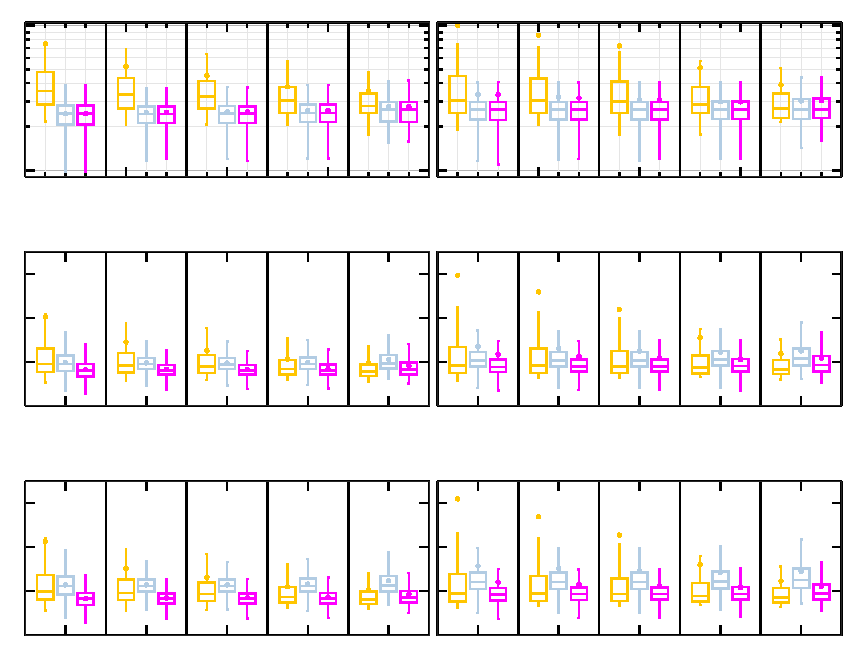
\includegraphics{./figures/parts/02/chapters/04/sections/05/boxplots_iterations}}%
    \gplfronttext
  \end{picture}%
\endgroup

  \end{figure}


  \placebottom
  \tiny [1] C. H. Walsh and S. Karaman, ``CDDT: Fast Approximate 2D Ray Casting for Accelerated Localization,", \textit{IEEE International Conference on Robotics and Automation}, 2018

\note{\footnotesize
Πάμε τώρα στο δεύτερο στόχο. Σε αυτή τη διαφάνεια βλέπουμε τους χρόνους
εκτέλεσης των τριών εκδόσεων του fsm2 για κάθε τιμή θορύβου μέτρησης και
διαφθοράς του χάρτη. Στην άνω σειρά βλέπουμε τα ευθεία αποτελέσματα από την
πειραματική διαδικασία και στην κάτω σειρά τους χρόνους εκτέλεσης που θα είχαν
οι μέθοδοι εάν ο χάρτης αναπαρίστατο ως εικόνα. Η διαφορά ανάμεσα στις δύο
αναπαραστάσεις είναι μεγάλη λόγω του χρόνου υπολογισμού εικονικών σαρώσεων που
είναι η πιό δαπανηρή πράξη, και που στην περίπτωση της αναπαράστασης μέσω
εικόνας μπορεί να γίνει στο ένα τρίτο του χρόνου σε σχέση με τον τρόπου που την
έχω υλοποιήσει εδώ. Τώρα: ο στόχος μας εδώ είναι κάθε μέθοδος να εκτελείται σε
μεγαλύτερη συχνότητα από τη συχνότητα παραγωγής εκτιμήσεων από το σύστημα που
εκτελεί το pose tracking, η οποία δεν έχει ακριβή ορισμό.  Στην πράξη αυτό που
θα θέλαμε είναι η συχνότητα εκτέλεσης να είναι τουλάχιστον 5 Hz.
Ο χαμηλότερος ρυθμός εκτέλεσης είναι της μεθόδου x1 όταν ο χάρτης είναι
διεφθαρμένος, κατά μέσο όρο στα 6.5 Hz, ενώ οι υπόλοιπες δύο μέθοδοι λειτουργούν
με τιμή περίπου στα 13 με 20 Hz.}

\end{frame}

\begin{frame}{\texttt{sm}\{$\cdot$,\texttt{2}\}: \texttt{I/O}}

  \noindent\makebox[\linewidth][c]{%
  \begin{minipage}{\linewidth}
    \begin{minipage}{0.3\linewidth}
      \begin{figure}
        
\definecolor{r}{RGB}{255 69 0}
\definecolor{b}{RGB}{51 102 153}


\tikzset{every picture/.style={line width=0.75pt}} %set default line width to 0.75pt

\begin{tikzpicture}[x=0.75pt,y=0.75pt,yscale=-1,xscale=1]
%uncomment if require: \path (0,300); %set diagram left start at 0, and has height of 300

%Straight Lines [id:da4529423263739871]
\draw   [color={rgb, 255:red, 255; green, 69; blue, 0 }  ] (61.5,52) -- (100.94,83.75) ;
\draw [shift={(102.5,85)}, rotate = 218.83] [color={rgb, 255:red, 255; green, 69; blue, 0 }  ][line width=0.75]    (10.93,-3.29) .. controls (6.95,-1.4) and (3.31,-0.3) .. (0,0) .. controls (3.31,0.3) and (6.95,1.4) .. (10.93,3.29)   ;
%Straight Lines [id:da6488911304441738]
\draw   [color={rgb, 255:red, 51; green, 102; blue, 153 }  ] (58.5,126) -- (100.71,104.89) ;
\draw [shift={(102.5,104)}, rotate = 153.43] [color={rgb, 255:red, 51; green, 102; blue, 153 }  ][line width=0.75]    (10.93,-3.29) .. controls (6.95,-1.4) and (3.31,-0.3) .. (0,0) .. controls (3.31,0.3) and (6.95,1.4) .. (10.93,3.29)   ;
%Straight Lines [id:da5938727374819561]
\draw  [color={rgb, 255:red, 255; green, 69; blue, 0 }  ]  (121.5,37) -- (122.45,75) ;
\draw [shift={(122.5,77)}, rotate = 270] [color={rgb, 255:red, 255; green, 69; blue, 0 }  ][line width=0.75]    (10.93,-3.29) .. controls (6.95,-1.4) and (3.31,-0.3) .. (0,0) .. controls (3.31,0.3) and (6.95,1.4) .. (10.93,3.29)   ;
%Straight Lines [id:da5792126615284177]
\draw    (135.5,94) -- (173.5,94) ;
\draw [shift={(175.5,94)}, rotate = 180] [color={rgb, 255:red, 0; green, 0; blue, 0 }  ][line width=0.75]    (10.93,-3.29) .. controls (6.95,-1.4) and (3.31,-0.3) .. (0,0) .. controls (3.31,0.3) and (6.95,1.4) .. (10.93,3.29)   ;

% Text Node
\draw    (107,82) -- (135,82) -- (135,107) -- (107,107) -- cycle  ;
\draw (121,94.5) node   [align=left] {\texttt{sm}};
% Text Node
\draw (35,32) node [anchor=north west][inner sep=0.75pt]   [align=left] {$\textcolor{r}{\mathcal{S}(\bm{p}_{k})}$};
% Text Node
\draw (34,127) node [anchor=north west][inner sep=0.75pt]   [align=left] {$\textcolor{b}{\mathcal{S}(\bm{p}_{k+1})}$};
% Text Node
\draw (113,17) node [anchor=north west][inner sep=0.75pt]   [align=left] {$\textcolor{r}{\bm{p}_{k}}$};
% Text Node
\draw (179,88) node [anchor=north west][inner sep=0.75pt]   [align=left] {$\textcolor{b}{\bm{p}_{k+1}}$};
\draw  [color={rgb, 255:red, 0; green, 255; blue, 0 }  ]  (195,94) circle [x radius= 16.26, y radius= 16.26]   ;


\end{tikzpicture}
        \caption{\scriptsize \texttt{sm}: ευθυγράμμιση πραγματικών σαρώσεων}
      \end{figure}
    \end{minipage}
    \hspace{1.2cm}
    \begin{minipage}{0.6\linewidth}
      \begin{figure}
        
\definecolor{r}{RGB}{255 69 0}
\definecolor{b}{RGB}{51 102 153}


\tikzset{every picture/.style={line width=0.75pt}} %set default line width to 0.75pt

\begin{tikzpicture}[x=0.75pt,y=0.75pt,yscale=-1,xscale=1]
%uncomment if require: \path (0,300); %set diagram left start at 0, and has height of 300

%Shape: Rectangle [id:dp6131376592433888]
\draw  [dash pattern={on 0.84pt off 2.51pt}] (322,78) -- (519.5,78) -- (519.5,157) -- (322,157) -- cycle ;
%Straight Lines [id:da45736430417167373]
\draw    (294.5,111) -- (325.5,111) ;
\draw [shift={(327.5,111)}, rotate = 180] [color={rgb, 255:red, 0; green, 0; blue, 0 }  ][line width=0.75]    (10.93,-3.29) .. controls (6.95,-1.4) and (3.31,-0.3) .. (0,0) .. controls (3.31,0.3) and (6.95,1.4) .. (10.93,3.29)   ;
%Straight Lines [id:da7019178260598848]
\draw   [color={rgb, 255:red, 51; green, 102; blue, 153 }  ] (293.5,172) -- (470.53,141.34) ;
\draw [shift={(472.5,141)}, rotate = 170.17] [color={rgb, 255:red, 51; green, 102; blue, 153 }  ][line width=0.75]    (10.93,-3.29) .. controls (6.95,-1.4) and (3.31,-0.3) .. (0,0) .. controls (3.31,0.3) and (6.95,1.4) .. (10.93,3.29)   ;
%Straight Lines [id:da9869567554869965]
\draw   [color={rgb, 255:red, 255; green, 69; blue, 0 }  ] (409.5,109) -- (470.56,123.51) ;
\draw [shift={(472.5,124)}, rotate = 194.04] [color={rgb, 255:red, 255; green, 69; blue, 0 }  ][line width=0.75]    (10.93,-3.29) .. controls (6.95,-1.4) and (3.31,-0.3) .. (0,0) .. controls (3.31,0.3) and (6.95,1.4) .. (10.93,3.29)   ;
%Straight Lines [id:da23755426444121874]
\draw    (397.5,37) -- (397.5,89) ;
\draw [shift={(397.5,91)}, rotate = 270] [color={rgb, 255:red, 0; green, 0; blue, 0 }  ][line width=0.75]    (10.93,-3.29) .. controls (6.95,-1.4) and (3.31,-0.3) .. (0,0) .. controls (3.31,0.3) and (6.95,1.4) .. (10.93,3.29)   ;
%Straight Lines [id:da07285087411586999]
\draw   [color={rgb, 255:red, 255; green, 69; blue, 0 }  ] (397.5,37) -- (487.97,112.72) ;
\draw [shift={(489.5,114)}, rotate = 219.93] [color={rgb, 255:red, 255; green, 69; blue, 0 }  ][line width=0.75]    (10.93,-3.29) .. controls (6.95,-1.4) and (3.31,-0.3) .. (0,0) .. controls (3.31,0.3) and (6.95,1.4) .. (10.93,3.29)   ;
%Straight Lines [id:da25729544560038]
\draw    (504.5,132) -- (543.5,132) ;
\draw [shift={(545.5,132)}, rotate = 180] [color={rgb, 255:red, 0; green, 0; blue, 0 }  ][line width=0.75]    (10.93,-3.29) .. controls (6.95,-1.4) and (3.31,-0.3) .. (0,0) .. controls (3.31,0.3) and (6.95,1.4) .. (10.93,3.29)   ;

% Text Node
\draw    (477,119) -- (505,119) -- (505,144) -- (477,144) -- cycle  ;
\draw (491,131.5) node   [align=left] {\texttt{sm}};
% Text Node
\draw (489,58) node [anchor=north west][inner sep=0.75pt]   [align=left] {\texttt{sm2}};
% Text Node
\draw (259,165) node [anchor=north west][inner sep=0.75pt]   [align=left] {$\textcolor{b}{\mathcal{S}(\bm{p})}$};
% Text Node
\draw (224,103) node [anchor=north west][inner sep=0.75pt]   [align=left] {Χάρτης $\bm{M}$};
% Text Node
\draw    (332.1,96) -- (409.1,96) -- (409.1,121) -- (332.1,121) -- cycle  ;
\draw (370.6,111) node   [align=left] {\texttt{scan\_map}};
% Text Node
\draw (393,16) node [anchor=north west][inner sep=0.75pt]   [align=left] {$\textcolor{r}{\hat{\bm{p}}}$};
% Text Node
\draw (422,95) node [anchor=north west][inner sep=0.75pt]   [align=left] {\footnotesize$\textcolor{r}{\mathcal{S}(\hat{\bm{p}})}$};
% Text Node
\draw (549,127) node [anchor=north west][inner sep=0.75pt]   [align=left] {$\textcolor{b}{\bm{p}}$};
\draw  [color={rgb, 255:red, 0; green, 255; blue, 0 }  ]  (556, 133) circle [x radius= 12.26, y radius= 12.26]   ;

\end{tikzpicture}
        \caption{\scriptsize \texttt{sm2}: ευθυγράμμιση πραγματικής σάρωσης με εικονική σάρωση χάρτη}
      \end{figure}
    \end{minipage}

  \end{minipage}
  }


\note{\footnotesize
Σε αυτό το γεγονός κρύβεται μία δεύτερη χρησιμότητα της ευθυγράμμισης σαρώσεων.
Εαν αντικαταστήσουμε τη μία από τις δύο μετρήσεις με μία εικονική σάρωση,
δηλαδή με μία σάρωση που προσομοιώνει την αρχή λειτουργίας του lidar στο χάρτη
αντί για το περιβάλλον, η οποία υπολογίζεται από την εκτίμηση της στάσης του
ρομπότ, τοτε μπορούμε να υπολογίσουμε το μετασχηματισμό ανάμεσα στην εκτίμηση
και την άγνωστη πραγματική στάση του ρομπότ, και αφού γνωρίζουμε την εκτίμηση,
μπορούμε να υπολογίσουμε την πραγματική του στάση.}


\end{frame}



\end{document}
